\documentclass[11pt,oneside]{book}
\usepackage{amsmath}
\usepackage{amssymb}
\usepackage{amsthm}
\usepackage{amsfonts}
\usepackage{multirow}
\usepackage{float}
\usepackage{diagbox}
\usepackage{xcolor}
\usepackage{caption}
\usepackage{graphicx}
\usepackage{subfigure}
\graphicspath{{img/}}
\usepackage{paralist}
\usepackage{tikz}
\let\itemize\compactitem
\let\enditemize\endcompactitem
\let\enumerate\compactenum
\let\endenumerate\endcompactenum
\let\description\compactdesc
\let\enddescription\endcompactdesc
\setlength{\parindent}{0pt}
\title{Answer book of Hungerford Algebra}
\author{}
\date{}
\newtheorem{theorem}{Theorem}[section]
\newtheorem*{lemma}{Lemma}
\newtheorem{definition}{Definition}[section]
\theoremstyle{definition}
\newtheorem{ex}{Exercise}[section]
\newtheorem*{answer}{Answer}
\newcommand\thmref[1]{\textbf{Theorem \ref{#1}}}
\newcommand\figref[1]{\textbf{Figure \ref{#1}}}
\begin{document}
\newtheorem*{tips}{\emph{TIPS}}
\chapter{Groups}
\section{Logical Symbols}
The logical symbols are a kind of symbols using for theoretical statements.
    \begin{table}[H]
        \centering
        \caption{Frequently-used Logical Symbols}
        \begin{tabular}{|c|c|}\hline
            Symbols&Meanings\\\hline
            $L\Longrightarrow P$& Proposition $L$ is contained in proposition $P$\\
            $L \Longleftrightarrow P $&Proposition $L$ is equivalent to proposition $P$\\
            $\lnot P$&Not $P$\\
            $L\wedge P$&Proposition $L$ and proposition $P$\\
            $L \vee P$&Proposition $L$ or proposition $P$\\
            \hline
        \end{tabular}
    \end{table}
e.g.\[((A\Longrightarrow B)\wedge(\lnot B)\Longrightarrow (\lnot A) )\]


stands for `` if $A$ is contained in  $B$,and $B$ is not true,then $A$ is not true''.

We also call $ A \Longleftrightarrow B$ ``$A$ is the necessary and suffiecent condition of $B$''.

The typical math proposition is like ``$A\Longrightarrow B$''.In order to prove this proposition ,we can use the  implication relationship \[A\Longrightarrow C_1\Longrightarrow \cdots \Longrightarrow C_n\Longrightarrow B\]The every implication relationship in this chain is general truth or proved proposition.

\begin{table}[H]
    \centering
    \caption{Truth Table}
    \begin{tabular}{|c|c|c|c|}
        \hline
        \multirow{2}{*}{$\lnot A$}                       & $A$                    & 0         & 1             \\ \cline{2-4} 
                                                 & $\lnot A$            & 1            & 0             \\ \hline
        \multirow{3}{*}{$A \vee B$}                       &       \diagbox{$A$}{$B$}     &    0        &       1        \\ \cline{2-4} 
                                                 &          0       &   0         &        1        \\ \cline{2-4} 
                                                 &       1         &  1        &        1       \\ \hline
        \multirow{3}{*}{$A \wedge B$}                       &        \diagbox{$A$}{$B$}    &           0&        1          \\ \cline{2-4} 
                                                 &     0         &     0          &      0          \\ \cline{2-4} 
                                                 &        1        &                0       &    1       \\ \hline
        \multirow{3}{*}{$A\Longrightarrow B$}                      &  \diagbox{$A$}{$B$} & 0  &  1 \\ \cline{2-4} 
                                                & 0  &  1 &  1 \\ \cline{2-4} 
                                                & 1  &  0 & 1  \\ \hline
        \end{tabular}
    \end{table}
\begin{question}$\lnot (A\wedge B )\Leftrightarrow (\lnot A \vee \lnot B)$.
\end{question}
\begin{proof}
    (Use the truth table)

    If $A$ is ture, $B$ is ture, $A\wedge B$ is ture. $\lnot (A\wedge B)$ is false.$\lnot A $ is false,$\lnot B$ is false, $(\lnot A \vee \lnot B)$ is false.

    If $A$ is ture, $B$ is false, $A\wedge B$ is false. $\lnot (A\wedge B)$ is true.$\lnot A $ is false,$\lnot B$ is true, $(\lnot A \vee \lnot B)$ is ture.

    If $A$ is flase, $B$ is true, $A\wedge B$ is false. $\lnot (A\wedge B)$ is true.$\lnot A $ is true,$\lnot B$ is false, $(\lnot A \vee \lnot B)$ is ture.

    If $A$ is false, $B$ is false, $A\wedge B$ is false. $\lnot (A\wedge B)$ is true.$\lnot A $ is true,$\lnot B$ is true, $(\lnot A \vee \lnot B)$ is ture.

    So
    \[\lnot (A\wedge B )\Leftrightarrow (\lnot A \vee \lnot B)\]
\end{proof}    

\begin{question}
    $(A \Rightarrow B)\Leftrightarrow\lnot A \vee B$.
\end{question}
\begin{proof}
    Firstly, we confirm the truth of \[(A \Rightarrow B)\Rightarrow\lnot A \vee B\]

    If $(A \Rightarrow B)$ is false, then $\lnot A \vee B$ is true.

    If $(A \Rightarrow B)$ is ture ,then we have two posibilities. The first is $A$ is ture, $B$ is true, so $\lnot A \vee B$ is true. The second is $A$ is false,then $B$ can be true or false, but $\lnot A \vee B$ will be true.

    Hence, $(A \Rightarrow B)\Rightarrow\lnot A \vee B$.

    Secondly, we prove \[(A \Rightarrow B)\Leftarrow\lnot A \vee B\]

    If $\lnot A \vee B$ is false, then $(A \Rightarrow B)$ is true.

    If $\lnot A \vee B$ is true, we have
    \begin{enumerate}
        \item $\lnot A$ is true, $B$ is false, then, $A$ is false, $(A \Rightarrow B)$ is true.
        \item $\lnot A$ is false, $B$ is true, then, $A$ is true, $(A \Rightarrow B)$ is true.
        \item $\lnot A$ is true, $B$ is true, then, $A$ is false, $(A \Rightarrow B)$ is true.
    \end{enumerate}

    So $(A \Rightarrow B)\Leftarrow\lnot A \vee B$.
\end{proof}



\section{Homomorphisms and subgroups}
\begin{ex}
    If $f: G \to H$ is a homomorphism of groups, then $f(e_G) = e_H$ and $f(a^{-1}) = f(a)^{-1}$ for all $a \in G$. Show by example that the first conclusion may be false if $G$, $H$ are monoids that are not groups.
\end{ex}

$$ $$

\begin{ex}
    A group $G$ is abelian if and only if the map $G\to G$ given by $x\to x^{-1}$ is automorphism.
\end{ex}

$$ $$

\begin{ex}
    Let $Q_8$ be the group(under ordinary matrix multiplication) generated by complex matrices $A = \begin{pmatrix}
        0 & 1 \\
        -1 & 0
    \end{pmatrix}$ and $B = \begin{pmatrix}
        0 & i\\
        i & 0
    \end{pmatrix}$, where $i^{2}=-1$. Show that $Q_8$ is a nonabelian group of order 8. $Q_8$ is called the quaternion group.
\end{ex}

$$ $$

\begin{ex}
    Let $H$ be the group(under ordinary matrix multiplication) of real matrices generated by $C = \begin{pmatrix}
        0 & 1\\
        -1 & 0
    \end{pmatrix}$ and $D = \begin{pmatrix}
        0 & 1\\
        1 & 0
    \end{pmatrix}$. Show that $H$ is a nonabelian group of order 8 which is not isomorphic to the quaternion group, but is isomorphic to the group $D_4^*$.
\end{ex}

$$ $$

\begin{ex}
    Let $S$ be a nonempty subset of a group $G$ and define a relation on $G$ by $a ~ b$ if and only if $ab^{-1}\in S$. Show that $~$ is an equivalence relation if and only if $S$ is a subgroup of $G$.
\end{ex}

$$ $$

\begin{ex}
    A nonempty finte subset of a group is s subgroup if and only if it is closed under the product in $G$.
\end{ex}

$$ $$

\begin{ex}
    If $n$ is a fixed integer, then $\{kn | n\in \mathbf{Z}\}\subset\mathbf{Z}$ is an additive subgroup of $\mathbf{Z}$, which is isomorphic to $\mathbf{Z}$. 
\end{ex}

$$ $$

\begin{ex}
    The set $\{\sigma\in S_n | \sigma(n) = n\}$ is a subgroup of $S_n$ which is isomorphic to $S_{n-1}$.
\end{ex}

$$ $$

\begin{ex}
    Let $f: G\to H$ be a homomorphism of groups, $A$ a subgroup of $G$, and $B$ a subgroup of $H$.
    \begin{enumerate}
        \item $\mathrm{Ker} f$ and $f^{-1}(B)$ are subgroups of $G$.
        \item $f(A)$ is a subgroup of $H$.
    \end{enumerate}
\end{ex}

$$ $$

\begin{ex}
    List all subgroups of $Z_2\oplus Z_2$. Is $Z_2\oplus Z_2$ isomorphic to $Z_4$?
\end{ex}

$$ $$

\begin{ex}
    If $G$ is a subgroup, then $C = \{a\in G| ax = xa \text{ for all } x\in G\}$ is a abelian subgroup of $G$. $C$ is called the center of $G$.
\end{ex}

$$ $$

\begin{ex}
    The group $D_4^*$ is not cyclic, but can be generated by two elements. The same is true of $S_n$(nontrivial). What is the minimal number of generators of the additive group $\mathbf{Z}\oplus\mathbf{Z}$?
\end{ex}

$$ $$

\begin{ex}
    If $G = \left\langle a \right\rangle $ is a cyclic group and $H$ is any group, then every homomorphism $f:G\to H$ is completely determined by the element $f(a)\in H$.
\end{ex}

$$ $$

\begin{ex}
    The following cyclic subgroups are all isomorphic: the multiplication group $\left\langle i \right\rangle$ in $\mathbf{C}$, the additive group $\mathbf{Z_4}$ and the subgroup $\left\langle \begin{pmatrix}
        1 & 2 & 3 & 4\\
        2 & 3 & 4 & 1
    \end{pmatrix}\right\rangle$ of $S_4$.
\end{ex}

$$ $$

\begin{ex}
    Let $G$ be a group and $\mathrm{Aut} G$ is the set of all automorphisms of $G$.
    \begin{enumerate}
        \item $\mathrm{Aut} G$ is a group with composition of functions as binary operation.
        \item $\mathrm{Aut} \mathbf{Z}\cong Z_2$ and $\mathrm{Aut} Z_6 \cong Z_2$; $\mathrm{Aut} Z_8\cong Z_2\oplus Z_2$; $\mathrm{Aut} Z_p\cong Z_{p-1}$ ($p$ prime).
        \item What is $\mathrm{Aut Z_n}$ for arbitrary $n\in \mathbf{N^*}$?
    \end{enumerate}
\end{ex}

$$ $$

\begin{ex}
    For each prime $p$ the additive subgroup $Z(p^\infty)$ of $\mathbf{Q}/\mathbf{Z}$ is generated by the set $\{\bar{1/p^n}|n\in \mathbf{N^*}\}$.
\end{ex}

$$ $$

\begin{ex}
    Let $G$ be an abelian group and let $H, K$ be subgroups of $G$. Show that the join $H\vee K$ is the set $\{ab|a\in H, b\in K\}$. Extend this result to any finite number of subgroups of $G$.
\end{ex}

$$ $$

\begin{ex}
    \begin{enumerate}
        \item Let $G$ be a group and $\{H_i| i\in I\}$ a family of subgroups. State and prove a condition that will imply that $\bigcup\limits_{i\in I}H_i$ is a subgroup, that is $\bigcup\limits_{i\in I}H_i = \left\langle\bigcup\limits_{i\in I}H_i\right\rangle$.
        \item Given an example of a group $G$ and a family of subgroups $\{H_i|i \in I\}$ such that $\bigcup\limits_{i\in I}H_i \neq \left\langle\bigcup\limits_{i\in I}H_i\right\rangle$.
    \end{enumerate}
\end{ex}

$$ $$

\begin{ex}
    \begin{enumerate}
        \item The set of all subgroups of a group $G$, partially ordered by set theoretic inclusion, forms a complete lattice in which the g.l.b of $\{H_i|i\in I\}$ is $\bigcap\limits_{i\in I}H_i$ and the l.u.b is $\left\langle\bigcap\limits_{i\in I}H_i\right\rangle$.
        \item Exhibit the lattice of subgroups of the groups $S_3, D_4^*, Z_6, Z_{27}$ and $Z_{36}$.
    \end{enumerate}
\end{ex}
\section{Cyclic groups}
\begin{ex}
    Let $a,b$ be elements of group $G$. Show that $\left| a \right| =\left| a^{-1} \right| $; $\left| ab \right| =\left| ba \right| $, and $\left| a \right| =\left| cac^{-1} \right| $ for all $c\in G$.
\end{ex}

\begin{answer}
    We only consider that $\left| a \right| , \left| b \right| , \left| c \right| $ are finite. Assume $a^{k}=e$, $(ab)^{m}=e$, $(ac^{-1})^{n}=e$, $kmn\neq 0$. $a^{k}\cdot(a^{-1})^{k}=e$, so $k$ sialso the order of $a^{-1}$, $\left| a^{-1} \right| =k$. $(ab)^{m}=e=a(ba)^{m-1}b\Rightarrow (ba)^{m-1}=a^{-1}b^{-1}$, $(ba)^{m}=a^{-1}b^{-1}ba=e$. $m$ is the order of $ba$. $(cac^{-1})^{r}=cac^{-1}cac^{-1}\cdots cac^{-1}=ca^{n}c^{-1}=e$, so $a^{n}=e$, whence $n=k$.
\end{answer}

$$ $$

\begin{ex}
    Let $G$ be an abelian group containing elements $a$ and $b$ of orders $m$ and $n$ respectively. Show that $G$ contains an element whose order is the least commom multiple of $m$ and $n$.
\end{ex}

\begin{answer}
    If $(m,n)=1$, we know that $\forall a^{i}, i=1,2,\dots, m$, $b^{j}, j=1, 2, \dots, n$, $a^{i}b^{j}\neq e$, since if $a^{i}=b^{j}$, $\left| a^{i} \right| =n=\left| b^{-j} \right| =\left| b^{j} \right| =m$. $G$ is abelian, so $(ab)^{k}=a^{k}b^{k}\Rightarrow \left| ab \right|=mn=\left[ m,n\right]$.

    If $m|n$ or $n|m$, then $a$ or $b$ is the element we want. We consider $m|\!\!/n$ and $n|\!\!/m$. Factorise $n=p_{1}^{t_{1}}p_{2}^{t_{2}}\cdots p_{l}^{t_{l}}$, $m=p_{1}^{s_{1}}p_{2}^{s_{2}}\cdots p_{l}^{s_{l}}$, where $p_{1},\cdots,p_{l}$ are primes and $t_{1},\cdots,t_{l}, s_{1},\cdots, s_{l}\geq 0$. We can choose a new arrangement of $p_{1},\cdots,p_{l}$ and make $t_{1}\geq s_{1}$, $t_{2}\geq s_{2}$,\dots, $t_{i}\geq s_{i}$, $t_{i+1}<s_{i+1}$,\dots, $t_{l}<s_{l}$.\[(m,n)=p_{1}^{s_{1}}\cdots p_{i}^{s_{i}}p_{i+1}^{t_{i+1}}\cdots p_{l}^{t_{l}}, \left[m,n\right]=p_{1}^{t_{1}}\cdots p_{i}^{t_{i}}p_{i+1}^{s_{i+1}}\cdots p_{l}^{s_{l}}\] Take $x=a^{{p_{i+1}^{s_{i+1}}}\cdots p_{l}^{s_{l}}}$, $y=b^{{p_{1}^{t_{1}}}\cdots p_{i}^{t_{i}}}$, then $\left| x \right| ={p_{1}^{t_{1}}}\cdots p_{i}^{t_{i}}$, $\left| y \right| =p_{i+1}^{s_{i+1}}\cdots p_{l}^{s_{l}}$. Thus $(x,y)=1$, the order of $xy$ is $\left| x \right| \cdot\left| y \right| =p_{1}^{t_{1}}\cdots p_{i}^{t_{i}}p_{i+1}^{s_{i+1}}\cdots p_{l}^{s_{l}}=\left[m,n\right]$.
\end{answer}

$$ $$

\begin{ex}
    Let $G$ be an abelian group of order $pq$, with $(p,q)=1$. Assume there exist $a,b\in G$ such that $\left| a \right| =p, \left| b \right| =q$ and show that $G$ is cyclic.
\end{ex}

\begin{answer}
    From \textbf{Exercise 1.3.2} we know $a^{i}b^{j}\neq e$ for $i<p$, $j<q$. $\left| G \right| =pq$ for all $a^{i}b^{j}$ and $a^{m}b^{n}$ with $i\neq m$, $b\neq n$, $a^{i}b^{j}\neq a^{m}b^{n}$. So $G$ can be generated by $ab$. $G$ is cyclic.
\end{answer}

$$ $$

\begin{ex}
    If $f:G\to H$ is a homomorphism, $a\in G$, and $f(a)$ has finte order in $H$, then $\left| a \right| $ is infinite or $\left| f(a) \right| $ divides $\left| a \right| $.
\end{ex}

\begin{answer}
    Assume $\left| f(a) \right| =n$, $\left| a \right| =m$, and $n|\!\!/m$. Trivially, $m\geq n$. Assume $\gcd(m,n)=k\leq n$. $a^{m}=e\Rightarrow f(a)^{m}=e'=f(a)^{n}$. By Bezout theorem $\exists x,y\in \mathbf{Z}$ s.t. $f(a)^{mx+ny}=f(a)^{k}=e'$, $k\leq n$, that's contradictory!
\end{answer}

$$ $$

\begin{ex}
    Let $G$ be the multiplicative group of all nonsingular $2\times 2$ matrices with rational entries. Show that $a=\begin{pmatrix}
        0 & -1\\1 & 0
    \end{pmatrix}$has order 4 and $b=\begin{pmatrix}
        0& 1\\-1&-1
    \end{pmatrix}$has order 3, but $ab$ has infinite order. Conversely, show that the additive group $Z_{2}\oplus \mathbf{Z}$ contains nonzero elements $a,b$ of infinite order such that $a+b$ has finite order. 
\end{ex}

\begin{answer}
    The verification of $\left| a \right| =4$ and $\left| b \right| =3$ is trivial. $ab=\begin{pmatrix}
        1 & 1\\ 0& 1
    \end{pmatrix}$ $\det(ab=\lambda I)=0\Rightarrow \lambda_{1}=\lambda_{2}=1$. $ab$ is not diagnizable. By induction, we have $(ab)^{n}=\begin{pmatrix}
        1 & 2^{n-1}\\ 0& 1
    \end{pmatrix}$ which means $(ab)$ has infinite order.

    For $a=(\bar{0},1), b=(\bar{0},-1)\in Z_{2}\oplus\mathbf{Z}$, $a,b$ have infinite order, but $a+b=(\bar{0},0)$ has finite order 1.
\end{answer}

$$ $$

\begin{ex}
    If $G$ is a cyclic group of order $n$ and $k| n$, then $G$ has exactly one subgroup of order $k$.
\end{ex}

\begin{answer}
    Assume $a^{n}=e$, $mk=n$, we verify that $\left\langle a^{m}\right\rangle$ is a subgroup of order $k$. $\forall x,y\in \mathbf{Z}_{+}$, $a^{xm}\cdot a^{-ym}=a^{(x-y)m}\in \left\langle a^{m}\right\rangle$, so $\left\langle a^{m}\right\rangle$ is a subgroup. $a^{km}=e$, $a^{sm}\neq e$ for $s<k$, so $\left| \left\langle a^{m}\right\rangle \right| =k$.
\end{answer}

$$ $$

\begin{ex}
    Let $p$ be prime and $H$ a subgroup of $Z(p^{\infty})$.
    \begin{enumerate}[(a)]
        \item Every element of $Z(p^{\infty})$ has finite order $p^{n}$ for some $n\geq 0$.
        \item If at least one element of $H$ has order $p^{k}$ and no element of $H$ has order greater than $p^{k}$, then $H$ is the cyclic subgroup generated by $\bar{1/p^{k}}$, whence $H\cong Z_{p^{k}}$.
        \item If there is no upper bound on the orders of elements of $H$, then $H=Z(p^{\infty})$.
        \item The only proper subgroups of $Z(p^{\infty})$ are the finite cyclic groups $C_{n}=\left\langle\bar{1/p^{n}}\right\rangle\,(n=1,2,\dots)$. Futhermore, $\left\langle0\right\rangle=C_{0}<C_{1}<C_{2}<C_{3}<\cdots$.
        \item Let $x_{1},x_{2},\dots$ be elements of an abelian group $G$ such that $\left| x_{1} \right| =p, px_{2}=x_{1},px_{3}=x_{2},\dots,px_{n+1}=x_{n},\dots$. The subgroup generated by the $x_{i}(i\geq 1)$ is isomorphic to $Z(p^{\infty})$. 
    \end{enumerate}
\end{ex}

\begin{answer}
    \begin{enumerate}[(a)]
        \item $\forall  x\in Z(p^{\infty})$, $x=\frac{a}{p^{n}}$ where $a<p^{n}$, $p|\!\!/a$. $p$ is a prime, so $\gcd(p,a)=1$. $m\cdot a|p^{n}\Rightarrow m=p^{n}$. Thus $m\cdot \frac{a}{p^{n}}=e$, $p^{n}$ is the smallest number satisfies it. $\frac{a}{p^{n}}$ has order $p^{n}$.
        \item For all $x\in Z(p^{\infty})$, if $x$ has order smaller than $p^{k}$, $x$ must have the form $x=\frac{a}{p^{i}}(i\leq k)$, $(p,a)=1$, so $x\in\left\langle\frac{1}{p^{k}}\right\rangle$. If not, assume $x=\frac{a}{p^{i}}(i>k)$, then $p^{k}\cdot x=\frac{a}{p^{i-k}}\neq 1$.
        \item Assume not, $H< Z(p^{\infty})$, $H\neq Z(p^{\infty})$. There exist $y\in H$ s.t. $y$ has order $p^{m}, m\geq n$. $y=\frac{b}{p^{m}}$, $(p,b)=1$, so there exists $b^{-1}\in\{1,2,\dots,p-1\}$, $bb^{-1}\equiv 1\mod p^{m}$. But $ab^{-1}p^{m-n}y=\frac{a}{p^{n}}=x\in H$, that's contradictory! Conversely, $H=Z(p^{\infty})$.
        \item From (b), we know that if there's least upper bound $p^{n}$ for elements in a subgroup $S$, then $S=C_{n}$.\[\left\langle0\right\rangle=C_{0}<C_{1}<C_{2}<C_{3}<\cdots<Z(p^{\infty})\] is easy to verify.
        \item We can verify that $f:x_{i}\mapsto \bar{\frac{1}{p^{i}}}$ is a well defined isomorphism. $f(e)=f(px_{1})=1$, $f(px_{i+1})=f(x_{i})=\frac{1}{p^{i}}=p\cdot \frac{1}{p^{i+1}}$. $f$ is obviously a bijection, so $H\cong Z(p^{\infty})$.
    \end{enumerate}
\end{answer}

$$ $$

\begin{ex}
    A group that has only a finite number of subgroups must be finite.
\end{ex}

\begin{answer}
    Suppose not. If the order of all subgroups are finite, $G$ must be finite. So there exists a infinite subgroup $H<G$. $\forall  a\in G$, if $\forall n\in \mathbf{N}$, $a^{n}\neq e$. then we can construct infinte subgroups $\left\langle a\right\rangle$, $\left\langle a^{2}\right\rangle$, $\left\langle a^{3}\right\rangle$\dots. If $\forall a\in G$, $\exists n\in \mathbf{N}$, $a^{n}=e$, so $\left\langle a\right\rangle$ is a proper subgroup of $G$, we can take $b\in G\backepsilon\left\langle a\right\rangle$ to construct another subgroup. By induction, there are infinte subgroups in $G$. That's contradictory, so $G$ must be finite.
\end{answer}

$$ $$

\begin{ex}
    If $G$ is an abelian group, then the set $T$ of all elements of $G$ with finite order is a subgroup of $G$.
\end{ex}

\begin{answer}
    We can easily verify that $\forall a,b\in S$, $\left| a \right| =m$, $\left| b \right| =n$ and $\left| ab^{-1} \right| \leq mn$ is finite. $T$ is a subgroup of $G$.
\end{answer}

$$ $$

\begin{ex}
    An infinite group is cyclic if and only if it is isomorphic to each of its proper subgroups.
\end{ex}

\begin{answer}
    If $G$ is cyclic, $G\cong \mathbf{Z}$, $S<G$. For any subgroup of $\mathbf{Z}$, it has the form $\{na\}, a\in \mathbf{Z}$. We can construct a isomorphism $f:n\mapsto na$, so $S\cong \{na\}\Rightarrow G\cong S$.

    If $\forall S<G$, $G\cong S$ and $\left| G \right| =\left| S \right| $ is finite. We prove there exists $S<G$ s.t. $\left| S \right| =\aleph_{0}$. Take $a\in G$ and $S=\{na|n\in \mathbf{Z}\}$, $S$ is a subgroup. If there exists $ma=0$, $S$ must be finite, contradictory! Thus, $S\cong \mathbf{Z}\cong G$. $G$ is a infinite cyclic group.
\end{answer}
\section{Cosets and counting}
\begin{ex}
    Let $G$ be a group and $\{H_{i}|i\in I\}$ a family of subgroups. Then for any $a\in G$, $(\bigcap\limits_{i}H_{i})a=\bigcap\limits_{i}H_{i}a$.
\end{ex}

$$ $$

\begin{ex}
    \begin{enumerate}[(a)]
        \item Let $H$ be the cyclic subgroup (of order 2) of $S_{3}$ generated by $\begin{pmatrix}
            1 & 2 &3\\2& 1&3
        \end{pmatrix}$. Then no left cosets of $H$ (except $H$ itself) is also a right coset. There exists $a\in S_{3}$ such that $aH\cap Ha=\{a\}$.
        \item If $K$ is the cyclic subgroup (of order 3) of $S_{3}$ generated by $\begin{pmatrix}
            1 & 2&3\\2& 3 &1
        \end{pmatrix}$, then every left coset of $K$ is also a right coset of $K$.
    \end{enumerate}
\end{ex}

$$ $$

\begin{ex}
    The following conditions on a finite group $G$ are equivalent.
    \begin{enumerate}[(i)]
        \item $\left| G \right| $ is prime.
        \item $G\neq \left\langle e\right\rangle$ and $G$ has no proper subgroups.
        \item $G\cong Z_{p}$ for some prime $p$.
    \end{enumerate}
\end{ex}

$$ $$

\begin{ex}
    Let $a$ be an integer and $p$ be a prime such that $p\nmid a$. Then $a^{p-1}\equiv 1\mod p$.
\end{ex}

$$ $$

\begin{ex}
    Prove that there are only two distinct groups of order 4 (up to isomorphism), namely $Z_{4}$ and $Z_{2}\oplus Z_{2}$.
\end{ex}

$$ $$

\begin{ex}
    Let $H,K$ be subgroups of a group $G$. Then $HK$ is a subgroup of $G$ if and only if $HK=KH$.
\end{ex}

$$ $$

\begin{ex}
    Let $G$ be a group of order $p^{k}m$, with $p$ prime and $(p,m)=1$. Let $H$ be a subgroup of order $p^{k}$ and $K$ a subgroup of order $p^{d}$, with $0<d\leq k$ and $K\not\subset H$. Show that $HK$ is not a subgroup of $G$.
\end{ex}

$$ $$

\begin{ex}
    If $H$ and $K$ are subgroups of finite index of a group $G$ such that $\left[G:H\right]$ and $\left[G:K\right]$ are relatively prime, then $G=HK$.
\end{ex}

$$ $$

\begin{ex}
    If $H,K$ and $N$ are subgroups of a group $G$ such that $H<N$, then $HK\cap N=H(K\cap N)$. 
\end{ex}

$$ $$

\begin{ex}
    Let $H,K,N$ be subgroups of a group $G$ such that $H<K$, $H\cap N=K\cap N$, and $HN=KN$. Show that $H=K$.
\end{ex}

$$ $$

\begin{ex}
    Let $G$ be a group of order $2n$; then $G$ contains an element of order 2. If $n$ is odd and $G$ abelian, there is only one element of order 2.
\end{ex}

$$ $$

\begin{ex}
    If $H$ and $K$ are subgroups of a group $G$, then $\left[H\vee K:H\right]\\\geq \left[K:H\cap K\right]$.
\end{ex}

$$ $$

\begin{ex}
    If $p>q$ are primes, a group of order $pq$ has at most one subgroup of order $p$.
\end{ex}

$$ $$

\begin{ex}
    Let $G$ be a group and $a,b\in G$ such that (i) $\left| a \right| =4=\left| b \right| $; (ii) $a^{2}=b^{2}$; (iii) $ba=a^{3}b=a^{-1}b$; (iv) $a\neq b$; (v) $G=\left\langle a,b\right\rangle$. Show that $\left| G \right| =8$ and $G\cong Q_{8}$.
\end{ex}
\section{Normality, quotient groups, and homomorphisms}
\begin{ex}
    If $N$ is a subgroup of index 2 in a group $G$, then $N$ is normal in $G$.
\end{ex}

\begin{answer}
    $\forall a\in G\backslash N$, $G=N\cup Na=N\cup aN$ and $N\cap Na=\varnothing$, $N\cap aN=\varnothing$. So $\forall x\in Na$, $x\in G\backslash N\Rightarrow x\in aN$, $Na\subset aN$. Similarly, $aN\subset Na$, whence $Na=aN$, $N\lhd G$.
\end{answer}

$$ $$

\begin{ex}
    If $\{N_{i}|i\in I\}$ is a family of normal subgroups of a group $G$, then $\bigcap\limits_{i\in I}N_{i}$ is a normal subgroup of $G$.
\end{ex}

\begin{answer}
    $\bigcap\limits_{i\in I}N_{i}$ is a subgroup of $G$. $N_{i} (i\in I)$ are normal subgroups of $G$, so $\forall a\in G$, $aN_{i}a^{-1}=\{an_{i}a^{-1}|n_{i}\in N_{i}\}=N_{i}$. $\forall x=ana^{-1}\in a(\bigcap\limits_{i\in I}N_{i})a^{-1}$, $n\in N_{i}\Rightarrow x\in a(\bigcap\limits_{i\in I}N_{i})a^{-1}\subset \bigcap\limits_{i\in I}aN_{i}a^{-1}=\bigcap\limits_{i\in I}N_{i}$. $\bigcap\limits_{i\in I}N_{i}$ are normal subgroup of $G$.
\end{answer}

$$ $$

\begin{ex}
    Let $N$ be a subgroup of a group $G$. $N$ is normal in $G$ if and only if (right) congruence modulo $N$ is a congruence relation on $G$.
\end{ex}

\begin{answer}
    If $N\lhd G$. $\forall a,b\in G$, $ab^{-1}\in N\Leftrightarrow a^{-1}b\in N$. If $a_{1}\equiv b_{1}\mod N$, $a_{2}\equiv b_{2}\mod N$, then $a_{2}b_{2}^{-1}\in N$, $a_{1}N=Na_{1}=Nb_{1}\Rightarrow a_{1}Nb_{1}^{-1}=N$. So $a_{1}a_{2}b_{1}^{-1}b_{2}^{-1}=(a_{1}a_{2})(b_{1}b_{2})^{-1}\in N$. Similarly, $(a_{1}a_{2})^{-1}(b_{1}b_{2})\in N$. Congruence modulo $N$ is a congruence relation.

    If congruence modulo $N$ is a congruence relation. $\forall a_{1}\equiv b_{1}\mod N$, $a_{2}\equiv b_{2}\mod N$, we will have $a_{1}a_{2}\equiv b_{1}b_{2}\mod N$. Take $n\in N$ and fix $a_{2}\in G$, define $b_{2}=n^{-1}a_{2}$. Then $\forall n\in N$, $n$ can be expressed as $a_{2}b_{2}^{-1}$, $a_{2}\equiv b_{2}\mod N$. $\forall a_{1}\in G$ and $\forall b_{1}\equiv a_{1}\mod N$, $a_{1}nb_{1}^{-1}=a_{1}a_{2}b_{2}^{-1}b_{1}^{-1}\in N$. Take $b_{1}=a_{1}$ and $n$ varies in $N$, $a_{1}na_{1}^{-1}\in N\Rightarrow a_{1}Na_{1}^{-1}\subset N$. Thus $N\lhd G$.
\end{answer}

$$ $$

\begin{ex}
    Let $\sim$ be an equivalence relation on a group $G$ and let $N=\{a\in G |a\sim e\}$. Then $\sim$ is a congruence relation on $G$ if and only if $N$ is a normal subgroup of $G$ and $\sim$ is congruence modulo $N$.
\end{ex}

\begin{answer}
    If $G\lhd N$ and $\sim$ is congruence modulo $N$. $\forall a\in G$, $aNa^{-1}\subset N$. $\forall a_{1}, b_{1}, a_{2}, b_{2}\in G$, $a_{1}b_{1}^{-1}\in N$, $a_{2}b_{2}^{-1}\in N$. $a_{1}a_{2}(b_{1}b_{2})^{-1}=a_{1}a_{2}b_{2}^{-1}b_{1}^{-1}$, denote $n=a_{2}b_{2}^{-1}\in N$, $a_{1}a_{2}b_{2}^{-1}b_{1}^{-1}=a_{1}nb_{1}^{-1}\in a_{1}Nb_{1}^{-1}$. $\forall n\in N$, there exists $n'=b_{1}^{-1}a_{1}, n'\in N$ s.t. $a_{1}n=b_{1}n'$. So $a_{1}nb_{1}^{-1}=b_{1}n'b_{1}^{-1}\in b_{1}Nb_{1}^{-1}\subset N$. That means $(a_{1}a_{2})(b_{1}b_{2})^{-1}\in N$, $a\sim b$ is a congruence relation.

    If $a\sim b$ is a congruence relation. We first prove $N$ is a subgroup of $G$. $\forall a\in N$, $a\sim e$, $a^{-1}\sim a^{-1}\Rightarrow e\sim a^{-1}$, so $a^{-1}\sim e$, $a^{-1}\in N$. $\forall a,b \in N$, $b^{-1}\sim e$, $a\sim e\Rightarrow ab^{-1}\in e$, thus $N<G$.

    $\forall x\in G$, $xN=\{xa|a\sim e\}=\{xa|xa\sim xe\}=\{ax|ax\sim e\}=Nx$, so $N$ is normal in $G$. $x\sim y\Leftrightarrow y\in xN$. $\sim$ is congruence modulo $N$.
\end{answer}

$$ $$

\begin{ex}
    Let $N<S_{4}$ consist of all those permutations $\sigma$ such that $\sigma(4)=4$. Is $N$ normal in $S_{4}$?
\end{ex}

\begin{answer}
    $N=\{(1),(12),(13),(23),(123),(132)\}$. Take $a=(14)\in G$, $a^{-1}=(14)$, $a^{-1}(12)a=(24)\notin N$. So $N$ is not normal in $S_{4}$.
\end{answer}

$$ $$

\begin{ex}
    Let $H<G$; then the set $aHa^{-1}$ is a subgroup for each $a\in G$, and $H\cong aHa^{-1}$. 
\end{ex}

\begin{answer}
    $H<G$, $aHa^{-1}=\{aha^{-1}|h\in H\}$. $\forall x,y\in aHa^{-1}$, $x=ah_{1}a^{-1}$, $y=ah_{2}a^{-1}$. $y^{-1}=ah_{2}^{-1}a^{-1}$, $xy=ah_{1}h_{2}^{-1}a^{-1}\in aHa^{-1}$, so $aHa^{-1}< G$.

     Take $f: H\to aHa^{-1}$ as $f(h)=aha^{-1}$. If $f(h_{1})=f(h_{2})=ah_{1}a^{-1}=ah_{2}a^{-1}$, then $h_{1}=h_{2}$, so $f$ is an injection. $f$ is a surjection because $\forall x\in aHa^{-1}$, $f(a^{-1}xa)=x$, $a^{-1}xa\in H$. In conclusion, $H\cong aHa^{-1}$.
\end{answer}

$$ $$

\begin{ex}
    Let $G$ be a finite group and $H$ a subgroup of $G$ of order $n$. If $H$ is the only subgroup of $G$ of order $n$, then $H$ is normal in $G$.
\end{ex}

\begin{answer}
    Applying \textbf{Exercise 1.5.6}, $\forall a\in G$, $aHa^{-1}\cong H$. $\left| aHa^{-1} \right| =\left| H \right| =n\Rightarrow aHa^{-1}=H$. Whence $H\lhd G$.
\end{answer}

$$ $$

\begin{ex}
    All subgroups of the quaternion group are normal.
\end{ex}

\begin{answer}
    $Q_{8}=\{a,b,a^{2},ba,ab,a^{2}b,ab^{2},a^{2}b^{2}\}$ where $a^{2}=b^{2}$, $a_{1}b=ba=a^{3}b$ and $\left| a \right| =\left| b \right| =4$. There are several subgroups $\{a,a^{2},ab^{2},a^{2}b^{2}\}$, $\{b, a^{2}, a^{2}b,\\ a^{2}b^{2}\}$, $\{ab,a^{2}b^{2}\}$, $\{ba,a^{2}b^{2}\}$, $\{a^{2},a^{2}b^{2}\}$. From \textbf{Exercise 1.5.1}, we know the first two subgroups are normal in $G$. For $\{ab,a^{2}b^{2}\}$, $\{ba,a^{2}b^{2}\}$, $\{a^{2},a^{2}b^{2}\}$, we can check that $ab, ba, a^{2}$ is commutative in $G$, that is $\forall x\in G$, $xabx^{-1}=ab$, $xbax^{-1}=ba$, $xa^{2}x^{-1}=a^{2}$. They are all normal in $G$.
\end{answer}

$$ $$

\begin{ex}
    \begin{enumerate}[(a)]
        \item If $G$ is a group, then the center of $G$ is a normal subgroup of $G$;
        \item the center of $S_{n}$ is the identity subgroup for all $n>2$.
    \end{enumerate}
\end{ex}

\begin{answer}
    \begin{enumerate}[(a)]
        \item By the definition of center $C$, $\forall x\in G$ and $a\in C$, $ax=xa$, so $xCx^{-1}=C$. $C$ is normal in $G$.
        \item $\forall x\in S_{n}$, $x$ can be expressed as \[x=(a_{1}a_{2}\cdots a_{i_{1}})(a_{i_{1}+1}a_{i_{1}+2}\cdots a_{i_{2}})\cdots(a_{i_{n-1}+1}a_{i_{n-1}+2}\cdots a_{i_{n}})\]
        Those cycles $(a_{1}a_{2}\cdots a_{i_{1}})$, $(a_{i_{1}+1}a_{i_{1}+2}\cdots a_{i_{2}})$, \dots, $(a_{i_{n-1}+1}a_{i_{n-1}+2}\cdots a_{i_{n}})$ are all disjoint, so they are commutative.

        If there exists cycles whose length is longer than 2. WLOG, assume $i_{1}>2$. Take $y=(a_{1}a_{2})$, \[y^{-1}xy=(a_{1}a_{2})(a_{1}a_{2}\cdots a_{i_{1}})(a_{1}a_{2})\cdots(a_{i_{n-1}+1}a_{i_{n-1}+2}\cdots a_{i_{n}})\] $(a_{1}a_{2})(a_{1}a_{2}\cdots a_{i_{i}})(a_{1}a_{2})=(a_{2}a_{1}a_{3}\cdots a_{i_{1}})$, so $y^{-1}xy\neq x$, $x\notin C$. 

        If $x=(a_{1}a_{2})(a_{3}a_{4})\cdots(a_{2n-1}a_{2n})$ and $n\geq 2$. Take $y=(a_{1}a_{3})$, \[\begin{aligned}
            y^{-1}xy&=(a_{1}a_{3})(a_{1}a_{2})(a_{3}a_{4})\cdots(a_{2n-1}a_{2n})(a_{1}a_{3})\\&=(a_{1}a_{3})(a_{1}a_{2})(a_{3}a_{4})(a_{1}a_{3})\cdots(a_{2n-1}a_{2n})\\&=(a_{1}a_{4})(a_{2}a_{3})\cdots(a_{2n-1}a_{2n})\\&\neq x
        \end{aligned}\] So $x\notin C$.

        If $x=(a_{1}a_{2})$. Take $y=(a_{1}a_{3})$, $y^{-1}xy=(a_{2}a_{3})\neq x$, so $x\notin C$.

        In conclusion, $C=\{(1)\}$.
    \end{enumerate}
\end{answer}

$$ $$

\begin{ex}
    Find subgroups $H$ and $K$ of $D_{4}^{*}$ such that $H\lhd K$ and $K\lhd D_{4}^{*}$, but $H$ is not normal in $D_{4}^{*}$.
\end{ex}

\begin{answer}
    $D_{4}^{*}=\{I,R,R^{2},R^{3},T_{x},T_{y},T_{13},T_{24}\}$. Take $K=\{I, R, T_{x}, T_{y}\}$, $H=\{I, T_{x}\}$. We can easily verify that $H\lhd K$ and $K\lhd  D_{4}^{*}$ but $K\ntriangleleft  D_{4}^{*}$.
\end{answer}

$$ $$

\begin{ex}
    If $H$ is a cyclic subgroup of a group $G$ and $H$ is normal in $G$, then every subgroup of $H$ is normal in $G$.
\end{ex}

\begin{answer}
    Assume $K<H\lhd G$, $H$ has the generator $a$, and $K$ has the generator $a^{n}$. Here we used: \emph{Every subgroup of a cyclic group is cyclic.} This can be easily proved by the conclusion $H\cong Z_{m}$ for some $m\in \mathbf{Z}$. $\forall x\in G$, $h=a^{s}\in H$, $x^{-1}a^{s}x=a^{t}\in H$. Assume $x^{-1}ax=a^{m}$, then $x^{-1}a^{n}x=(x^{-1}ax)^{n}=a^{mn}=a^{k}$, so $n|k$, $a^{k}\in K$. $x^{-1}Kx\subset K$, $K$ is normal in $G$.
\end{answer}

$$ $$

\begin{ex}
    If $H$ is a normal subgroup of a group $G$ such that $H$ and $G/H$ are finitely generated, then so is $G$.
\end{ex}

\begin{answer}
    Assume $A=\{a_{1},a_{2},\dots, a_{m}\}$, $B=\{b_{1}, b_{2},\dots, b_{n}\}$. $H=\left\langle A\right\rangle$, $G /H=\left\langle \{Hb_{i}|b_{i}\in B\}\right\rangle$. We prove that $G$ can be generated by $A\cup B$. $\forall x\in G$, $x$ is in one of the right cosets of $H$, $x\in Ha$. $Ha\in G /H$ so $Ha=\prod\limits_{b_{i}\in B}Hb_{i}^{s_{i}}=H(\prod\limits_{b_{i}\in B}b_{i}^{s_{i}})$. Thus $a^{-1}(\prod\limits_{b_{i}\in B}b_{i}^{s_{i}})=a'\in H$. $H$ is generated by $A$ so $xa^{-1}=\prod\limits_{a_{i}\in A}a_{i}^{t_{i}}$, $a'=\prod\limits_{a_{i}\in A}a_{i}^{-r_{i}}$. Then \[x=(\prod\limits_{a_{i}\in A}a_{i}^{t_{i}+r_{i}})(\prod\limits_{b_{i}\in B}b_{i}^{s_{i}})\in\left\langle A\cup B\right\rangle\] Thus $G\subset\left\langle A\cup B\right\rangle$ is finitely generated.
\end{answer}

$$ $$

\begin{ex}
    \begin{enumerate}[(a)]
        \item Let $H\lhd G$, $K\lhd G$. Show that $H\vee K$ is normal in $G$.
        \item Prove that the set of all normal subgroups of $G$ forms a complete lattice under inclusion.
    \end{enumerate}
\end{ex}

\begin{answer}
    \begin{enumerate}[(a)]
        \item $\forall x\in G$, $a\in H\vee K$, we need to prove $x^{-1}ax\in H\vee K$. $a\in H\vee K$ so $a$ can be expressed  as \[a=b_{1}^{n_{1}}b_{2}^{n_{2}}\cdots b_{t}^{n_{t}}\quad \text{where } b_{i}\in H \text{ or } b_{i}\in K, i=1,2,\dots,t\] so $x^{-1}ax= x^{-1}b_{1}^{n_{1}}\cdots b_{t}^{n_{t}}x =(x^{-1}b_{1}x)^{n_{1}}(x^{-1}b_{2}x)^{n_{2}}\cdots (x^{-1}b_{t}x)^{n_{t}}$.\\ $H\lhd G$, $K\lhd G$, so $x^{-1}b_{i}x\in H\vee K, i=1,2,\dots,t$ and \[x^{-1}ax=(x^{-1}b_{1}x)^{n_{1}}(x^{-1}b_{2}x)^{n_{2}}\cdots (x^{-1}b_{t}x)^{n_{t}}\in H\vee K\] $H\vee K\lhd G$.
        \item Actually, in \textbf{Exercise 1.2.19} and (a), we have proved lub exists.
        
        Now we only consider glb. For $H\lhd G$, $K\lhd G$. If $H\cap K\lhd G$, then their glb is $H\cap K$. If not, assume there exists $A<H\cap K$, $B<H\cap K$, $A$, $B$ are both normal in $H$ and $K$. And there doesn't exists $I$ s.t. $A\lhd I\lhd H$, $A\lhd I\lhd K$, $B\lhd I\lhd H$, $B\lhd I\lhd K$. Just like the figure:
        
        \begin{figure}[H]\centering
            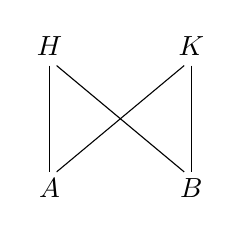
\begin{tikzpicture}[scale=0.9]
                \node [above] at (0,0) {$A$};
                \node [above] at (0,2) {$H$};
                \node [above] at (2,2) {$K$};
                \node [above] at (2,0) {$B$};
                \draw [-] (1.9,2) to (0.1,0.5);
                \draw [-] (2,2) to (2,0.5);
                \draw [-] (0,2) to (0,0.5);
                \draw [-] (0.1,2) to (1.9,0.5);
            \end{tikzpicture}
        \end{figure}
        But $A<H\cap K$, $B<H\cap K\Rightarrow A\vee B<H\cap K$. So $A\vee B\lhd H$, $A\vee B\lhd K$. That's contradictory! There is only one lower bound for $\{H,K\}$. Notice that $\{e\}<H\cap K$ so there exists at least one subgroup satisfies the condition. We have proved normality forms a lattice.
    \end{enumerate}
\end{answer}

$$ $$

\begin{ex}
    If $N_{1}\lhd G_{1}$, $N_{2}\lhd G_{2}$ then $(N_{1}\times N_{2})\lhd (G_{1}\times G_{2})$ and $(G_{1}\times G_{2})/(N_{1}\times N_{2})\cong (G_{1}/N_{1})\times(G_{2}/N_{2})$.
\end{ex}

\begin{answer}
    Take $a\in (N_{1}\times N_{2})$, $a=(n_{1},n_{2})$ where $n_{1}\in N_{1}$, $n_{2}\in N_{2}$. $\forall x\in (G_{1}\times G_{2})$, $x=(g_{1},g_{2})$ where $g_{1}\in G_{1}$, $g_{2}\in G_{2}$. $x^{-1}=(g_{1}^{-1},g_{2}^{-1})$, $x^{-1}ax=(g_{1}^{-1}n_{1}g_{1},g_{2}^{-1}n_{2}g_{2})$. $N_{1}\lhd G_{1}$, $N_{2}\lhd G_{2}$, so $g_{1}^{-1}n_{1}g_{1}\in N_{1}$, $g_{2}^{-1}n_{2}g_{2}\in N_{2}$. $x^{-1}ax\in (N_{1}\times N_{2})$. Thus $(N_{1}\times N_{2})\lhd (G_{1}\times G_{2})$.

    Assume $G_{1}=\bigcup\limits_{i\in I}N_{1}a_{i}$, $G_{2}=\bigcup\limits_{j\in J}N_{2}b_{j}$. Then $G_{1}\times G_{2}=\bigcup\limits_{i\in I}N_{1}a_{i}\times \bigcup\limits_{j\in J}N_{2}b_{j}$. Denote $A=\{a_{i}|i\in I\}$, $B=\{b_{j}|j\in J\}$. We construct two bijections $(G_{1}\times G_{2})/(N_{1}\times N_{2})\to A\times B$ and $(G_{1}/N_{1})\times(G_{2}/N_{2})$.\[f: N_{1}a_{i}\times N_{2}b_{j}\mapsto (a_{i},b_{j})\]\[g: (N_{1}a_{i}, N_{2}b_{j})\mapsto (a_{i},b_{j})\] Take $h=g^{-1}\circ f$, $f,g$ are bijections, so $h$ is an isomorphism. $(G_{1}\times G_{2})/(N_{1}\times N_{2})\cong (G_{1}/N_{1})\times(G_{2}/N_{2})$.
\end{answer}

$$ $$

\begin{ex}
    Let $N\lhd G$ and $K\lhd G$. If $N\cap K=\left\langle e\right\rangle$ and $N\vee K=G$, then $G/N\cong K$.
\end{ex}

\begin{answer}
    Assume $G=\bigcup\limits_{i\in I}Na_{i}$, we construct $f:k \to G /N$. We prove that $\forall x,y\in K$, $x,y$ belong to different cosets of $N$. Suppose not. $\exists x,y \in K$, $x,y\in Na_{i}$, then $xy^{-1}\in N\Rightarrow x=y$. That's contradictory! So $f$ is a monomorphism.

    $G=H\vee K$, so $G=HK$. we can write $x$ as $pq$, where $p\in H$, $q\in K$. $\left| G/H \right|=\left[G:H\right]=\left[HK:H\right]=\left[K:K\cap H\right]=\left| K \right| $. $f$ is a epimorphism.
    
    Thus, $G /N\cong K$.
\end{answer}

$$ $$

\begin{ex}
    If $f:G\to H$ is a homomorphism, $H$ is abelian and $N$ is a subgroup of $G$ containing $\mathrm{Ker}f$, then $N$ is normal in $G$.
\end{ex}

\begin{answer}
    Assume there exists $x\in G$, $x\notin N$ s.t. $f(x)\in f(N)$. $\exists n\in N$, $f(x)=f(n)$, $f(xn^{-1})=f(x)f(n)^{-1}=e'\Rightarrow xn^{-1}\in\mathrm{Ker}f\Rightarrow x\in N$. That's contradictory! $\forall x\in G$, $n\in N$, $f(x^{-1}nx)=f(x^{-1})f(n)f(x)=f(n)\in f(N)$, so $x^{-1}nx\in N$. Thus, $N\lhd G$.
\end{answer}

$$ $$

\begin{ex}
    \begin{enumerate}[(a)]
        \item Consider the subgroups $\left\langle 6\right\rangle$ and $\left\langle 30\right\rangle$ of $\mathbf{Z}$ and show that $\left\langle 6\right\rangle /\left\langle 30\right\rangle\cong Z_{5}$.
        \item For any $k,m>0$, $\left\langle k\right\rangle /\left\langle km\right\rangle\cong Z_{m}$; in particular, $\mathbf{Z}/\left\langle m\right\rangle=\left\langle 1\right\rangle /\left\langle m\right\rangle\cong Z_{m}$.
    \end{enumerate}
\end{ex}

\begin{answer}
    \begin{enumerate}[(a)]
        \item $\left\langle 6\right\rangle=\{6n|n\in \mathbf{Z}\}$, $\left\langle 30\right\rangle=\{30n|n\in \mathbf{Z}\}$. So $\left\langle 6\right\rangle/\left\langle 30\right\rangle=\{\left\langle 30\right\rangle, \left\langle 30\right\rangle +6, \left\langle 30\right\rangle +12, \left\langle 30\right\rangle +18, \left\langle 30\right\rangle +24\}\cong Z_{5}$
        \item $\left\langle km\right\rangle\lhd \left\langle k\right\rangle$, $\left\langle k\right\rangle=\bigcup\limits_{i\in I}(\left\langle km\right\rangle +a_{i})$. For $x\in \left\langle k\right\rangle$, $x\equiv a_{i}\mod km$, then $x\in \left\langle km \right\rangle +a_{i}$. $f:\left\langle k\right\rangle/\left\langle km\right\rangle\to \{a_{i}|i\in I\}$ defined by $f(\left\langle km\right\rangle +a_{i})=a_{i}$ is a bijection. We check that $g: \{a_{i}|i\in I\}\to Z_{m}$ is also a bijection. Define $b_{i}\equiv \frac{a_{i}}{k}\mod m$, $g(a_{i})=b_{i}$. If there exists $b_{i}=b_{j}$ for $i\neq j$, $a_{i}\equiv a_{j}\mod km$. That's contradictory! So $g$ is an injection. $g$ is obviously a surjection, so $g$ is a bijection. Take $h= g\circ f:\left\langle k\right\rangle /\left\langle km \right\rangle\to Z_{m}$ is a isomorphism, so $\left\langle k\right\rangle /\left\langle km \right\rangle\cong Z_{m}$.
    \end{enumerate}
\end{answer}

$$ $$

\begin{ex}
    If $f: G \to H$ is a homomorphism with kernel $N$ and $K<G$, then prove that $f^{-1}(f(K))=KN$. Hence $f^{-1}(f(K))=K$ if and only if $N<K$.
\end{ex}

\begin{answer}
    Take $x\in f^{-1}(f(K))$, then there exists $k\in K$ s.t. $f(x)=f(k)$. $f(xk^{-1})=f(x)f(k)^{-1}=e'\in f(K) \Rightarrow xk^{-1}\in\mathrm{Ker}f=N$. Thus, $x\in Nk\subset NK$, $f^{-1}(f(K))\subset NK$.

    $\forall x=nk\in NK$, where $n\in N$ and $k\in K$. $f(x)=f(n)f(k)=e'f(k)\in f(K)$, so $NK\subset f^{-1}(f(K))$.

    Thus, $f^{-1}(f(K))=NK$. Hence $f^{-1}(f(K))=K$ if and only if $N<K$.
\end{answer}

$$ $$

\begin{ex}
    If $N\lhd G$, $\left[G:H\right]$ finite, $H<G$, $\left| H \right| $ finite, and $\left[G:N\right]$ and $\left| H \right| $ are relatively prime, then $H<N$.
\end{ex}

\begin{answer}
    $N\lhd G\Rightarrow NH<G$. By the second isomorphism theorem, $NH /N\cong H/H\cap N\Rightarrow \left[NH:N\right]=\left[H:H\cap N\right]$. Assume $\left[G:N\right]=m$, $\left| H \right| =n$, $\left| G \right| =mnp$ where $(m,n)=1$. Then $\left| N \right| =np$, $N<NH$, assume $\left| NH \right| =knp$, $NH<G\Rightarrow knp|mnp\Rightarrow k|m$. $\left[NH:N\right]=\left[H:H\cap N\right]=k\Rightarrow k|n$. So $k=1$, $NH=N$ which means $H<N$.
\end{answer}

$$ $$

\begin{ex}
    If $N\lhd G$, $\left| N \right|$ finite, $H<G$, $\left[G:N\right] $ finite, and $\left[G:H\right]$ and $\left| N \right| $ are relatively prime, then $N<H$.
\end{ex}

\begin{answer}
    $N\lhd G\Rightarrow NH<G$. By the second isomorphism theorem, $NH /N\cong H/H\cap N\Rightarrow \left[NH:N\right]=\left[H:H\cap N\right]$. Assume $\left[G:H\right]=m$, $\left| N \right| =n$, $\left| G \right| =mnp$ where $(m,n)=1$. Then $\left| H \right| =np$, $H<NH$, assume $\left| NH \right| =knp$, $NH<G\Rightarrow knp|mnp\Rightarrow k|m$. $\left[NH:N\right]=\left[H:H\cap N\right]=kp\Rightarrow kp|np\Rightarrow k|n$. So $k=1$, $NH=H$ which means $N<H$.
\end{answer}

$$ $$

\begin{ex}
    If $H$ is a subgroup of $Z(p^{\infty})$ and $H\neq Z(p^{\infty})$, then $Z(p^{\infty}) /H\cong Z(p^{\infty})$.
\end{ex}

\begin{answer}
    From \textbf{Exercise 1.3.7}(b), we know that $H$ has the form $\left\langle \bar{\frac{1}{p^{n}}}\right\rangle$. Take $x_{i}=\bar{\frac{1}{p^{n+i}}}+H$, $x_{1}=\bar{\frac{1}{p^{n+1}}}+H$. \[\sum_{m=1}^{p}x_{1}=\bar{\frac{p}{p^{n+1}}}+pH=\bar{\frac{1}{p^{n}}}+H=H\] \[\sum_{m=1}^{p}x_{i}=\bar{\frac{p}{p^{n+i}}}+pH=\bar{\frac{1}{p^{n+i-1}}}+H=x_{i-1}\] Take $A=\{x_{i}|i\in \mathbf{Z}_{+}\}$, $\left\langle A\right\rangle\cong Z(p^{\infty})$ by \textbf{Exercise 1.3.7}(e). $\forall x\in \left\langle A\right\rangle$, $x\in Z(p^{\infty}) /H$, so $\left\langle A\right\rangle\subset Z(p^{\infty}) /H$. Take $x\in Z(p^{\infty}) /H$, $x=y+H$ where $y=\sum\limits_{i=1}^{m}\frac{a_{i}}{p^{n+i}}$, $x=\sum\limits_{i=1}^{m}(\frac{a_{i}}{p^{n+i}}+H)\in \left\langle A\right\rangle$. Thus, $Z(p^{\infty}) /H\subset \left\langle A\right\rangle$, $\left\langle A\right\rangle=Z(p^{\infty}) /H\cong Z(p^{\infty})$.
\end{answer}
\section{Symmetric, alternating, and dihedral groups}
\begin{ex}
    Find four different subgroups of $S_{4}$ that are isomorphic to $S_{3}$ and nine isomorphic to $S_{2}$.
\end{ex}

\begin{answer}
    $S_{4}=\{(1), (12), (13), (14), (23), (24), (34), (123), (124), (132),\\ (142), (134), (143), (234), (243), (12)(34), (13)(24), (14)(23), (1234),\\ (1243), (1324), (1342), (1423), (1432)\}$.

    $A_{1}=\{(1), (12), (13), (23), (123), (132)\}$;

    $A_{2}=\{(1), (12), (14), (24), (124), (142)\}$;

    $A_{3}=\{(1), (13), (14), (34), (134), (143)\}$;

    $A_{4}=\{(1), (23), (24), (34), (234), (243)\}$;
    
    $A_{1}\cong A_{2}\cong A_{3}\cong A_{4}$.

    $B_{1}=\{(1), (12)\}$; $B_{2}=\{(1),(13)\}$; $B_{3}=\{(1),(14)\}$; $B_{4}=\{(1), (23)\}$; $B_{5}=\{(1),(24)\}$; $B_{6}=\{(1), (34)\}$; $B_{7}=\{(1),(12)(34)\}$; $B_{8}=\{(1),(13)(24)\}$; $B_{9}=\{(14)(23)\}$;

    $B_{1}\cong B_{2}\cong B_{3}\cong B_{4}\cong B_{5}\cong B_{6}\cong B_{7}\cong B_{8}\cong B_{9}$.
\end{answer}

$$ $$

\begin{ex}
    \begin{enumerate}[(a)]
        \item $S_{n}$ is generated by the $n-1$ transpositions $(12)$, $(13)$, $(14)$, $\dots$, $(1n)$.
        \item $S_{n}$ is generated by the $n-1$ transpositions $(12), (23), (34),\dots, (n-1\, n)$.
    \end{enumerate}
\end{ex}

\begin{answer}
    \begin{enumerate}[(a)]
        \item $\forall x\in S_{n}$, $x$ can be written as a product of transpositions. Actually, for any transposition $(ij)$, we can obtain it by $(1i)(1j)(1i)=(ij)$. So $x\in \left\langle (12), (13),\dots,(1n)\right\rangle$, $S_{n}\subset\left\langle(12), (13),\dots,(1n)\right\rangle$.
        \item We can contruct $(1i)$ inductively since $(1i)=(1\, i-1)(i-1\, i)(1\, i-1)$. From (a), we have $\forall x\in S_{n}$, $x\in \left\langle (12), (13),\dots,(1n)\right\rangle$. Thus $S_{n}\subset\left\langle(12), (13),\dots,(1n)\right\rangle\subset \left\langle (12), (23), (34),\dots, (n-1\, n)\right\rangle$.
    \end{enumerate}
\end{answer}

$$ $$

\begin{ex}
    If $\sigma=(i_{1}i_{2}\cdots i_{r})\in S_{n}$ and $\tau\in S_{n}$, then $\tau\sigma\tau^{-1}$ is the $r$-cycle $(\tau(i_{1})\tau(i_{2})\cdots\tau(i_{r}))$.
\end{ex}

\begin{answer}
    $\sigma(i_{n})=i_{n+1}$ for $n=1,2,\dots,r-1$, $\sigma(i_{r})=i_{1}$. Assume $\tau(i_{n})=j_{n}$, $n=1,2,\dots,r-1$ and $I=\{i_{n}|n=1,2,\dots,r-1\}$, $J=\{j_{n}|n=1,2,\dots,r-1\}$. For $x\notin J$, $\tau\sigma\tau^{-1}(x)=\tau\tau^{-1}(x)=x$. For $x=j_{k}\in J$, $\tau^{-1}(x)=i_{k}$, $\sigma(\tau^{-1}(x))=i_{k+1}$, $\tau(\sigma(\tau^{-1}(x)))=j_{k+1}$ and $\tau\sigma\tau^{-1}(j_{r})=j_{1}$. Thus $\tau\sigma\tau^{-1}=(\tau(i_{1})\tau(i_{2})\cdots\tau(i_{r}))$.
\end{answer}

$$ $$

\begin{ex}
    \begin{enumerate}[(a)]
    \item $S_{n}$  is generated by $\sigma_{1}=(12)$ and $\tau=(123\cdots n)$.
    \item $S_{n}$ is generated by $(12)$ and $(23\cdots n)$.
    \end{enumerate}
\end{ex}

\begin{answer}
    \begin{enumerate}[(a)]
        \item Denote $\sigma_{i}=\tau\sigma_{i-1}\tau^{-1}$. Applying \textbf{Exercise 1.6.3}, $\sigma_{i}=(i\, i+1)$. By \textbf{Exercise 1.6.2}(b), $S_{n}\subset\left\langle (12), (23), (34),\dots, (n-1\, n)\right\rangle=\left\langle\sigma_{1}, \sigma_{2},\dots,\sigma_{n-1}\right\rangle\subset \left\langle \tau, \sigma_{1}\right\rangle$. $S_{n}$ can be generated by $\tau$ and $\sigma_{1}$.
        \item Denote $\sigma_{1}=(12)$, $\tau=(23\cdots n)$, $\sigma_{i}=\tau\sigma_{i-1}\tau^{-1}$. Applying \textbf{Exercise 1.6.3},$\sigma_{i}=(1\, i+1)$. By \textbf{Exercise 1.6.2}(a), $S_{n}\subset\left\langle(12), (13),\dots,(1n)\right\rangle=\left\langle \sigma_{1},\sigma_{2},\dots,\sigma_{n-1}\right\rangle\subset\left\langle \tau,\sigma_{1}\right\rangle$. $S_{n}$ can be generated by $\tau$ and $\sigma_{1}$.
    \end{enumerate}
\end{answer}

$$ $$

\begin{ex}
    Let $\sigma, \tau \in S_{n}$. If $\sigma$ is even (odd), then so is $\tau\sigma\tau^{-1}$.
\end{ex}

\begin{answer}
    Assume $\sigma=(x_{1}x_{2})\cdots(x_{2n-1}x_{2n})$, $\tau=(y_{1}y_{2})\cdots(y_{2m-1}y_{2m})$. Then $\tau^{-1}=(y_{2m-1}y_{2m})\cdots(y_{1}y_{2})$. $\sigma$ is odd (even) if an only if $n$ is odd (even). $\tau\sigma\tau^{-1}$ has $2m+n$ transpositions. We can add $(ij)=(ji)=(1)$ into some segments of $\tau\sigma\tau^{-1}$ without changing it. So $\tau\sigma\tau^{-1}$ is odd (even) if and only if $2m+n$ is odd (even). $2m+n\equiv n\mod 2$ so $\tau\sigma\tau^{-1}$ is odd (even) if and only if $\sigma$ is odd (even).
\end{answer}

$$ $$

\begin{ex}
    $A_{n}$ is the only subgroup of $S_{n}$ of index 2.
\end{ex}

\begin{answer}
    For any subgroup $N<S_{n}$ and $\left[S_{n}:N\right]=2$, we have $N\lhd S_{n}$.

    Assume there exists $k$-circle $\sigma=(i_{1}i_{2}\cdots i_{k})\in N$. Then for any other $k$-circle $(j_{1}j_{2}\cdots j_{k})$, take $\tau=(i_{i}j_{1})(i_{2}j_{2})\cdots(i_{k}j_{k})$, by \textbf{Exercise 1.6.3}, $\tau\sigma\tau^{-1}=(j_{1}j_{2}\cdots j_{k})\in N$. Thus $N$ contains all the $k$-circles.

    For $n\geq 5$. If there exists 3-circle in $N$, then all the 3-circles are contained in $N$, $A_{n}\subset N\subset S_{n}\Rightarrow A_{n}=N$.

    If there exists 2-circle in $N$, then all the 2-circles are contained in $N$. Notice $(1i)(1j)=(1ij)\in N$ is a 3-circle, so $A_{n}=N$.

    If there only contain $x$ in the form of $(a_{i}a_{2}\cdots a_{n_{1}})(b_{1}b_{2}\cdots b_{n_{2}})\cdots$ where $n_{i}\geq 4$ and every two circles are disjoint. Take $\tau_{i}:\{a_{i}|i=1,2,\dots,n_{1}\}\to \{a_{i}|i=1,2,\dots,n_{1}\}$. We can obtain product of two $n_{1}$-circles\[x^{-1}\tau x \tau^{-1}=(a_{1}a_{2}\cdots a_{n_{1}})(\tau(a_{1})\tau(a_{2})\cdots \tau(a_{n}))\in N\] By the arbitrariness of $\tau$, take \[(\tau(a_{1})\tau(a_{2})\cdots \tau(a_{n}))=(a_{1}a_{4}a_{5}\cdots a_{n}a_{3}a_{2})\] then $x^{-1}\tau x \tau^{-1}=(a_{1}a_{3})(a_{2}a_{4})$ is a product of 2-circles. We can take $a_{1}, a_{2}, a_{3}, a_{4}$ arbitrarily. WLOG, take $(12)(34)\in N$ and $(12)(35)\in N$, $(12)(35)(12)(34)=(345)\in N$. Then there exists 3-circle in $N$, $N=A_{n}$.

    In conlusion, when $n\geq 5$, $S_{n}$ has only one normal subgroup $A_{n}$.

    For $n=2,3,4$, we can verify it by enumeration.
\end{answer}

$$ $$

\begin{ex}
    Show that $N=\{(1),(12)(34),(13)(24),(14)(23)\}$ is a normal subgroup of $S_{4}$ contained in $A_{4}$ such that $S_{4} /N\cong S_{3}$ and $A_{4} /N\cong Z_{3}$.
\end{ex}

\begin{answer}
    Assume $\sigma=(i_{1}i_{2})(i_{3}i_{4})\in N$, $\forall \tau\in S_{4}$, $\tau(i_{n})=j_{n}$, $J=\{j_{n}|n=1,2,3,4\}$. For $x\notin J$, $\tau\sigma\tau^{-1}(x)=\tau\tau^{-1}(x)=x$. For $x=j_{k}\in J$, $\tau^{-1}(x)=i_{k}$, $\sigma\tau^{-1}(x)=i_{3k-4\left[\frac{k}{2}\right]-1}$, $\tau\sigma\tau^{-1}(x)=(\tau(i_{i})\tau(i_{2}))(\tau(i_{3})\tau(i_{4}))\in N$. So $N\lhd S_{4}$. $S_{4} /N=\{N, N(12), N(13), N(23), N(123), N(132)\}\cong S_{3}$. $A_{4} /N=\{N, N(123), N(132)\}\cong Z_{3}$.
\end{answer}

$$ $$

\begin{ex}
    The group $A_{4}$ has no subgroup of order $6$.
\end{ex}

\begin{answer}
    $\left| A_{4} \right| =12$, assume there exists $N<A_{4}$, $\left| N \right| =6$. Then $N\lhd A_{4}$. From \textbf{Exercise 1.6.6}, we know that all 3-circles are contained in $N$. But there're 8 3-circles in total, so $N$ can't exist.
\end{answer}

$$ $$

\begin{ex}
    For $n\geq 3$ let $G_{n}$ be the multiplicaive group of complex matrices generated by $x=\begin{pmatrix}
        0&1\\1&0
    \end{pmatrix}$ and $y=\begin{pmatrix}
        e^{2\pi i/n}&0\\0&e^{-2\pi i/n}
    \end{pmatrix}$, where $i^{2}=-1$. Show that $G_{n}\cong D_{n}$.
\end{ex}

\begin{answer}
    Take a mapping $f:G_{n}\to D_{n}$ as $f(x)=(2\,n)(3\,n-1)\cdots$, $f(y)=(123\cdots n)$. $\left| f(x) \right|=\left| x \right| =2$, $\left| f(y) \right| =\left| y \right| =n$. $f$ is obviously a monomorphism. $\forall a\in D_{n}$, $a=f(x)^{n}f(y)^{m}, m=1,2$, then $a=f(x^{n}y^{m})$, $f$ is a epimorphism. Thus $G_{n}\cong D_{n}$. 
\end{answer}

$$ $$

\begin{ex}
    Let $a$ be the generator of order $n$ of $D_{n}$. Show that $\left\langle a\right\rangle\lhd D_{n}$ and $D_{n} /\left\langle a\right\rangle\cong Z_{2}$.
\end{ex}

\begin{answer}
    $\left| \left\langle a\right\rangle \right| =n$, $b$ is the other generator of $D_{n}$, $a^{n}=b^{2}=(1)$. $\forall k\in \mathbf{Z}$, $a^{k}b=ba^{-k}$ can be easily proved by induction. So $\forall x=a^{m}b^{n}\in D_{n}$, $x=a^{m'}b^{n'}$, here $m'\equiv m\mod 2$, $n'\equiv n\mod 2$. $D_{n}=\{e, a, a^{2}, \dots, a^{n-1}, b, ba, \\\dots, ba^{n-1}\}$. $\left| D_{n} \right| =2n$. Thus, $\left\langle a\right\rangle\lhd D_{n}$. $D_{n} /\left\langle a\right\rangle=\{\left\langle a\right\rangle, \left\langle a\right\rangle b\}\cong Z_{2}$.
\end{answer}

$$ $$

\begin{ex}
    Find all normal subgroups of $D_{n}$.
\end{ex}

\begin{answer}
    The subgroups of $\left\langle a\right\rangle$ is always normal in $D_{n}$. $\left\langle a^{m}\right\rangle <\left\langle a\right\rangle$. $\forall x\in D_{n}$ and $a^{km}\in \left\langle a^{m}\right\rangle$, $x=a^{t}$ or $x=ba^{t}$. \[x^{-1}a^{km}x=a^{-t}a^{km}a^{t}=a^{km}\in\left\langle a^{m}\right\rangle\] or \[x^{-1}a^{km}x=a^{-t}b^{-1}a^{km}ba^{t}=a^{-t}ba^{km}ba^{t}=a^{-t}a^{-km}b^{2}a^{t}=a^{-km}\in \left\langle a^{m}\right\rangle\] so $\left\langle a^{m}\right\rangle \lhd D_{n}$.

    Consider the subgroup $S$ which only contains $ba^{i}, i=1,\dots, n$. Since $ba^{i}\cdot ba^{j}=a^{j-i}\in S\,(i\neq j)$, so $S=\{e, ba^{k}\}$.

    If $n$ is odd, take $x=a^{\frac{n-1}{2}}\in D_{n}$. \[x^{-1}ba^{k}x=a^{\frac{1-n}{2}}ba^{k}a^{\frac{n-1}{2}}=ba^{k+n-1}\notin S\] so $S\ntriangleleft D_{n}$ for all $k=1,2,\dots,n$.

    If $n$ is even, take $x=a^{\frac{n-2}{2}}\in D_{n}$, $n\geq 6$. \[x^{-1}ba^{k}x=a^{\frac{2-n}{2}}ba^{k}a^{\frac{n-2}{2}}=ba^{k+n-2}\notin S\] so $S\ntriangleleft D_{n}$ for all $k=1,2,\dots,n$.

     If $n=2$, all the subgroups are normal since $\left| D_{2} \right| =4$.

     For subgroup $S$ contains both $ba^{i}$ and $a^{j}$. It can be written as $S=\left\langle a^{d}, ba^{r}\right\rangle$, where $d|n$, $0\leq r\leq d-1$. If $\exists a^{m}, a^{n}\in S$, $(m,n)=d$, then there exist $x,y\in \mathbf{Z}$ s.t. $a^{mx+ny}=a^{d}\in \mathbf{Z}$. Thus, $S=\left\langle a^{d},ba^{r}\right\rangle$.

     Take $x=a^{\frac{n-w}{2}}$, then $x^{-1}ba^{r}x=ba^{r+n-w}$.
     
     If $d\geq 3$, take $w\equiv n\mod 2$, $x^{-1}ba^{r}x\notin S$.

     If $d=2$, then $n=2s$ and $S=\{e, a^{s}, ba^{s}, b\}$. $Sa^{k}=\{a^{k}, a^{s+k},ba^{s-k}, ba^{-k}\}$, $k=1,2,\dots, s-1$. $ba^{k}=ba^{-k}$ or $ba^{k}=ba^{s-k}\Rightarrow k=\frac{s}{2}$. So for $s=2$, $n=4$, $S$ is a normal subgroup of $D_{4}$.
\end{answer}

$$ $$

\begin{ex}
    The center of the group $D_{n}$ is $\left\langle e\right\rangle$ if $n$ is odd and isomorphic to $Z_{2}$ if $n$ is even.
\end{ex}

\begin{answer}
    If $n$ is odd, $C$ is the center of $D_{n}$, $C\lhd D_{n}\Rightarrow C<\left\langle a\right\rangle$. Take $a^{d}\in C$, $x=ba^{m}$, \[x^{-1}ax=a^{-m}b^{-1}a^{d}ba^{m}=a^{-m}ba^{d}ba^{m}=a^{-d}=a^{d}\] so $d=0$, $C=\{e\}$.

    If $n$ is even, $n\geq 6$. $C$ is the center of $D_{n}$. $C\lhd D_{n}\Rightarrow C<\left\langle a\right\rangle$ or $C=\{e,ba^{k}\}$.
    
    If $C=\{e,ba^{k}\}$, $C\cong Z_{2}$.
    
    If $C<\left\langle a\right\rangle$,take $a^{d}\in C$, $x=ba^{m}$, \[x^{-1}ax=a^{-m}b^{-1}a^{d}ba^{m}=a^{-m}ba^{d}ba^{m}=a^{-d}=a^{d}\] so $d=\frac{n}{2}$ or $d=0$, $C=\{a^{\frac{n}{2}},e\}\cong Z_{2}$.
\end{answer}

$$ $$

\begin{ex}
    For each $n\geq 3$ let $P_{n}$ be a regular polygon of $n$ sides (for $n=3$, $P_{n}$ is an equilateral triangle; for $n=4$, a square). A \emph{symmetry} of $P_{n}$ is a bijection $P_{n}\to P_{n}$ that preserves distances and maps adjacent vertices on to adjacent vertices.
    
    \begin{enumerate}[(a)]
        \item The set $D_{n}^{*}$ of all symmetries of $P_{n}$ is a group under the binary operation of composition of functions.
        \item Every $f\in D_{n}^{*}$ is completely determined by its actions on the vertices of $P_{n}$. Number the vertices consecutively $1,2,\dots, n$; then each $f\in D_{n}^{*}$ determines a unique permutation $\sigma_{f}$ of $\{1,2,\dots, n\}$. The assignment $f\mapsto \sigma_{f}$ defines a monomorphism of groups $\varphi:D_{n}^{*}\to S_{n}$.
        \item $D_{n}^{*}$ is generated by $f$ and $g$, where $f$ is a rotation of $2\pi /n$ degrees about the center of $P_{n}$ and $g$ is a reflection about the ``diameter'' through the center and vertex 1.
        \item $\sigma_{f}=(123\cdots n)$ and $\sigma_{g}=\begin{pmatrix}
            1&2&3&\cdots&n-1&n\\1&n&n-1&\cdots&3&2
        \end{pmatrix}$, whence \\$\mathrm{Im}\varphi=D_{n}$ and $D_{n}^{*}\cong D_{n}$.
    \end{enumerate}
\end{ex}

\begin{answer}
    In the following analysis, all the numbers are $\mod n$.
    \begin{enumerate}[(a)]
        \item Consider $n$ points $A_{i}=(\cos \frac{2\pi i}{n},\sin \frac{2\pi i}{n})^{t}$, $i=1,2,\dots,n$. $f$ is the transposition of $A_{i}\mapsto A_{j}$ with the consevation of $n$ regular polygon structure. So $f$ must be a bijection. $D_{n}^{*}$ is the set of $f$. By the definition, $D_{n}^{*}\subset S_{n}$. We prove $D_{n}^{*}$ is ta subgroup of $S_{n}$.
        
        Notice that $A_{i+1}=\begin{pmatrix}
            \cos \frac{2\pi i}{n}&-\sin\frac{2\pi i}{n}\\\sin\frac{2\pi i}{n}&\cos \frac{2\pi i}{n}
        \end{pmatrix}A_{i}$.
        
        Denote $X=\begin{pmatrix}
            \cos \frac{2\pi i}{n}&-\sin\frac{2\pi i}{n}\\\sin\frac{2\pi i}{n}&\cos \frac{2\pi i}{n}
        \end{pmatrix}$. To construct the polygon,  we must have \[f(A_{i+1})=\begin{pmatrix}
            \cos \frac{2\pi i}{n}&-\sin\frac{2\pi i}{n}\\\sin\frac{2\pi i}{n}&\cos \frac{2\pi i}{n}
        \end{pmatrix}f(A_{i})\] or \[f(A_{i})=\begin{pmatrix}
            \cos \frac{2\pi i}{n}&-\sin\frac{2\pi i}{n}\\\sin\frac{2\pi i}{n}&\cos \frac{2\pi i}{n}
        \end{pmatrix}f(A_{i+1})\] We need to verify that $\forall f_{1}, f_{2}\in D_{n}^{*}$, $f_{1}f_{2}^{-1}\in D_{n}^{*}$. Assume $B_{i}=f_{2}(A_{i})$, $B_{i+1}=f_{2}(A_{i+1})$. Then $B_{i}=XB_{i+1}$ or $B_{i}=X^{-1}B_{i+1}$. Denote $B_{i}=A_{j}$, then $B_{i+1}=A_{j-1}$ or $B_{i+1}=A_{j+1}$. WLOG, assume $B_{i+1}=A_{j+1}$, then $f_{1}(A_{j})=Xf_{1}(A_{j+1})$ or $f_{1}(A_{j})=X^{-1}f_{1}(A_{j-1})$. So $f_{1}f_{2}^{-1}\in D_{n}^{*}$. $D_{n}^{*}$ is a subgroup of $S_{n}$.
        \item Assume $A_{i}=f(A_{1})$. If $f(A_{2})=A_{i+1}$, since $f$ is a bijection, by induction, we can prove $f(A_{k})=A_{k+i-1}$. $\varphi: D_{n}^{*}\to S_{n}$ can be defined as $\varphi: f\mapsto (1i\,2i-1\,3i-2\cdots)$. If $f(A_{2})=A_{i-1}$, similarly, we can also prove $f(A_{k})=A_{i+1-k}$. $\varphi$ can be defined as $\varphi: f\mapsto (1i)(2\,i-1)(3\,i-2)\cdots$. This means $f$ is completely determined by $f(A_{1})$ and $f(A_{2})$. $D_{n}^{*}$ can be embedded into $S_{n}$.
        \item Denote $\alpha=\begin{pmatrix}
            \cos \frac{2\pi i}{n}&-\sin\frac{2\pi i}{n}\\\sin\frac{2\pi i}{n}&\cos \frac{2\pi i}{n}
        \end{pmatrix}$, $\beta=\begin{pmatrix}
            1&0\\0&1
        \end{pmatrix}$. $f:A_{i}\mapsto \alpha A_{i}$, $g:A_{i}\mapsto \beta A_{i}$. $f$ is the rotation of $\frac{2\pi}{n}$ degrees counter-clockwisely. $g$ is the reflection about $x$-axis. Now we prove $\forall x\in D_{n}^{*}$, $x$ can be factorised into finite product of $f$ and $g$. From (b), $x$ is fully defined by $x(A_{1})$ and $x(A_{2})$. Assume $x(A_{1})=A_{i}$.

        If $x(A_{2})=A_{i+1}$, $x(A_{k})=A_{i-1+k}=\alpha^{i-1}A_{k}$, $k=1,2,\dots,n$. So $x=f^{i-1}$.

        If $x(A_{2})=A_{i-2}$, $x(A_{k})=A_{i+1-k}=\alpha^{i+1}A_{-k}=\alpha^{i+1}\beta A_{k}$. So $x=f^{i+1}g$. Thus $D_{4}^{*}\subset\left\langle f,g\right\rangle$.
        \item $\alpha^{n}=\beta^{2}=\begin{pmatrix}
            1&0\\0&1
        \end{pmatrix}$. We can easily verify that $\left| f \right| =n$ and $\left| g \right| =2$. From \textbf{Exercise 1.6.9}, $\left\langle f,g\right\rangle\cong D_{n}$, $\left| \left\langle f,g\right\rangle \right| =\left| D_{n} \right| =2n$. From (b), $x\in D_{n}^{*}$ if completely determined by $x(A_{1})$ and $x(A_{2})$. There are $2n$ different ways to obtain $x(A_{1})$ and $x(A_{2})$. So $\left| D_{n}^{*} \right| =\left| \left\langle f,g\right\rangle \right| =2n$. $D_{n}^{*}\subset \left\langle f,g\right\rangle$, so $D_{n}^{*}=\left\langle f,g\right\rangle$. Thus, $D_{n}^{*}\cong \left\langle f,g\right\rangle\cong D_{n}$.
    \end{enumerate}
\end{answer}
\section{Categories: products, coproducts, and free objects}
\begin{ex}
    A \emph{pointed set} is a pair $(S,x)$ with $S$ a set and $x\in S$. A morphism of pointed sets $(S,x)\to (S', x')$ is a triple $(f,x,x')$, where $S\to S'$ is a function such that $f(x)=x'$. Show that pointed sets form a category.
\end{ex}

\begin{answer}
    Let $\mathcal{S}$ be the category and 4 objects of $\mathcal{S}$ are $(A,a)$, $(B,b)$, $(C,c)$, $(D,d)$. $f$, $g$ and $h$ are morphisms defined by $f:A\to B$, $g:B\to C$, $h:C\to D$ with $f(a)=b$, $g(b)=c$, $h(c)=d$.

    \begin{figure}[H]\centering
        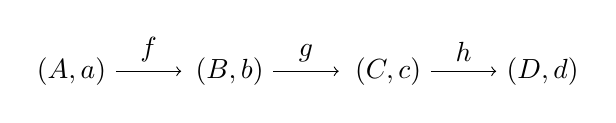
\begin{tikzpicture}
            \node [left] at (0,1) {$(A,a)$};
            \node [left] at (2,1) {$(B,b)$};
            \node [left] at (4,1) {$(C,c)$};
            \node [left] at (6,1) {$(D,d)$};
            \draw [->] (0,1)-- node [above, pos=0.5]{$f$}(0.83,1);
            \draw [->] (2,1)-- node [above, pos=0.5]{$g$}(2.83,1);
            \draw [->] (4,1)-- node [above, pos=0.5]{$h$}(4.83,1);
        \end{tikzpicture}
        \caption*{category $\mathcal{S}$}
    \end{figure}
    \[\mathrm{hom}(A,B)\times\mathrm{hom}(B,C)\to \mathrm{hom}(A,C)\]because $g\circ f:A\to C$ with $g(f(a))=g(b)=c=g\circ f(a)$. Similarly, $(h\circ g)\circ f=h\circ (g\circ f)$ with $(h\circ g)\circ f(a)=h\circ (g\circ f)(a)=d$. Take $1_{B}$ consist of those functions $i:B\to B$ with $i(b)=b$. Then $1_{B}\circ f=f$ and $g\circ 1_{B}=g$. So $\mathcal{S}$ is a category.
\end{answer}

$$ $$

\begin{ex}
    If $f:A\to B$ is an equivalence in a category $\mathcal{C}$ and $g:B\to A$ is the morphism such that $g\circ f=1_{A}$, $f\circ g=1_{B}$, show that $g$ is unique.
\end{ex}

\begin{answer}
    Assume there exist $g$ and $g'$ satisfies the condition.

    \begin{figure}[H]\centering
        \subfigure{
            \begin{minipage}[c]{0.3\linewidth}
                \centering
                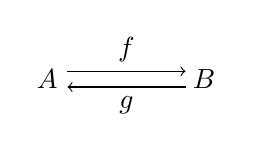
\begin{tikzpicture}
                    \node [left] at (0,1) {$A$};
                    \node [left] at (2,1) {$B$};
                    \draw [->] (0,1.1)-- node [above, pos=0.5]{$f$} (1.5,1.1);
                    \draw [<-] (0,0.9)-- node [below, pos=0.5]{$g$} (1.5,0.9);
                \end{tikzpicture}
            \end{minipage}
        }
        \subfigure{
            \begin{minipage}[c]{0.3\linewidth}
                \centering
                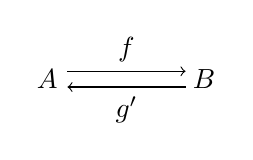
\begin{tikzpicture}
                    \node [left] at (0,1) {$A$};
                    \node [left] at (2,1) {$B$};
                    \draw [->] (0,1.1)-- node [above, pos=0.5]{$f$} (1.5,1.1);
                    \draw [<-] (0,0.9)-- node [below, pos=0.5]{$g'$} (1.5,0.9);
                \end{tikzpicture}
            \end{minipage}
        }
    \end{figure}
    So $g'\circ(f\circ g)=g'\circ 1_{B}=g'=(g'\circ f)\circ g=1_{A}\circ g =g$.
\end{answer}

$$ $$

\begin{ex}
    In the category $\mathcal{G}$ of groups, show that the group $G_{1}\times G_{2}$ together with the homomorphisms $\pi_{1}:G_{1}\times G_{2}\to G_{1}$ and $\pi_{2}:G_{1}\times G_{2}\to G_{2}$ is a product for $\{G_{1},G_{2}\}$.
\end{ex}

\begin{answer}
    Take $\tau_{1}:G_{1}\to G_{1}\times G_{2}$ as $\tau_{1}(g_{1})=(g_{1},e)$; $\tau_{2}:G_{2}\to G_{1}\times G_{2}$ as $\tau_{2}(g_{2})=(e,g_{2})$; $\pi_{1}:G_{1}\times G_{2}\to G_{1}$ as $\pi_{1}(g_{1},g_{2})=g_{1}$; $\pi_{2}:G_{1}\times G_{2}\to G_{2}$ as $\pi_{2}(g_{1},g_{2})=g_{2}$. Then

    \begin{figure}[H]\centering
        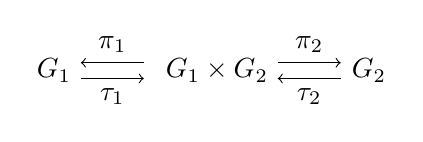
\begin{tikzpicture}
            \node [left] at (0,1) {$G_{1}$};
            \node [left] at (2.5,1) {$G_{1}\times G_{2}$};
            \node [left] at (4,1) {$G_{2}$};
            \draw [<-] (0,1.1)-- node [above, pos=0.5]{$\pi_{1}$} (0.8,1.1);
            \draw [->] (0,0.9)-- node [below, pos=0.5]{$\tau_{1}$} (0.8,0.9);
            \draw [->] (2.5,1.1)-- node [above, pos=0.5]{$\pi_{2}$} (3.3,1.1);
            \draw [<-] (2.5,0.9)-- node [below, pos=0.5]{$\tau_{2}$} (3.3,0.9);
        \end{tikzpicture}
    \end{figure}
    For any object $B$ such that

    \begin{figure}[H]\centering
        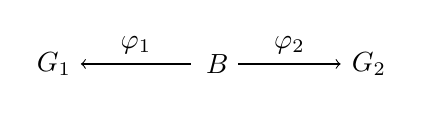
\begin{tikzpicture}
            \node [left] at (0,1) {$G_{1}$};
            \node [left] at (2,1) {$B$};
            \node [left] at (4,1) {$G_{2}$};
            \draw [<-] (0,1)-- node [above, pos=0.5]{$\varphi_{1}$} (1.4,1);
            \draw [->] (2,1)-- node [above, pos=0.5]{$\varphi_{2}$} (3.3,1);
        \end{tikzpicture}
    \end{figure}
    For any $x\in B$, define $f:B\to G_{1}\times G_{2}$ as $f(x)=(\varphi_{1}(x), \varphi_{2}(x))$. Then $\pi_{1}(f(x))=\varphi_{1}(x)$, $\pi_{1}\circ f=\varphi_{1}$, $\pi_{2}(f(x))=\varphi_{2}(x)$, $\pi_{2}\circ f=\varphi_{2}$. Thus
    
    \begin{figure}[H]\centering
        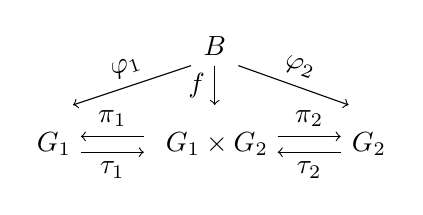
\begin{tikzpicture}
            \node [left] at (0,1) {$G_{1}$};
            \node [left] at (2.5,1) {$G_{1}\times G_{2}$};
            \node [left] at (4,1) {$G_{2}$};
            \draw [<-] (0,1.1)-- node [above, pos=0.5]{$\pi_{1}$} (0.8,1.1);
            \draw [->] (0,0.9)-- node [below, pos=0.5]{$\tau_{1}$} (0.8,0.9);
            \draw [->] (2.5,1.1)-- node [above, pos=0.5]{$\pi_{2}$} (3.3,1.1);
            \draw [<-] (2.5,0.9)-- node [below, pos=0.5]{$\tau_{2}$} (3.3,0.9);
            \node [above] at (1.7,2) {$B$};
            \draw [->] (1.7,2)-- node [left, pos=0.5]{$f$} (1.7,1.5);
            \draw [->] (1.4,2)-- node [above, pos=0.5, sloped]{$\varphi_{1}$} (-0.1,1.5);
            \draw [->] (2,2)-- node [above, pos=0.5, sloped]{$\varphi_{2}$} (3.4,1.5);
        \end{tikzpicture}
    \end{figure}
    Next we verify the uniqueness. If there exist $f$ and $f'$ satisfies the condition, \[\pi_{1}(f(x))=\pi_{1}(f'(x))=\varphi_{1}(x)\]\[\pi_{2}(f(x))=\pi_{2}(f'(x))=\varphi_{2}(x)\]Thus $f(x)=f'(x)$ for all $x\in B$, so $f=f'$.
\end{answer}

$$ $$

\begin{ex}
    In the category $\mathcal{A}$ of abelian groups, show that the group $A_{1}\times A_{2}$ together with the morphisms $\tau_{1}:A_{1}\to A_{1}\times A_{2}$ and $\tau_{2}:A_{2}\to A_{1}\times A_{2}$ is a coproduct of $\{A_{1}, A_{2}\}$.
\end{ex}

\begin{answer}
    Take $\tau_{1}:A_{1}\to A_{1}\times A_{2}$ as $\tau_{1}(a_{1})=(a_{1},e)$; $\tau_{2}:A_{2}\to A_{1}\times A_{2}$ as $\tau_{2}(a_{2})=(e,a_{2})$; $\pi_{1}:A_{1}\times A_{2}\to A_{1}$ as $\pi_{1}(a_{1},a_{2})=a_{1}$; $\pi_{2}:A_{1}\times A_{2}\to A_{2}$ as $\pi_{2}(a_{1},a_{2})=a_{2}$. Then

    \begin{figure}[H]\centering
        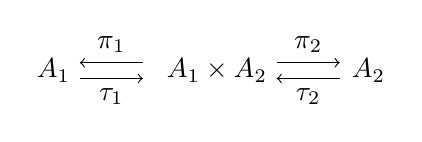
\begin{tikzpicture}
            \node [left] at (0,1) {$A_{1}$};
            \node [left] at (2.5,1) {$A_{1}\times A_{2}$};
            \node [left] at (4,1) {$A_{2}$};
            \draw [<-] (0,1.1)-- node [above, pos=0.5]{$\pi_{1}$} (0.8,1.1);
            \draw [->] (0,0.9)-- node [below, pos=0.5]{$\tau_{1}$} (0.8,0.9);
            \draw [->] (2.5,1.1)-- node [above, pos=0.5]{$\pi_{2}$} (3.3,1.1);
            \draw [<-] (2.5,0.9)-- node [below, pos=0.5]{$\tau_{2}$} (3.3,0.9);
        \end{tikzpicture}
    \end{figure}
    For any object $B$ such that

    \begin{figure}[H]\centering
        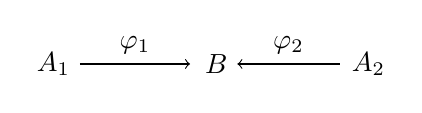
\begin{tikzpicture}
            \node [left] at (0,1) {$A_{1}$};
            \node [left] at (2,1) {$B$};
            \node [left] at (4,1) {$A_{2}$};
            \draw [->] (0,1)-- node [above, pos=0.5]{$\varphi_{1}$} (1.4,1);
            \draw [<-] (2,1)-- node [above, pos=0.5]{$\varphi_{2}$} (3.3,1);
        \end{tikzpicture}
    \end{figure}
    For any $(a_{1},a_{2})\in A_{1}\times A_{2}$, define $f:A_{1}\times A_{2}\to B$ as $f(a_{1},a_{2})=\varphi_{1}(a_{1})\varphi_{2}(a_{2})$. Then $f(\tau_{1}(a_{1}))=f(a_{1},e)=\varphi_{1}(a_{1})e=\varphi_{1}(a_{1})$, $f\circ \tau_{1}=\varphi_{1}$, $f(\tau_{2}(a_{2}))=f(e,a_{2})=e\varphi_{2}(a_{2})=\varphi_{2}(a_{2})$, $f\circ \tau_{2}=\varphi_{2}$.

    \begin{figure}[H]\centering
        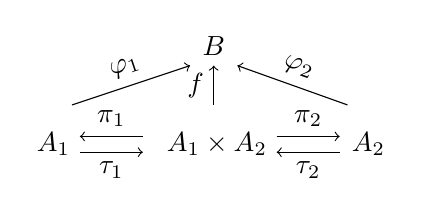
\begin{tikzpicture}
            \node [left] at (0,1) {$A_{1}$};
            \node [left] at (2.5,1) {$A_{1}\times A_{2}$};
            \node [left] at (4,1) {$A_{2}$};
            \draw [<-] (0,1.1)-- node [above, pos=0.5]{$\pi_{1}$} (0.8,1.1);
            \draw [->] (0,0.9)-- node [below, pos=0.5]{$\tau_{1}$} (0.8,0.9);
            \draw [->] (2.5,1.1)-- node [above, pos=0.5]{$\pi_{2}$} (3.3,1.1);
            \draw [<-] (2.5,0.9)-- node [below, pos=0.5]{$\tau_{2}$} (3.3,0.9);
            \node [above] at (1.7,2) {$B$};
            \draw [<-] (1.7,2)-- node [left, pos=0.5]{$f$} (1.7,1.5);
            \draw [<-] (1.4,2)-- node [above, pos=0.5, sloped]{$\varphi_{1}$} (-0.1,1.5);
            \draw [<-] (2,2)-- node [above, pos=0.5, sloped]{$\varphi_{2}$} (3.4,1.5);
        \end{tikzpicture}
    \end{figure}
    Next we verify the uniqueness. If there exist $f$ and $f'$ satisfies the condition, \[f(\tau_{1}(a_{1}))=f'(\tau_{1}(a_{1}))=f(a_{1},e)=f'(a_{1},e)\]\[f(\tau_{2}(a_{2}))=f'(\tau_{2}(a_{2}))=f(e,a_{2})=f'(e,a_{2})\]\[\begin{aligned}
        &f(\tau_{1}(a_{1}),\tau_{2}(a_{2}))=f(\tau_{1}(a_{1}))f(\tau_{2}(a_{2}))\\=&f'(\tau_{1}(a_{1}),\tau_{2}(a_{2}))=f'(\tau_{1}(a_{1}))f'(\tau_{2}(a_{2}))
    \end{aligned}\]
    so $f=f'$.
\end{answer}

$$ $$

\begin{ex}
    Every family $\{A_{i}|i\in I\}$ in the category of sets has a coproduct.
\end{ex}

\begin{answer}
    We examine $\bigcup\limits^{\cdot}A_{i}=\{(a,i)\in (\cup A_{i})\times I|a\in A_{i}\}$ which satisfies the condition. Define the morphism $\pi_{i}:A_{i}\to \bigcup\limits^{\cdot}A_{i}$ as $\pi_{i}(a)=(a,i)$. For any $B$ such that $\exists \varphi_{i}:A_{i}\to B$.
    
    \begin{figure}[H]\centering
        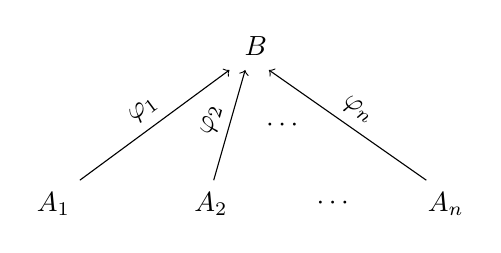
\begin{tikzpicture}
            \node [left] at (0,1) {$A_{1}$};
            \node [left] at (2,1) {$A_{2}$};
            \node [left] at (3.6,1) {$\cdots$};
            \node [left] at (5,1) {$A_{n}$};
            \node [left] at (2.5,3) {$B$};
            \draw [->] (0,1.3)-- node [above, pos=0.5, sloped]{$\varphi_{1}$} (1.9,2.7);
            \draw [->] (1.7,1.3)-- node [above, pos=0.5, sloped]{$\varphi_{2}$} (2.1,2.7);
            \draw [->] (4.4,1.3)-- node [above, pos=0.5, sloped]{$\varphi_{n}$} (2.4,2.7);
            \node [above] at (2.6,1.8) {$\cdots$};
        \end{tikzpicture}
    \end{figure}
    $\varphi(a)=x\in B$. Take $\varphi(a,i)=\varphi_{i}(a)$ defined on the subset of $\cup A_{i}\times I$, we can verify that the domain of $\varphi$ is $\bigcup\limits^{\cdot}A_{i}$. Then take $f=\varphi$, $f(\pi_{i}(a))=\varphi_{i}(a)$, $f\circ \pi_{i}=\varphi_{i}$.

    The uniqueness is obvious.
\end{answer}

$$ $$

\begin{ex}
    \begin{enumerate}[(a)]
        \item Show that in the category $\mathcal{S}_{*}$ of pointed sets product always exist; describe them.
        \item Show that in $\mathcal{S}_{*}$ every family of objects has a coproduct, describe the coproduct.
    \end{enumerate}
\end{ex}

\begin{answer}
    \begin{enumerate}[(a)]
        \item Define $\otimes$ as an operator between points and other elements in the pointed set. $\forall a\in A_{i}$, $a\otimes a_{i}=a_{1}\times a=a$. For a family of sets with their points $\{(A_{i},a_{i}|i\in I)\}$, consider $(A_{1}, A_{2}, \cdots, A_{n})=\{(a_{1}', a_{2}',\cdots, a_{n}')\}$. Define morphisms $\pi_{i}(a)=(a_{1}, a_{2},\cdots, a,\cdots, a_{n})$, $\pi_{i}:A_{i}\to (A_{1}, A_{2}, \cdots, A_{n})$.
        
        \begin{figure}[H]\centering
            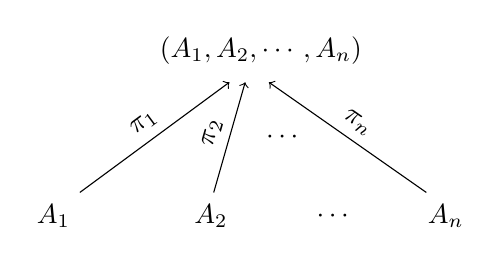
\begin{tikzpicture}
                \node [left] at (0,1) {$A_{1}$};
                \node [left] at (2,1) {$A_{2}$};
                \node [left] at (3.6,1) {$\cdots$};
                \node [left] at (5,1) {$A_{n}$};
                \node [above] at (2.3,2.8) {$(A_{1}, A_{2}, \cdots, A_{n})$};
                \draw [->] (0,1.3)-- node [above, pos=0.5, sloped]{$\pi_{1}$} (1.9,2.7);
                \draw [->] (1.7,1.3)-- node [above, pos=0.5, sloped]{$\pi_{2}$} (2.1,2.7);
                \draw [->] (4.4,1.3)-- node [above, pos=0.5, sloped]{$\pi_{n}$} (2.4,2.7);
                \node [above] at (2.6,1.8) {$\cdots$};
            \end{tikzpicture}
        \end{figure}
        For any $B$ such that $\exists \varphi_{i}:A_{i}\to B$.
    
        \begin{figure}[H]\centering
            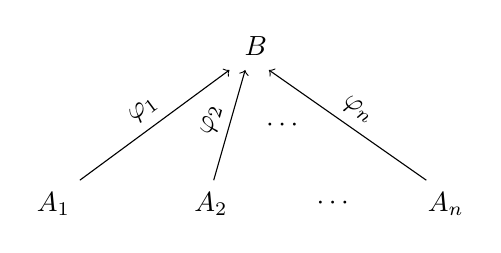
\begin{tikzpicture}
                \node [left] at (0,1) {$A_{1}$};
                \node [left] at (2,1) {$A_{2}$};
                \node [left] at (3.6,1) {$\cdots$};
                \node [left] at (5,1) {$A_{n}$};
                \node [left] at (2.5,3) {$B$};
                \draw [->] (0,1.3)-- node [above, pos=0.5, sloped]{$\varphi_{1}$} (1.9,2.7);
                \draw [->] (1.7,1.3)-- node [above, pos=0.5, sloped]{$\varphi_{2}$} (2.1,2.7);
                \draw [->] (4.4,1.3)-- node [above, pos=0.5, sloped]{$\varphi_{n}$} (2.4,2.7);
                \node [above] at (2.6,1.8) {$\cdots$};
            \end{tikzpicture}
        \end{figure}
        Take $f:(A_{1}, A_{2}, \cdots, A_{n})\to B$ as \[f(a_{1}',a_{2}',\cdots,a_{n}')=\varphi_{1}(a_{1}')\otimes\varphi_{2}(a_{2}')\otimes\cdots\otimes\varphi(a_{n}')\]Then $f\circ\pi_{i}(a)=f(a_{1},a_{2},\cdots,a,\cdots, a_{n})=\varphi_{1}(a_{1})\otimes\cdots\otimes\varphi_{i}(a)\otimes\cdots\otimes\varphi_{n}(a_{n})=\varphi_{i}(a)$. So $f\circ \pi_{i}=\varphi_{i}$.

        Next we verify the uniqueness. If there exist $f$ and $f'$ satisfies the condition. Then $\exists i\in I$ and $a\in A_{i}$ s.t. $f(a_{1},a_{2},\cdots,a,\cdots,a_{n})\neq f'(a_{1},a_{2},\cdots,a,\cdots,a_{n})$. But $f(\pi_{i}(a))=f'(\pi_{i}(a))$, so $f=f'$.
        \item The proof is similar to \textbf{Exercise 1.7.5}.
    \end{enumerate}
\end{answer}

$$ $$

\begin{ex}
    Let $F$ be a free object on a set $X(i:X\to F)$ in a concrete category $\mathcal{C}$. If $\mathcal{C}$ contains an object whose underlying set has at least two elements in it, then $i$ is an injective map of sets.
\end{ex}

\begin{answer}
    Assume $A\in\mathrm{obj}(\mathcal{C})$, $A$ has at least two elements and $X\xrightarrow{f} A$. $X\xrightarrow{i} F$ and $F$ is free on $X$, so there exists a morphism $\bar{f}$ s.t. $F\xrightarrow{\bar{f}}A$. If $\left| X \right|=1$, $i$ must be injective. For $\left| X \right| \geq 2$. Suppose $i$ is not injective. Take $x_{1}, x_{2}\in X$ and $i(x_{1})=i(x_{2})\in F$, $f(x_{1})=a_{1}$, $f(x_{2})=a_{2}$. $\bar{f}(i(x_{1}))=\bar{f}(i(x_{2}))=f(x_{1})=f(x_{2})=a_{1}=a_{2}$. That means all the elements in $A$ are identical. That's contradictory to the assumption.
\end{answer}

$$ $$

\begin{ex}
    Suppose $X$ is a set and $F$ is a free object on $X$ (with $i:X\to F$) in the category of groups. Prove that $i(X)$ is a set of generators for the group $F$.
\end{ex}

\begin{answer}
    Assume $G$ the subgroup of $F$ is the group generated by $i(X)$. Since $X\xrightarrow{i}G$ and $X\xrightarrow{i}F$, we can obtain unique morphism $\varphi$ such that $F\xrightarrow{\varphi}G$ and $\varphi \circ i=i$. 
    
    Consider morphism $1_{F}:F\to F$ which is the identical homomorphism. $F$ is free so $1_{F}$ is the unique homomorphism. Take $\subset:G\to F$ as a morphism defined as $\forall g\in G$, $\subset(g)=g$. Then
    
    \begin{figure}[H]\centering
        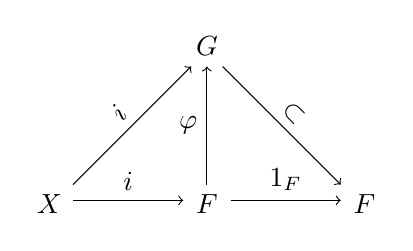
\begin{tikzpicture}
        \node [below] at (0,1) {$X$};
        \node [below] at (2,1) {$F$};
        \node [below] at (4,1) {$F$};
        \node [below] at (2,3) {$G$};
        \draw [->] (0.3,0.8)-- node [above, pos=0.5] {$i$} (1.7,0.8);
        \draw [->] (2.3,0.8)-- node [above, pos=0.5] {$1_{F}$} (3.7,0.8);
        \draw [->] (2,1)-- node [left, pos=0.5] {$\varphi$} (2,2.5);
        \draw [->] (0.3,1)-- node [above, pos=0.5, sloped] {$i$} (1.8,2.5);
        \draw [<-] (3.7,1)-- node [above, pos=0.5, sloped] {$\subset$} (2.2,2.5);
        \end{tikzpicture}
    \end{figure}
    $\subset\circ\varphi\circ i=1_{F}\circ i=i$ so $\subset\circ\varphi=1_{F}$. Thus $\subset$ is an epimorphism, $F\subset G$. So $F=G$ can be generated by $i(X)$.
\end{answer}
\section{Direct products and direct sums}
\begin{ex}
    $S_{3}$ is not the direct product of any family of its proper subgroups. The same is true of $Z_{p^{n}}$($p$ prime, $n\geq 1$) and $\mathbb{Z}$.
\end{ex}

$$ $$

\begin{ex}
    Give an example of groups $H_{i}$, $K_{i}$ such that $H_{1}\times H_{2}\cong K_{1}\times K_{2}$ and no $H_{i}$ is isomorphic to any $K_{j}$.
\end{ex}

$$ $$

\begin{ex}
    Let $G$ be and (additive) abelian group with subgroups $H$ and $K$. Show that $G\cong H\oplus K$ if and only if there are homomorphisms 
    
    \begin{figure}[H]\centering
        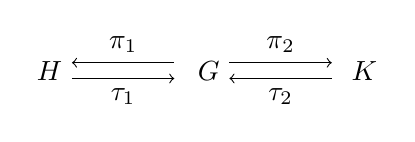
\begin{tikzpicture}
            \node [left] at (0,1) {$H$};
            \node [left] at (2,1) {$G$};
            \node [left] at (4,1) {$K$};
            \draw [<-] (0,1.1)-- node [above, pos=0.5]{$\pi_{1}$} (1.3,1.1);
            \draw [->] (0,0.9)-- node [below, pos=0.5]{$\tau_{1}$} (1.3,0.9);
            \draw [->] (2,1.1)-- node [above, pos=0.5]{$\pi_{2}$} (3.3,1.1);
            \draw [<-] (2,0.9)-- node [below, pos=0.5]{$\tau_{2}$} (3.3,0.9);
        \end{tikzpicture}
    \end{figure}
    such that $\pi_{1}\tau_{1}=1_{H}$, $\pi_{2}\tau_{2}=1_{K}$, $\pi_{1}\tau_{2}=0$ and $\pi_{2}\tau_{1}=0$, where 0 is the map sending every element onto the zero (identity) element, and $\tau_{1}\pi_{1}(x)+\tau_{2}\pi_{2}(x)=x$ for all $x\in G$.
\end{ex}

$$ $$

\begin{ex}
    Give an example to show that the weak direct product is not a coproduct in the category of all groups.
\end{ex}

$$ $$

\begin{ex}
    Let $G$, $H$ be finite cyclic groups. Then $G\times H$ is cyclic if and only if $(\left| G \right|, \left| H \right|  )=1$.
\end{ex}

$$ $$

\begin{ex}
    Every finitely generated abelian group $G\neq\left\langle e\right\rangle$ in which every element (except $e$) has order $p$ ($p$ prime) is isomorphic to $Z_{p}\oplus Z_{p}\oplus\cdots\oplus Z_{p}$($n$ summands) for some $n\geq 1$.
\end{ex}

$$ $$

\begin{ex}
    Let $H,K,N$ be nontrivial normal subgroups of a group $G$ and suppose $G=H\times K$. Prove that $N$ is in the center of $G$ or $N$ intersects one of $H,K$ nontrivially. Give examples to show that both possibilities can actually occur when $G$ is nonabelian.
\end{ex}

$$ $$

\begin{ex}
    Corollary 8.7 is false if one of the $N_{i}$ is not normal.
\end{ex}

$$ $$

\begin{ex}
    If a group $G$ is the (internal) direct product of its subgroups $H$, $K$, then $H\cong G / K$ and $G /H \cong K$.
\end{ex}

$$ $$

\begin{ex}
    If $\{G_{i}|i\in I\}$ is a family of groups, then $\prod^{w}G_{i}$ is the internal weak product its subgroups $\{\tau_{i}(G_{i})|i\in I\}$.
\end{ex}

$$ $$

\begin{ex}
    Let $\{N_{i}|i\in I\}$ be a family of subgroups of a group $G$. Then $G$ is the internal weak product of $\{N_{i}|i\in I\}$if and only if:
    \begin{enumerate}[(i)]
        \item $a_{i}a_{j}=a_{j}a_{i}$ for all $i\neq j$ and $a_{i}\in N_{i}$, $a_{j}\in N_{j}$;
        \item every nonidentity element of $G$ is uniquely a product $a_{i_{1}}\cdots a_{i_{n}}$, where $i_{i},\dots,i_{n}$ are distinct elements of $I$ and $e\neq a_{i_{k}}\in N_{i_{k}}$ for each $k$.
    \end{enumerate}
\end{ex}

$$ $$

\begin{ex}
    A normal subgroup $H$ of a group $G$ is said to be a \textbf{direct factor} (\textbf{direct summand} if $G$ is additive abelian) if there exists a (normal) subgroup $K$ of $G$ such that $G=H\times K$.
    \begin{enumerate}[(a)]
        \item If $H$ is a direct factor of $K$ and $K$ is a direct factor of $G$, then $H$ is normal in $G$.
        \item If $H$ is a direct factor of $G$, then every homomorphism $H\to G$ may be extended to an endomorphism $G\to G$. However, a monomorphism $H\to G$ need not be extendible to and automorphism $G\to G$.
    \end{enumerate}
\end{ex}

$$ $$

\begin{ex}
    Let $\{G_{i}|i\in I\}$ be a family of groups and $J\subset I$. The map $\alpha: \prod\limits_{j\in J}G_{j}\to \prod\limits_{i\in I}G_{i}$ given by $\{a_{j}\}\mapsto \{b_{i}\}$, where $b_{j}=a_{j}$ for $j\in J$ and $b_{i}=e_{i}$(identity in $G_{i}$) for $i\notin J$, is a monomorphism of groups and $\prod\limits_{i\in I}G_{i} /\alpha(\prod\limits_{j\in J}G_{j})\cong \prod\limits_{i\in I-J}G_{i}$.
\end{ex}

$$ $$

\begin{ex}
    For $i=1,2$ let $H_{i}\lhd G_{i}$ and give examples to show that each of the following statements may be false:
    \begin{enumerate}[(a)]
        \item $G_{1}\cong G_{2}$ and $H_{1}\cong H_{2}\Rightarrow G_{1} /H_{1}\cong G_{2} /H_{2}$.
        \item $G_{1}\cong G_{2}$ and $G_{1}/ H_{1}\cong G_{2} / H_{2}\Rightarrow H_{1}\cong H_{2}$.
        \item $H_{1}\cong H_{2}$ and $G_{1}/ H_{1}\cong G_{2} / H_{2}\Rightarrow G_{1}\cong G_{2}$.
    \end{enumerate}
\end{ex}
\section{Free groups, free products, generators and relations}
\begin{ex}
    Every nonidentity elements in a free group $F$ has a infinite order.
\end{ex}

\begin{answer}
    Define the length of a word $x=a_{1}^{\lambda_{1}}a_{2}^{\lambda_{2}}\cdots a_{n}^{\lambda_{n}}$ is $n$ and denote it as $len(x)$. Assume $len(x)=n$ for some $n\in F$ and $len(1)=0$, we prove that $len(x^{m})\geq n\forall m\geq 1$.

    Let $k$ be the largest integer such that  $a_{n-j}^{\lambda_{n-j}}=a_{n}^{-\lambda_{j}}$ for $j=0, 1, \dots, k-1$. If $k>\left[\frac{n}{2}\right]$. For even $k$, $a_{\frac{n}{2}}^{\lambda_{\frac{n}{2}}}=a_{\frac{n}{2}+1}^{-(\lambda_{\frac{n}{2}+1})}$, $a_{\frac{n}{2}-1}^{\lambda_{\frac{n}{2}-1}}=a_{\frac{n}{2}+2}^{-(\lambda_{\frac{n}{2}+2})}$, $\cdots$ which means $x=a_{1}^{\lambda_{1}}a_{2}^{\lambda_{2}}\cdots a_{n}^{\lambda_{n}}=1$. For odd $k$, $a_{\left[\frac{n}{2}\right]+1}^{\lambda_{\left[\frac{n}{2}\right]+1}}=a_{\left[\frac{n}{2}\right]+1}^{-(\lambda_{\left[\frac{n}{2}\right]+1})}$, which is contradictory to $x$ is reduced. So $k\leq \left[\frac{n}{2}\right]$.

    Divide $x=x_{1}x_{2}x_{3}$ where $x_{1}=a_{1}^{\lambda_{1}}\cdots a_{k}^{\lambda_{k}}$, $x_{2}=a_{k+1}^{\lambda_{k+1}}\cdots a_{n-k}^{\lambda_{n-k}}$, $x_{3}=a_{n-k+1}^{\lambda_{n-k+1}}\cdots a_{n}^{\lambda_{n}}$. $x_{3}x_{1}=1$. So $len(x)=len(x_{1})+len(x_{2})+len(x_{3})=n$. $x^{m}=x_{1}x_{2}x_{3}x_{1}x_{2}x_{3}\cdots x_{1}x_{2}x_{3}=x_{1}x_{2}^{m}x_{3}$. $len(x^{m})=len(x_{1})+m\cdot len(x_{2})+len(x_{3})\geq n$. So $\forall m\geq 1$, $x^{m}\neq 1$, $\left| x \right| $ is infinite.
\end{answer}

$$ $$

\begin{ex}
    Show that the free group on the set $\{a\}$ is an infinite cyclic group, and hence isomorphic to $\mathbf{Z}$.
\end{ex}

\begin{answer}
    $F(\{a\})=\left\langle a\right\rangle$ and thus it's a infinite cyclic group. $F(\{a\})\cong \mathbf{Z}$.
\end{answer}

$$ $$

\begin{ex}
    Let $F$ be a free group and let $N$ be the subgroup generated by the set $\{x^{n}|x\in F, n\text{ a fixed integer}\}$. Show that $N\lhd F$.
\end{ex}

$$ $$

\begin{ex}
    Let $F$ be the free group on the set $X$, and let $Y\subset H$. If $H$ is the smallest normal subgroup of $F$ containin $Y$, then $F /H$ is a free group.
\end{ex}

$$ $$

\begin{ex}
    The group defined by generators $a,b$ and relations $a^{8}=b^{2}a^{4}=ab^{-1}ab=e$ has order at most 16.
\end{ex}

$$ $$

\begin{ex}
    The cyclic group of order 6 is the group defined by generators $a, b$ and relations $a^{2}=b^{3}=a^{-1}b^{-1}ab=e$.
\end{ex}

$$ $$

\begin{ex}
    Show that the group defined by generators $a, b$ and relations $a^{2}=e$, $b^{3}=e$ is infinite and nonabelian.
\end{ex}

$$ $$

\begin{ex}
    The group defined by generators $a, b$ and relations $a^{n}=e (3\leq n\in \mathbf{N}^{*})$, $b^{2}=e$ and $abab=e$ is the dihedral group $D_{n}$.
\end{ex}

$$ $$

\begin{ex}
    The group defined by the generator $b$ and $b^{m}=e(m\in \mathbf{N}^{*})$ is the cyclic group $Z_{m}$.
\end{ex}

$$ $$

\begin{ex}
    The operation of free product is commutative and associative: for any groups $A$, $B$, $C$, $A*B\cong B*A$ and $A*(B*C)\cong (A*B)*C$.
\end{ex}

$$ $$

\begin{ex}
    If $N$ is normal subgroup of $A*B$ generated by $A$, then $(A*B) /N\cong B$.
\end{ex}

$$ $$

\begin{ex}
    If $G$ and $H$ each have more than one element, then $G*H$ is an infinite group with center $\left\langle e\right\rangle$.
\end{ex}

$$ $$

\begin{ex}
    A free group is a free product of infinite cyclic groups.
\end{ex}

$$ $$

\begin{ex}
    If $G$ is the group defined by generators $a, b$ and relations $a^{2}=e$, $b^{3}=e$, then $G\cong Z_{2}*Z_{3}$.
\end{ex}

$$ $$

\begin{ex}
    If $f:G_{1}\to G_{2}$ and $g:H_{1}\to H_{2}$ are homomorphisms of groups, then there is a unique homomorphism $h:G_{1}*H_{1}\to G_{2}H_{2}$ such that $h|G_{1}=f$ and $h|H_{1}=g$.
\end{ex}

\chapter{The structure of groups}

\chapter{Rings}
\section{Sequence and their Limits}
\begin{definition}
    We call $A$ is the \textbf{limit} of a sequence, if for any neighborhood $V(A)$ around $A$, there exists a serial number $N$ (related to $V(A)$), any item has serial number larger than which will be contained in $V(A)$.
\end{definition}
Now we give the rigorous definition of limit of a sequence:\

\begin{definition}
    $A\in R$ is a limit of a sequence, if for any $\varepsilon >0$, there exists a number $N$, for all $n>N$, $\left\lvert x_{n}-A\right\lvert<\varepsilon$.    
\end{definition}

Denotion $\lim\limits_{n \to \infty}x_{n}\to A$ are used to indicate the limit of $\{x_{n}\}$.
\[\left(\lim\limits_{n \to \infty}x_{n}=A\right):=\forall V(A)\ \exists N\in \mathbb{N}\ \forall n>N\ (x_{n}\in V(A)) \]
or
\[\left(\lim\limits_{n \to \infty}x_{n}=A\right):=\forall \varepsilon>0\ \exists N\in \mathbb{N}\ \forall n>\mathbb{N}\ (\left| x_{n}-A \right|<\varepsilon )\]

\begin{definition}
    If $\lim\limits_{n \to \infty}x_{n}=A$, we say that $\{x_{n}\}$ converges to or tend to $A$. We call it the convergent sequences. The sequences doesn't have a limit is named divergent sequence.
\end{definition}
\section{Ideals}
\begin{ex}
    The set of all nilpotent elements in a commutative ring forms an ideal.
\end{ex}

\begin{answer}
    Assume the set is $I$, then $\forall a,b\in I$, $a^{m}=b^{n}=0$, $(a+b)^{m+n}=0$ and $(ab)^{mn}=0$ so $a+b\in I$, $ab\in I$. $I$ is a subring. $\forall x\in R$, $(xa)^{m}=x^{m}a^{m}=0$, $(ax)^{m}=a^{m}x^{m}=0$, so $xa\in I$ and $ax\in I$, $I$ is an ideal.
\end{answer}

$$ $$

\begin{ex}
    Let $I$ be an ideal in a commutative ring $R$ and let $\mathrm{Rad} I=\{r\in R| r^{n}\in I \text{ for some } n\}$. Show that $\mathrm{Rad}I$ is an ideal.
\end{ex}

\begin{answer}
    $\mathrm{Rad} I$ is a ring since $R$ is a commutative ring. For $r\in \mathrm{Rad} I$ and $\forall x\in R$, $(xr)^{n}=x^{n}r^{n}\in I$ so $xr\in \mathrm{Rad} I$, $(rx)^{n}=r^{n}x^{n}\in I$ so $rx\in \mathrm{Rad} I$. Thus $\mathrm{Rad} I$ is an ideal.
\end{answer}

$$ $$

\begin{ex}
    If $R$ is a ring and $a\in R$, then $J=\{r\in R|ra=0\}$ is a left ideal and $K=\{r\in R|ar=0\}$ is a right ideal in $R$.
\end{ex}

\begin{answer}
    $J$ is a subring of $R$. For $r\in J$ and $\forall x\in R$, $(xr)a=x(ra)=0$ so $xr\in J$, $J$ is a left ideal. Similarly, $I$ is a right ideal.
\end{answer}

$$ $$

\begin{ex}
    If $I$ is a left ideal of $R$, then $A(I)=\{r\in R|rx=0 \text{ for every }x\in I\}$ is an ideal in $R$.
\end{ex}

\begin{answer}
    For any $a,b\in A(I)$, we have $ab\in A(I)$ and $a+b\in A(I)$. For $r\in A(I)$ and $\forall x\in R$, $(xr)x'=x(rx')=0$ for every $x'\in I$, so $xr\in A(I)$. $(rx)x'=r(xx')$, $x x'\in I$ so $rx x'=0$, $rx\in A(I)$. Thus $A(I)$ is an ideal of $R$.
\end{answer}

$$ $$

\begin{ex}
    If $I$ is an ideal in a ring $R$, let $\left[R:I\right]=\{r\in R|xr\in I \text{ for every }x\in R\}$. Prove that $\left[ R:I\right]$ is an ideal of $R$ which contains $I$.
\end{ex}

\begin{answer}
    $I$ is a subring of $R$ so $\left[R:I\right]$ is also a subring of $R$. For $r\in\left[R:I\right]$ and $x, x'\in R$, $x'xr=(x'x)r\in I$ so $xr\in \left[R:I\right]$, $x'rx=(x'r)x\in I$ so $rx\in \left[R:I\right]$. $\left[R:I\right]$ is an ideal of $R$. Since $\forall r\in I$, $xr\in I$ and $rx\in I$, $I\subset \left[R:I\right]$.
\end{answer}

$$ $$

\begin{ex}
    \begin{enumerate}[(a)]
        \item The center of the ring $S$ of all $2\times 2$ matrices over a field $F$ consists of all matrices of the form $\begin{pmatrix}
            a&0\\0&a
        \end{pmatrix}$.
        \item Then center of $S$ is not an ideal in $S$.
        \item What is the center of the ring of all $n\times n$ matrices over a division ring?
    \end{enumerate}
\end{ex}

\begin{answer}
    \begin{enumerate}[(a)]
        \item $\forall x\in M_{F}(2,2)$, $x=\begin{pmatrix}
            x_{1}&x_{2}\\x_{3}&x_{4}
        \end{pmatrix}$\[x\begin{pmatrix}
            a&0\\0&a
        \end{pmatrix}=\begin{pmatrix}
            a&0\\0&a
        \end{pmatrix}x=\begin{pmatrix}
            ax_{1}&ax_{2}\\ax_{3}&ax_{4}
        \end{pmatrix}\] so $\begin{pmatrix}
            a&0\\0&a
        \end{pmatrix}\in C(M_{F}(2,2))$.

        $\forall \begin{pmatrix}
            a_{1}&a_{2}\\a_{3}&a_{4}
        \end{pmatrix}\in C(M_{F}(2,2))$, take $\begin{pmatrix}
            0&1_{F}\\0&0
        \end{pmatrix}\in M_{F}(2,2)$\[\begin{pmatrix}
            a_{1}&a_{2}\\a_{3}&a_{4}
        \end{pmatrix}\begin{pmatrix}
            1_{F}&0\\0&0
        \end{pmatrix}=\begin{pmatrix}
            a_{1}&0\\a_{3}&0
        \end{pmatrix}\]\[\begin{pmatrix}
            1_{F}&0\\0&0
        \end{pmatrix}\begin{pmatrix}
            a_{1}&a_{2}\\a_{3}&a_{4}
        \end{pmatrix}=\begin{pmatrix}
            a_{1}&a_{2}\\0&0
        \end{pmatrix}\] so $a_{2}=a_{3}=0$.
        \[\begin{pmatrix}
            a_{1}&a_{2}\\a_{3}&a_{4}
        \end{pmatrix}\begin{pmatrix}
            0&1_{F}\\0&0
        \end{pmatrix}=\begin{pmatrix}
            0&a_{1}\\0&a_{3}
        \end{pmatrix}\]\[\begin{pmatrix}
            0&1_{F}\\0&0
        \end{pmatrix}\begin{pmatrix}
            a_{1}&a_{2}\\a_{3}&a_{4}
        \end{pmatrix}\begin{pmatrix}
            a_{3}&a_{4}\\0&0
        \end{pmatrix}\] so $a_{1}=a_{4}$. All the elements of $C(M_{F}(2,2))$ has the form $\begin{pmatrix}
            a&0\\0&a
        \end{pmatrix}$.
        \item For $c\in C(S)$. If $S$ is not commutative, $\forall x,x'\in R$, we need $xc\in C(S)\Rightarrow x'xc=xcx'=xx'c$, however, this may not always true.
        \item By multiplying $\begin{pmatrix}
            1_{F}& &\\ &\ddots & \\ & &0
        \end{pmatrix}$, $\begin{pmatrix}
            0& & &\\ &1_{F}& &\\ & &\ddots&\\ & & &0
        \end{pmatrix}$, $\dots$, $\begin{pmatrix}
            0& &\\ &\ddots & \\ & &1_{F}
        \end{pmatrix}$, we can have $C(M_{F}(2,2))$ consist of all the elements in the form of $a\begin{pmatrix}
            1_{F}& & &\\ &1_{F}& &\\ & &\ddots&\\ & & &1_{F}
        \end{pmatrix}$.
    \end{enumerate}
\end{answer}
$$ $$

\begin{ex}
    \begin{enumerate}[(a)]
        \item A ring $R$ with identity is a division ring if and only if $R$ has no proper left ideals.
        \item If $S$ is a ring (possibly without identity) with no proper left ideals, then either $S^{2}=0$ or $S$ is a division ring.
    \end{enumerate}
\end{ex}

\begin{answer}
    \begin{enumerate}[(a)]
        \item Suppose not. $I$ is an ideal in $R$. $\forall r\in I$, take $r^{-1}\in R$, then $1_{R}\in I$ so $I=R$ is not a  proper ideal.
        \item $I=\{a\in S|Sa=0\}$ is a left ideal since $\forall x,x'\in S$, $x'(xs)=(x'x)s=0$, $xs\in I$. Thus $I=0$ or $I=S$. If $I=S$, then $S^{2}=0$. If $I=0$, we prove $S$ has no zero divisor.
        
        For the set $I'=\{r\in S|rb=0\}$, $I'\subset I$. $I'$ is a subring of $S$, and $I'$ is also a left ideal of $S$. So $I'=0$, $b$ has no left zero divisors. $\forall a\in S$, $Sa$ is a left ideal of $S$. $Sa\neq 0$ so $Sa=S$. Thus, $\exists 1_{S}\in S$, such that $1_{S}a=a$. Since $s_{1}-s_{2}$ has no left zero divisor, $as_{1}=as_{2}\Rightarrow s_{1}=s_{2}$. So $aS=S$. For all $s\in S$, $\exists s'$ s.t. $s=as'$ so $\forall s\in S$, $1_{S}\cdot s=1_{S}as'=as'=s$. $aS=S$ so $\exists 1_{S}'\in S$, $a1_{S}'=a$. Similarly, $\forall s\in S$, $s1_{S}=s$. Then $1_{S}1_{S}'=1_{S}=1_{S}'$ so $S$ has identity. Since $Sa=aS=S$, we can have $S$ is a division ring.
    \end{enumerate}
\end{answer}

$$ $$

\begin{ex}
    Let $R$ be a ring with identity and $S$ the ring of all $n\times n$ matrices over $R$. $J$ is an ideals of $S$ if and only if $J$ is the ring of all $n\times n$ matrices over $I$ for some ideal $I$ in $R$.
\end{ex}

\begin{answer}
    If $J$ is an ideal. Denote $E_{r,s}$ as the matrix which has $1_{R}$ as the $r$ column and $s$ row. Then $\forall A=(a_{ij})$, $E_{p,r}AE_{s,q}$ is a matrix with $a_{rs}$ in the $p$ column and  $q$ row. So for $A\in J$ $(aE_{p,r})A(bE_{s,q})$ is the matrix with $aa_{rs}b$ in the $p$ column and  $q$ row. $aa_{rs}b\in I$. Then because of closure we know $J$ contains all $n\times n$ matrices over $I$. 

    If $J$ consists of all $n\times n$ matrices over $I$, the proof is trivial.
\end{answer}

$$ $$

\begin{ex}
    Let $S$ be the ring of all $n\times n$ matrices over a division ring $D$.
    \begin{enumerate}[(a)]
        \item $S$ has no proper ideals (that is, 0 is the maximal ideal).
        \item $S$ has zero divisors. Consequently, (i) $S\cong S /0$ is not a division ring and (ii) 0 is a prime ideal which does not satisfy condition (1) of Theorem 2.15.
    \end{enumerate}
\end{ex}

\begin{answer}
    \begin{enumerate}[(a)]
        \item $J$ is an ideal of $S$ so $J$ consists of all $n\times n$ matrices over $I$ where $I$ is an ideal of $D$. From \textbf{Exercise 3.2.7}, $D$ has no proper ideal so $I=0\Rightarrow J=0$.
        \item For $A=(a_{ij})$ with $a_{ri}=0$ for $i=1,2\cdots$ and other entries doesn't equals to zero, we have $E_{1r}A=0$. $S$ has no zero divisors.
    \end{enumerate}
\end{answer}

$$ $$

\begin{ex}
    \begin{enumerate}[(a)]
        \item Show that $\mathbf{Z}$ is a principle ideal ring.
        \item Every homomorphic image of a principle ideal ring is also a principle ideal ring.
        \item $Z_{m}$ is a principle ideal ring for every $m>0$.
    \end{enumerate}
\end{ex}

\begin{answer}
    \begin{enumerate}[(a)]
        \item For any ideal $I$ in $\mathbf{Z}$, $I$ is a subring so $I=m\mathbf{Z}$ where $m\in \mathbf{Z}$. $m\mathbf{Z}=(m)$ is a principle ideal so $\mathbf{Z}$ is a PID.
        \item For $f:R\to S$ with $f(r)=s$ and $R$ is a principle ideal ring. Consider $f:R\to \mathrm{Im}f\subset S$. For any ideal $J\subset \mathrm{Im}f$, $f^{-1}(J)$ is an ideal since $\forall a\in f^{-1}(J)$ and $r\in R$, $f(ar)=f(a)f(r)\in J\Rightarrow ar\in f^{-1}(J)$. $f^{-1}(J)$ is a principle ideal, assume $f^{-1}(J)=(a)$. Then $\forall r\in R$, $ar\in (a)$, $ra\in (a)$. $f(ar)=f(a)f(r)\in J$ and $f(ra)=f(r)f(a)\in J$ since $f(a)\in J$ and $f(r)\in S$. So $(f(a))\subset J$. $J=f((a))=\{f(ra+as+na+\sum\limits_{i=1}^{m}r_{i}as_{i})| r, s, r_{i}, s_{i}\in R, n\in \mathbf{Z}\}=\{f(r)f(a)+f(a)f(s)+nf(a)+\sum\limits_{i=1}^{m}f(r_{i})f(a_{i})f(s_{i})| r, s, r_{i}, s_{i}\in R, n\in \mathbf{Z}\}\subset (f(a))$. So $J=(f(a))$ is a principle ideal. The image of a principle ideal ring is also a principle ideal ring.
    \end{enumerate}
\end{answer}

$$ $$

\begin{ex}
    If $N$ is the ideal of all nilpotent elements in a commutative ring $R$, then $R /N$ is a ring with no nonzero nilpotent elements.
\end{ex}

\begin{answer}
    Suppose not. $\exists r\in R$, $r\notin N$, $(r+N)^{n}=0$ for some $n\in\mathbf{N}$. \[(r+N)^{n}=r^{n}+N=N\Rightarrow r^{n}\in N\]so for some $m\in \mathbf{N}$, $r^{nm}=0\Rightarrow r\in N$. That's contradictory!
\end{answer}

$$ $$

\begin{ex}
    Let $R$ be a ring without identity and with no zero divisors. Let $S$ be the ring whose additive group is $R\times \mathbf{Z}$ as in the proof of Theorem 1.10. Let $A=\{(r,n)\in S|rx+nx=0 \text{ for every }x\in R\}$.
    \begin{enumerate}[(a)]
        \item $A$ is an ideal in $S$.
        \item $S /A$ has an identity and contains a subring isomorphic to $R$.
        \item $S /A$ has no zero divisors.
    \end{enumerate}
\end{ex}

\begin{answer}
    \begin{enumerate}[(a)]
        \item For $(r,n), (r',n')\in S$, $(r'+r)x+(n'+j)x=rx+nx+r'x+n'x=0$, so $(r+r',n+n')\in A$. $(r,n)(r'n')=(rr'+nr'+n'r,nn')$, $rr'x+n'rx+nr'x+nn'x=r(r'x+n'x)+n(r'x+n'x)=0$, so $(r,n)(r',n')\in A$. $A$ is a subring of $R\times \mathbf{Z}$. $\forall (r_{1},n_{1})\in R\times \mathbf{Z}$, $(r_{1},n_{1})(r,n)=(r_{1}r+nr_{1}+n_{1}r,nn_{1})\Rightarrow r_{1}rx+nr_{1}x+n_{1}rx+nn_{1}x=r_{1}(rx+nx)+n_{1}(rx+nx)=0\Rightarrow (r_{1},n_{1})(r,n)\in A$. $A$ is an ideal of $R\times \mathbf{Z}$.
        \item Take $0_{R}\in R$ and $(0_{R},1)\in S$. Then $(0_{R},1)+A$ is an identity of $S /A$. \[\forall (r,n)\in S, \quad (r,n)(0_{R},1)=(0_{R},1)(r,n)=(r,n)\]
        \item For any $(r,n), (s,m)$ satisfy that $(r,n)(s,m)\in A$, we prove that $(r,n)\in A$ or $(s,m)\in A$. Suppose $sx+mx\neq 0$, $r(sx+mx)+n(sx+mx)=0\Rightarrow (sx+mx)r(sx+mx)+n(sx+mx)^{2}=0\Rightarrow ((sx+mx)r+n(sx+mx))(sx+mx)=0\Rightarrow (sx+mx)r+n(sx+mx)=0$. For any $x\in R$, $(sx+mx)rx+n(sx+mx)x=0\Rightarrow(sx+mx)(rx+nx)=0\Rightarrow rx+nx=0$, so $(r,n)\in A$. $S /A$ has no divisor.
    \end{enumerate}
\end{answer}

$$ $$

\begin{ex}
    Let $f:R\to S$ be a homomorphism of rings, $I$ and ideal in $R$, and $J$ an ideal in $S$.
    \begin{enumerate}[(a)]
        \item $f^{-1}(J)$ is and ideal in $R$ that contains $\mathrm{Ker}f$.
        \item If $f$ is an epimorphism, then $f(I)$ is an ideal in $S$. If $f$ is not surjective, $f(I)$ need not be an ideal.
    \end{enumerate}
\end{ex}

\begin{answer}
    \begin{enumerate}[(a)]
        \item $\forall a\in f^{-1}(J)$ and $r\in R$, $f(ar)=f(a)f(r)\in J\Rightarrow ar\in J$. Similarly, $ra\in J$, $f^{-1}(J)$ is an ideal. $\mathrm{Ker}f\subset f^{-1}(J)$ since $0_{S}\in J$.
        \item $\forall b\in f(I)$ and $s\in S$, $f$ is a epimorphism so $s=f(r)$, $b=f(a)$ for some $r, a\in R$. $sb=f(r)f(a)=f(ar)$, $ar\in I\Rightarrow sb\in f(I)$, similarly $bs\in f(I)$. $f(I)$ is an ideal.
        
        If $f$ is not surjective. Take $Z\left[x\right]$ and $\mathbf{Z}$ which is a subring but not an ideal in $Z\left[x\right]$. $\mathbf{Z}$ is an ideal of itself, $f=1_{\mathbf{Z}}$ satisfies the condition.
    \end{enumerate}
\end{answer}

$$ $$

\begin{ex}
    If $P$ is an ideal in a not necessarily commutative ring $R$, then the following conditions are equivalent.
    \begin{enumerate}[(a)]
        \item $P$ is a prime ideal.
        \item If $r,s\in R$ are such that $rRs\subset R$, then $r\in P$ or $s\in P$.
        \item If $(r)$ and $(s)$ are principle ideals of $R$ such that $(r)(s)\subset P$, then $r\in P$ or $s\in P$.
        \item If $U$ and $V$ are right ideals in $R$ such that $UV\subset R$, then $U\subset R$ or $V\subset R$.
        \item If $U$ and $V$ are left ideals in $R$ such that $UV\subset R$, then $U\subset R$ or $V\subset R$.
    \end{enumerate}
\end{ex}

$$ $$

\begin{ex}
    The set consisting of zero and all zero divisors in a commutative ring with identity contains at least one prime ideal.
\end{ex}

\begin{answer}
    Denote $S=R-Z$. $\forall a,b\in S$, we prove that $ab\in S$. Suppose $\exists (ab)c=0$ for some $c\in R$, $a$, $b$ are not zero divisors so $abc=b(ac)=a(bc)=0$, so $ac=0$, $bc=0\Rightarrow c=0$, so $ab$ is not a zero divisor. Thus $Z=R-S$ contains an prime ideal.
\end{answer}

$$ $$

\begin{ex}
    Let $R$ be a commutative ring with identity and suppose that the ideal $A$ of $R$ is contained in a finite union of prime ideals $P_{1}\cup\cdots\cup P_{n}$. Show that $A\subset P_{i}$ for some $i$.
\end{ex}

\begin{answer}
    Suppose not. We choose the smallest $I$ such that for all $i\in I$, $P_{i}\cap A\neq \varnothing$ and $A\cap P_{i}\not\subset\bigcup\limits_{j\neq i}P_{j}$ for any $i\in I$. So $\exists a_{i}\in (A\cap P_{i})-(\bigcup\limits_{j\neq i}P_{j})$, $\forall i\in I$. Take $x=a_{1}+a_{2}a_{3}\cdots a_{n}$, $x\in A$ since $a_{i}\in A$ for all $i\in I$. And $x\notin P_{i}$ for $i=2,3,\dots, n$ since $a_{1}\notin P_{i}$, $i=2,3,\dots, n$. $x\notin P_{1}$ since $P_{1}$ is prime and $a_{2}, \dots, a_{n}\notin P_{1}$. So $x\notin \bigcup\limits_{j\neq i}P_{j}$, which is contradictory!
\end{answer}

$$ $$

\begin{ex}
    Let $f:R\to S$ be an epimorphism of rings with kernel $K$.
    \begin{enumerate}[(a)]
        \item If $P$ is a prime ideal in $R$ that contains $K$, then $f(P)$ is a prime ideal in $S$.
        \item If $Q$ is a prime ideal in $S$, then $f^{-1}(Q)$ is a prime ideal in $R$ that contains $K$.
        \item There is a one-to-one correspondence between the set of all prime ideals in $R$ that contain $K$ and the set of all prime ideals in $S$, given by $P\mapsto f(P)$.
        \item If $I$ is an ideal in a ring $R$, then every prime ideal in $R /I$ is of the form $P /I$, where $P$ is a prime ideal in $R$ that contains $I$.
    \end{enumerate}
\end{ex}

\begin{answer}
    \begin{enumerate}[(a)]
        \item From \textbf{Exercise 3.2.13} we know $f(P)$ is an ideal. $\forall x,y\in f(P)$, $\exists a.b\in R$, $x=f(a)$, $y=f(b)$ and $a,b\notin P$. Assume $\exists p\in P$ such that $f(ab)=f(p)$, then $f(ab-p)=0$, $ab-p\in\mathrm{Ker}f\subset P\Rightarrow ab\in P$. That's contradictory to $a,b\notin P$ so $xy\notin f(P)$. $f(P)$ is prime.
        \item From \textbf{Exercise 3.2.13}, $f^{-1}(Q)$ is an ideal. Take $g:S\to S /Q$ and $gf:R\to S /Q$. By the Theorem of homomorphism, $R /f^{-1}(Q) \cong S /Q$ is a ring without divisor, so $f^{-1}(Q)$ is prime.
        \item From (a), (b), $f$ is a one-to-one map between prime ideals given by $P\mapsto f(P)$.
        \item Consider the homomorphism $f:R\to R /I$. For any prime ideal $P\subset R$ and $f(P)$ is an prime ideal in $R$, $\mathrm{Ker}f=I$ so for prime ideals $I\subset P\subset R$. $P$ can have one to one correspondence with $f(P)=P /I\subset R/I$. So all the prime ideals has the form $P /I$.
    \end{enumerate}
\end{answer}

$$ $$

\begin{ex}
    An ideal $M\neq R$ in a commutative ring $R$ with identity is maximal if and only if for every $r\in R-M$, there exists $x\in R$ such that $1_{R}-rx\in M$.
\end{ex}

\begin{answer}
    If $M$ is maximal, then $M$ is prime. So $rR+M=R$, $r(R-M)+M=R$ and $r(R-M)\cap M=\varnothing$. Take $1_{R}\in R$ we have $x\in R-M$, $1_{R}-xr\in M$. If $\forall r\in R-M$, $\exists x\in R$ such that $1_{R}-rx\in M$. Suppose $M\subset I\subset R$ where $I$ is an ideal, $I\neq R$ so $1_{R}\notin R$. Take $r\in I-M\subset R-M$, then $\forall x\in R$, $rx\in I$, so $1_{R}-rx\notin I$ thus $1_{R}-rx\notin M$. That's contradictory!
\end{answer}

$$ $$

\begin{ex}
    The ring $E$ of even integers contains a maximal ideal $M$ such that $E /M$ is not a field.
\end{ex}

\begin{answer}
    $E=2\mathbf{Z}$ and $M$ is a maximal ideal in $E$ and for any subring of $E$ has the form $wn\mathbf{Z}$ where $n\in \mathbf{Z}$. $2n\mathbf{Z}$ is an ideal in $2\mathbf{Z}$. Take $n=15$, $(2,15)=1$ so $2\mathbf{Z} /30\mathbf{Z}\cong \mathbf{Z} /15\mathbf{Z}$ which is not a field since $3\cdot 5=0$ is a zero divisor.
\end{answer}

$$ $$

\begin{ex}
    In the ring $\mathbf{Z}$ the following conditions on a nonzero ideal $I$ are equivalent: (i) $I$ is prime; (ii) $I$ is maximal; (iii) $I=(p)$ with $p$ prime.    
\end{ex}

\begin{answer}
    $\mathbf{Z}$ is an integer domain so (ii)$\Rightarrow$(i).

    (i)$\Rightarrow$(iii): Trivial.

    (iii)$\Rightarrow$(ii): For any $n\notin (p)$, we have $p\nmid n$ thus $\exists x,y\in \mathbf{Z}$ such that $px+my=1$. Consider an ideal $I$ and $(p)\subset I$, $n\in I$, then $1\in I$ so $I=\mathbf{Z}$ which means $(p)$ is maximal.
\end{answer}

$$ $$

\begin{ex}
    Determine all prime and maximal ideals in the ring $Z_{m}$.
\end{ex}

\begin{answer}
    $Z_{m}^{2}=Z_{m}$ so every maximal ideal is prime in $Z_{m}$. $Z_{m}\cong \mathbf{Z} /m\mathbf{Z}$ via $\varphi:\bar{x}\mapsto mz+x$. From \textbf{Exercise 3.2.17}, all the prime ideals in $\mathbf{Z}/m\mathbf{Z}$ are $P /m\mathbf{Z}$, where $P$ is a prime ideal contains $m\mathbf{Z}=(m)$.

    If $m$ is prime, $(m)$ is prime, too. So no such ideal exist.

    If $m=p_{1}^{s_{1}}p_{2}^{s_{2}}\cdots p_{n}^{s_{n}}$ where $p_{i}$ are primes, then $(p_{1}), (p_{2}),\dots, (p_{n})$ are prime ideals and $f((\bar{p_{i}}))=(p_{i})/m\mathbf{Z}$ are prime ideals. So all the prime ideals in $Z_{m}$ are $(\bar{p_{i}})$, $i,1,2,\dots,n$.
\end{answer}

$$ $$

\begin{ex}
    \begin{enumerate}[(a)]
        \item If $R_{1},\dots, R_{n}$ are rings with identity and $I$ is an ideal in $R_{1}\times \cdots\times R_{n}$, then $I=A_{1}\times \cdots\times A_{m}$, where each $A_{i}$ is an ideal in $R_{i}$.
        \item Show that the conclusion of (a) need not hold if the rings $R_{i}$ do not have identities.
    \end{enumerate}
\end{ex}

$$ $$

\begin{ex}
    An element $e$ in a ring $R$ is said to be \textbf{idempotent} if $e^{2}=e$. An element  of the center of the ring $R$ is said to be central. If $e$ is a central idempotent in a ring $R$ with identity, then
    \begin{enumerate}[(a)]
        \item $1_{R}-e$ is a central idempotent;
        \item $eR$ and $(1_{R}-e)R$ are ideals in $R$ such that $R=eR\times (1_{R}-e)R$.
    \end{enumerate}
\end{ex}

\begin{answer}
    \begin{enumerate}[(a)]
        \item $(1_{R}-e)^{2}=1_{R}-2e+e^{2}=1_{R}-2e+e=1_{R}-e$. $\forall x\in R$, $ex=xe$ so $(1_{R}-e)x=x-ex=x-xe=x(1_{R}-e)$. $1_{R}-e$ is a central idempotent.
        \item $eR\cup (1_{R}-e)R\subset R$ so $\left\langle eR\cap(1_{R}-e)R\right\rangle\subset R$. $R=eR+(1_{R}-e)R$ so $R\subset\left\langle eR\cap(1_{R}-e)R\right\rangle$. So $R=\left\langle eR\cap(1_{R}-e)R\right\rangle$. $\left\langle eR\right\rangle=eR$ and $\left\langle (1_{R}-e)R\right\rangle=(1_{R}-e)R$ so $\left\langle eR\right\rangle\cap \left\langle (1_{R}-e)R\right\rangle=0$. Thus $R=eR\times (1_{R}-e)R$.
    \end{enumerate}
\end{answer}

$$ $$

\begin{ex}
    Idempotent elements $e_{1},\dots,e_{n}$ in a ring $R$ are said to be \textbf{orthogonal} if $e_{i}e_{j}=0$ for $i\neq j$. If $R,R_{1},\dots, R_{n}$ are rings with identity, then the following conditions are equivalent:
    \begin{enumerate}[(a)]
        \item $R\cong R_{1}\times \cdots\times R_{n}$.
        \item $R$ contains a set of orthogonal central idempotents $\{e_{1}, \dots, e_{n}\}$ such that $e_{1}+e_{2}+\cdots+e_{n}=1_{R}$ and $e_{i}R\cong R$ for each $i$.
        \item $R$ is the internal direct product $R=A_{1}\times \cdots\times A_{n}$ where each $A_{i}$ is an ideal of $R$ such that $A_{i}\cong R_{i}$.
    \end{enumerate}
\end{ex}

\begin{answer}
    Assume $f:R_{1}\times \cdots\times R_{n}\to R$ is an isomorphism.

    (a)$\Rightarrow$(b): Denote $\bar{e_{1}}=(1_{R},0,\dots,0)$, $\bar{e_{2}}=(0,1_{R},\dots,0)$, $\dots$, $\bar{e_{n}}=(0, 0, \dots,\\1_{R})$. They are orthogonal central idempotent in $S=R_{1}\times \cdots\times R_{n}$ and $f(\bar{e_{n}})=e_{n}$, $e_{1}+e_{2}+\cdots+e_{n}=1_{S}$, $\sum\limits_{i=1}^{n}e_{i}S=S$.
    
    Take  $\varphi_{i}:(r_{1}, r_{2},\dots, r_{i}, \dots, r_{n})\mapsto r_{i}$. Then $\varphi_{i}$ is a well defined isomorphism between $e_{i}S$ and $R_{i}$. $e_{i}R\cong \bar{e_{i}}S\cong R_{i}$.

    (b)$\Rightarrow$(c): Take $A_{i}=e_{i}R$, then $A_{i}\cong R_{i}$. We need to prove $R=e_{i}R\times e_{2}R\times \cdots\times e_{n}R$. $e_{i}R\cap (e_{1}R+e_{2}R+\cdots+e_{i-1}R+e_{i+1}R+\cdots+e_{n}R)=0$ since $e_{i}x_{i}=e_{1}x_{1}+e_{2}x_{2}+\cdots+e_{i-1}x_{i-1}+e_{i+1}x_{i+1}+\cdots+e_{n}x_{n}\Rightarrow e_{i}^{2}x_{i}=0$. $R=1_{R}R=\sum\limits_{i=1}^{n}e_{i}R$ so $R=e_{i}R\times e_{2}R\times \cdots\times e_{n}R$.

    (c)$\Rightarrow$(a): Trivial.
\end{answer}

$$ $$

\begin{ex}
    If $m\in \mathbf{Z}$ has a prime decomposition $m=p_{1}^{k_{1}}\cdots p_{t}^{k_{t}}$($k_{i}>0$; $p_{i}$ distinct primes), then there is an isomorphism of rings $Z_{m}\cong Z_{p_{1}^{k_{1}}}\times \cdots\times Z_{p_{t}^{k_{t}}}$.
\end{ex}

\begin{answer}
    For any $m\in\mathbf{Z}$, $\mathbf{Z} /m\mathbf{Z}\cong Z_{m}$. $p_{1}^{k_{1}}\mathbf{Z}\cap\cdots\cap p_{t}^{k_{t}}\mathbf{Z}=m\mathbf{Z}$. So $\exists \varphi:Z_{m}\mapsto Z_{p_{i}^{k_{1}}}\times \cdots\times Z_{p_{t}^{k_{t}}}$. $\forall i,j\in I$, $p_{i}^{k_{i}}\in p_{i}^{k_{i}}\mathbf{Z}$ and $p_{j}^{k_{j}}\in p_{j}^{k_{j}}\mathbf{Z}$, $\exists x,y\in \mathbf{Z}$ such that $xp_{i}^{k_{i}}+yp_{j}^{k_{j}}=1\in\mathbf{Z}$. So $p_{i}^{k_{i}}\mathbf{Z}+p_{j}^{k_{j}}\mathbf{Z}=\mathbf{Z}$, $\varphi$ is an isomorphism so $Z_{m}\cong Z_{p_{1}^{k_{1}}}\times \cdots\times Z_{p_{t}^{k_{t}}}$.
\end{answer}

$$ $$

\begin{ex}
    If $R=\mathbf{Z}$, $A_{1}=(6)$ and $A_{2}=(4)$, then the map $\theta :R /A_{1}\cap A_{2}\to R_{1} /A_{1}\times R_{2} /A_{2}$ of Corollary 2.27 is not surjective.
\end{ex}

\begin{answer}
    $R /(A_{1}\cap A_{2})=Z_{12}$, $R /A_{1}=Z_{6}$ and $R /A_{2}=Z_{4}$. $\left| Z_{6}\times Z_{4} \right| =\left| Z_{6} \right| \times \left| Z_{4} \right| =24$ but $\left| Z_{12} \right| =12$, so $\theta$ is surjective.
\end{answer}
\section{Factorization in commutative rings}
\begin{ex}
    A nonzero ideal in a principal ideal domain is maximal if and only if it is prime.
\end{ex}

\begin{answer}
    For PID $R$, $R^{2}=R$ so every maximal ideal is prime. If $I=(p)\neq 0$ is prime in $R$, then $p$ is prime so $p$ is irreducible and $(p)$ is maximal.
\end{answer}

$$ $$

\begin{ex}
    An integral domain $R$ is unique factorization domain if and only if every non zero prime ideal in $R$ contains a nonzero principal ideal that is prime.
\end{ex}

\begin{answer}
    Suppose $R$ is a unique factorization domain and $P\neq 0$ is a prime ideal. Let $x\in P$ be a nonzero nonunit. Then $x$ can be factored into $x=p_{1}p_{2}\cdots p_{n}$ a product of prime elements. Then $x\in P$ implies $p_{i}\in P$ for some $i$, so $(p_{i})\subset P$.

    Conversely, assume that each nonzero prime ideal of $R$ contains a principal prime ideal.

    \begin{lemma}
        Let $R$ be a commutative ring and $S\subset R\backslash \{0\}$ a multiplicatively closed subset containing $1_{R}$. Let $\mathcal{I}_{S}$ be the set of ideals of $R$ which are disjoint from $S$. Then
        \begin{enumerate}[(a)]
            \item $\mathcal{I}_{S}$ is nonempty.
            \item Every element of $\mathcal{I}_{S}$ is contained in a maximal element oof $\mathcal{I}_{S}$.
            \item Every maximal element of $\mathcal{I}_{S}$ is prime.
        \end{enumerate}
    \end{lemma}
    
    Here's the proof of the lemma:
    \begin{enumerate}[(a)]
        \item Trivial.
        \item Let $I\in \mathcal{I}_{S}$. Consider the subposet $P_{I}$ of $\mathcal{I}_{S}$ consisting of ideals which contain $I$. Since $I\in P_{I}$, $P_{I}$ is nonempty; moreover, any chain in $P_{I}$ has an upper bound,namely the union of all of its elements. Therefore by Zorn's lemma, $P_{I}$ has a maximal element of $\mathcal{I}_{S}$, which is clearly also a maximal element of $\mathcal{I}_{S}$. 
        \item Let $I$ be a maximal element of $\mathcal{I}_{S}$; suppose that $x,y\in R$ are such that $xy\in I$. If $x$ is not in $I$, then $\left\langle I,x\right\rangle\supsetneq I$ and therefore contains an element $s_{1}$ of $S$, say \[s_{1}=i_{1}+ax\] Similarly, if $y$ is not in $I$, then we get an element $s_{2}$ of $S$ of the form \[s_{2}=i_{2}+by\] But then \[s_{1}s_{2}=i_{1}i_{2}+(by)i_{1}+(ax)i_{2}+(ab)xy\in I\cap S\] a contradiction! 
    \end{enumerate}

    A multiplicative subset $S$ is saturated if for all $x\in S$ and $y\in R$, if $y\mid x$ then $y\in S$. We define the saturation $\bar{S}$ of a multiplicatively closed subset $S$ to be the intersection of all saturated multiplicatively closed subsets containing $S$. Let  $S$ be the set of units of $R$ together with all product of prime elements. One checks easily that $S$ is saturated multiplicative subset. We should show that $S=\frac{R} \backslash\{0\}$. Suppose then for a contradiction that there exists a nonzero nonunit $x\in R\backslash S$. Then saturation of $S$ implies that $S\cap (x)=\varnothing$, and then there exists a prime ideal $P$ contains $x$ and disjoint from $S$. But by the hypothesis, $P$ contains a prime element $p$, contradictting its disjointness from $S$.
\end{answer}

$$ $$

\begin{ex}
    Let $R$ be the subring $\{a+b\sqrt{10}|a,b\in \mathbf{Z}\}$ of the field of real numbers
    \begin{enumerate}[(a)]
        \item The map $N:R\to Z$ given by $a+b\sqrt{10}\mapsto (a+b\sqrt{10})(a-b\sqrt{10})=a^{2}-10b^{2}$ is such that $N(uv)=N(u)N(v)$ for all $u,v\in R$ and $N(u)=0$ if and only if $u=0$.
        \item $u$ is a unit in $R$ if and only if $N(u)=\pm 1$.
        \item $2,3,4+\sqrt{10}$ and $4-\sqrt{10}$ are irreducible elements of $R$.
        \item $2,3,4+\sqrt{10}$ and $4-\sqrt{10}$ are not prime elements of $R$.
    \end{enumerate}
\end{ex}

\begin{answer}
    \begin{enumerate}[(a)]
        \item Assume $u=a_{1}+b_{1}\sqrt{10}$, $v=a_{2}+b_{2}\sqrt{10}$.\[\begin{aligned}
            N(uv)&=N(a_{1}a_{2}+10b_{1}b_{2}+(a_{1}b_{2}+a_{2}b_{1})\sqrt{10})\\&=(a_{1}a_{1}+10b_{1}b_{2})^{2}-10(a_{1}b_{2}+a_{2}b_{1})^{2}\\&=a_{1}^{2}a_{2}^{2}+100b_{1}^{2}b_{2}^{2}-10a_{1}^{2}b_{2}^{2}-10a_{2}^{2}b_{1}^{2}
        \end{aligned}\]
        \[N(u)N(v)=(a_{1}^{2}-10b_{1}^{2})(a_{2}^{2}-10b_{2}^{2})=N(uv)\]
        \item If $u$ is a unit of $R$, $N(uu^{-1})=N(1)=N(u)N(u^{-1})=1$. $N(u)$ and $ N(u^{-1})\in \mathbf{Z}$ so $N(u)=\pm 1$.
        \item Suppose $4+\sqrt{10}=(a_{1}+b_{1}\sqrt{10})(a_{2}+b_{2}\sqrt{10})$ where $N(a_{1}+b_{1}\sqrt{10})$, $N(a_{2}+b_{2}\sqrt{10})\neq \pm 1$. $N(4+\sqrt{10})=6=N(a_{1}+b_{1}\sqrt{10})N(a_{2}+b_{2}\sqrt{10})$ so $N(a_{1}+b_{1}\sqrt{10})=\pm 2$ and $N(a_{2}+b_{2}\sqrt{10})=\pm 3$. WLOG, assume $N(a_{1}+b_{1}\sqrt{10})=2$ and $N(a_{2}+b_{2}\sqrt{10})=3$. \[a_{1}^{2}=10b_{1}^{2}+2\Rightarrow a_{1}^{2}\equiv 2\mod 10\]\[a_{2}^{2}=10b_{2}^{2}+3\Rightarrow a_{2}^{2}\equiv 3\mod 10\] This can't be true! So $4+\sqrt{10}$ is irreducible. Similarly, 2,3,$4-\sqrt{10}$ is irreducible.
        \item $3\cdot 2=(4+\sqrt{10})(4-\sqrt{10})-6$, But none of these four numbers divide another.
    \end{enumerate}
\end{answer}

$$ $$

\begin{ex}
    Show that in the integral domain of \textbf{Exercise 3.3.3} every element can be factored into a product of irreducibles, but this factorization need not be unique.
\end{ex}

\begin{answer}
    Suppose $a$ can be factored into $a_{1}a_{2}\cdots a_{n}\cdots$ which may not be finite. We only need to prove there are finite $a_{i}$ are irreducible. $N(a)=N(a_{1})N(a_{2})\cdots N(a_{n})\cdots=k\in\mathbf{Z}$. Assume $k=k_{1}k_{2}\cdots k_{m}$ and for irreducible $a_{i}$, $N(a_{i})\neq \pm 1$, so there are at most $m$ $a_{i}$ irreducible. Thus $a$ can be factored into a product of irreducibles.
\end{answer}

$$ $$

\begin{ex}
    Let $R$ be a principal ideal domain.
    \begin{enumerate}[(a)]
        \item Every proper ideal is a product $P_{1}P_{2}\cdots P_{n}$ of maximal ideals, which are unique ly determined up to order.
        \item An ideal $P$ in $R$ is said to be primary if $ab\in P$ and $a\notin P$ imply $b^{n}\in P$ for some $n$. Show that $P$ is primary if and only if for some $n$, $P=(p^{n})$ where $p\in R$ is prime or $p=0$.
        \item If $P_{1}, P_{2},\dots, P_{n}$ are primary ideals such that $P_{i}=(p_{i}^{n_{i}})$ and the $p_{i}$ are distinct primes, then $P_{1}P_{2}\cdots P_{n}=P_{1}\cap P_{2}\cap \cdots\cap P_{n}$.
        \item Every proper ideal in $R$ can be expressed (uniquely up to order) as the intersection of a finite number of primary ideals.
    \end{enumerate}
\end{ex}

\begin{answer}
    \begin{enumerate}[(a)]
        \item For any ideal $(a)$, $a$ can be factored into irreducible product $a_{1}a_{2}\cdots a_{n}$. $(a_{i})$ are maximal in $R$ and $(a)=(a_{1})(a_{2})\cdots(a_{n})$.
        \item If $P=(p^{n})$. For any $ab\in P$, $ab=p^{n}x$ for some $x\in R$ and $n\in\mathbf{Z}$. $R$ is a UFD so $p\mid a$ or $p\mid b$ so $b^{n}\in P$. Conversely, $\forall P=(k)$ we prove $k=p^{t}$ for some prime $p$ and $t\in \mathbf{Z}$. For any $ab=kx$, assume $a=a_{1}^{1}\cdots a_{m}^{p_{m}}$, $b=a_{1}^{q_{1}}\cdots a_{m}^{q_{m}}$ and $k=a_{1}^{s_{1}}\cdots a_{m}^{s_{m}}$, $p_{i}$, $q_{i}$, $s_{i}$ are all nonnegative integers. We prove that for all but one $i$, $s_{i}=0$. Take $p_{i}=0$ for $i=1,2,\dots, m-1$, $p_{m}=s_{m}$, $q_{i}=s_{i}$ for $i=1,2,\dots,m-1$, $q_{m}=0$, then $ab=k\in (k)$ but $a$, $a^{n}$, $b$, $b^{n}\notin (k)$ for all $n\in \mathbf{Z}$. So $k=a_{i}^{s_{i}}$ for some $s_{i}\in \mathbf{Z}$, $(k)=(a_{i}^{s_{i}})$, $a_{i}$ prime.
        \item $P_{1}P_{2}\cdots P_{n}\subset P_{1}\cap P_{2}\cap \cdots\cap P_{n}$ is trivial.
        
        For any $a\in P_{1}\cap \cdots\cap P_{n}$, $p_{i}^{n_{i}}|a$, $\forall i=1,2,\dots, n$. $p_{i}^{n_{i}}\neq p_{j}^{n_{j}}$ so $a=p_{1}^{n_{1}}x_{1}\Rightarrow p_{2}^{n_{2}}|x_{2}\Rightarrow a=p_{1}^{n_{1}}p_{2}^{n_{2}}x_{2}\cdots\Rightarrow a=p_{1}^{n_{1}}p_{2}^{n_{2}}\cdots p_{n}^{n_{n}}x_{n}\in P_{1}P_{2}\cdots P_{n}$. So $P_{1}P_{2}\cdots P_{n}\subset P_{1}\cap P_{2}\cap \cdots\cap P_{n}$, $P_{1}\cdots P_{n}=P_{1}\cap\cdots\cap P_{n}$.
        \item For any ideal $(a)\subset R$, $(a)=P_{1}P_{2}\cdots P_{n}$ which is the product of maximal ideals. So we can express $(a)$ as the product of $p_{i}'=(p_{i}^{s_{i}})$ since $n$ is finite. $(a)=P_{1}'P_{2}'\cdots P_{m}'=P_{1}'\cap P_{2}'\cap \cdots\cap P_{m}'$.
    \end{enumerate}
\end{answer}

$$ $$

\begin{ex}
    \begin{enumerate}[(a)]
        \item If $a$ and $n$ are integers, $n>0$, then there exist integers $q$ and $r$ such that $a=qn+r$, where $\left| r \right| \leq n /2$.
        \item The Gaussian integers $\mathbf{Z}[i]$ form a Euclidean domain with $\varphi(a+bi)=a^{2}+b^{2}$.
    \end{enumerate}
\end{ex}

\begin{answer}
    \begin{enumerate}[(a)]
        \item Trivial.
        \item For $a_{1}+b_{1}i$, $a_{2}+b_{2}i\in \mathbf{Z}[i]$ \[\begin{aligned}
            \varphi(a_{1}+b_{1}i)(a_{2}+b_{2}i)&=\varphi((a_{1}a_{2}-b_{1}b_{2})+(a_{1}b_{2}+a_{2}b_{1})i)\\&=(a_{1}a_{2}-b_{1}b_{2})^{2}+(a_{1}b_{2}+a_{2}b_{1})^{2}\\&=(a_{1}a_{2})^{2}+(b_{1}b_{2})^{2}+(a_{1}b_{2})^{2}+(a_{2}b_{1})^{2}\\&=(a_{1}^{2}+b_{1}^{2})(a_{2}^{2}+b_{2}^{2})\\&=\varphi(a_{1}+b_{1}i)\varphi(a_{2}+b_{2}i)
        \end{aligned}\]
        For any $x\in\mathbf{Z}$, and $y=a+bi\in\mathbf{Z}[i]$, from (a) $a=q_{1}x+r_{1}$, $b=q_{2}x+r_{2}$ with $\left| r_{1} \right| \leq \frac{x}{2}$, $\left| r_{2} \right| \leq \frac{x}{2}$. Let $q=q_{1}+q_{2}i$, $r=r_{1}+r_{2}i$, then $y=qx+r$ with $r=0$ or $\varphi(r)=r_{1}^{2}+r_{2}^{2}<\varphi(x)$. $\forall x=c+di\neq 0$, take $\bar{x}=c-di$, then there are $q$, $r_{0}\in\mathbf{Z}[i]$ such that $y\bar{x}=qx\bar{x}+r_{0}$ with $r_{0}=0$ or $\varphi(r_{0})<\varphi(x\bar{x})$. Let $r=y-qx$, then $y=qx+r$ and $r=0$ or $\varphi(r)<\varphi(x)$.
    \end{enumerate}
\end{answer}

$$ $$

\begin{ex}
    What are the units in the ring of Gaussian integers $\mathbf{Z}[i]$?
\end{ex}

\begin{answer}
    From \textbf{Exercise 3.3.6}, we proved that $\varphi(a+bi)=a^{2}+b^{2}$ satisfies that $\forall u,v\in \mathbf{Z}[i]$, $\varphi(uv)=\varphi(u)\varphi(v)$. So if there exist $u^{-1}=c+di$ such that $uu^{-1}=1$, then $\varphi(u)\varphi(u^{-1})=1$ which means $(a^{2}+b^{2})(c^{2}+d^{2})=1$. So $u=\pm 1$ or $\pm i$.
\end{answer}

$$ $$

\begin{ex}
    Let $R$ be the following subring of the complex numbers: $R=\{a+b(1+\sqrt{19}i) /2|a,b\in \mathbf{Z}\}$. The $R$ is a principal ideal domain that is not a Euclidean domain.
\end{ex}

\begin{answer}
    Take $\varphi(a+b(1+\sqrt{19}i) /2)=a^{2}+ab+5b^{p2}$. Denote $\tilde{R}$ as the collection of units in $R$ together with 0. An element $u\in R-\tilde{R}$ is called a universal side divisor if for every $x\in R$ there is some $z\in \tilde{R}$ such that $u$ divides $x-z$ in $R$.
    
    Let $R$ be an integral domain that is not a field, if $R$ is a Euclidean domain then there are universal side divisors in $R$. Since $\varphi(R)\subset \mathbf{N}$ has a lower bound, we can choose $u\in R-\tilde{R}$ such that $\varphi(u)$ minimizes. Then $\forall x=qu+r$, $r=0$ or $\varphi(r)<\varphi(u)$ so $r\in \tilde{R}$. Hence $u$ is a universal side divisor in $R$. Now we prove $R=\mathbf{Z}[(1+\sqrt{19}i) /2]$ is not a Euclidean domain by showing $R$ contains no universal side divisor. The units in $R$ are only $\pm 1$ so $\tilde{R}=\{\pm 1,0\}$. $\forall a+b(1+\sqrt{19}i) /2\in \mathbf{Z}[(1+\sqrt{19}i) /2]\backslash \mathbf{Z}$, $\varphi(a+b(1+\sqrt{19}i) /2)=a^{2}+ab+5b^{2}\geq 5$. So the smallest nonzero value of $\varphi(x)$ is 1 and 4. Take $x=2$ in the definition of universal side divisor, $u$ must divide $2$ or $3$. If $2=ab$, then $4=\varphi(a)\varphi(b)$ so the only divisor of $2$ are $\pm 1$, $\pm 2$. Similarly the only divisor of $2$ are $\pm 1$, $\pm 3$. So the value of $u$ should be $\pm 2$ or $\pm 3$. Take $x=(1+\sqrt{19}i) /2$ and it's easy to check that none of $x$, $x\pm 1$ are divisible by $\pm 2$, $\pm 3$. Thus none of these is a universal side divisor.

    Next we prove $R$ is a principal ideal domain. Define $\varphi'$ to be a Dedekind-Hasse norm if $\varphi'$ is a positive norm and for every nonzero $a,b\in R$ either $a\in (b)$ or there exist $s,t\in R$ with $0<\varphi'(sa-tb)<\varphi'(b)$. 
    
    For any principal ideal domain $R$, $R$ has a Dedekind-Hasse norm. Let $I$ be an nonzero ideal in $R$ and $b$ be a nonzero element of $I$ with $\varphi'(b)$ minimal. Suppose $a$ is any nonzero elements in $I$, so the ideal $(a,b)$ is contained in $I$. Then the Dedekind-Hasse condition on $\varphi'$ and the minimality of $b$ implies that $a\in (b)$, so $I=(b)$ is principal.

    We prove $R=\mathbf{Z}[(1+\sqrt{19}i) /2]$ has a Dedekind-Hasse norm $\varphi$. Suppose $\alpha, \beta$ are nonzero elements of $R$ and $a /\beta\notin R$. We should show that there are elements $s,t\in R$ with $0<\varphi(s\alpha-t\beta)<\varphi(\beta)$, which is equivalent to $0<\varphi(\frac{\alpha}{\beta}s-t)<1$. Assume $\frac{\alpha}{\beta}=\frac{a+b\sqrt{19}i}{c}\in\mathbf{Q}[\sqrt{19}i]$ with integers $a,b,c$ having no common divisor and with $c>1$. Since $a,b,c$ have no common divisor there are integers $x,y,z$ with $ax+by+ca=1$. Write $ay-19bx=cq+r$ for some quatient $q$ and remainder $r$ with $\left| r  \right|\leq c/2 $ and let $s=y+x\sqrt{19}i$ and $t=q-z\sqrt{19}i$. Then \[0<\varphi(\frac{\alpha}{\beta}s-t)=\frac{(ay-19bx-cq)^{2}+19(ax+by+cz)^{2}}{c^{2}}<\frac{1}{4}+\frac{19}{c^{2}}\] so when $c\geq 5$ then condition is satisfied.
    
    Suppose $c=2$. Then one of $a,b$ is even and the other is odd, and then $s=1$ and $t=\frac{(a-1)+b\sqrt{19}i}{2}$ are elements of $R$ satisfying the condition.
    
    Suppose $c=3$. The integer $a^{2}+19b^{2}$ is not divisible by 3. Assume $a^{2}+19b^{2}=3q+r$ with $r=1$ or $r=2$. Then $s=a-b\sqrt{19}i$ and $t=q$ satisfies the condition.

    Suppose $c=4$ so $a$ and $b$ are not both even. If one of $a,b$ is even and the other is odd, then $a^{2}+19b^{2}$ is odd, so we can write $a^{2}+19b^{2}=4q+r$ for some $q,r\in \mathbf{Z}$ and $0<r<4$. Then $s=a-b\sqrt{19}i$ and $t=q$ satisfies the condition. If $a$ and $b$ are both odd, then $a^{2}+19b^{2}\equiv 4\mod 8$, so we have $a^{2}+19b^{2}=8q+4$ for some $q\in\mathbf{Z}$. Then $s=(a-b\sqrt{19}i) /2$ and $t=q$ are elements in $R$ satisfying the condition.
\end{answer}

$$ $$

\begin{ex}
    Let $R$ be a unique factorization domain and $d$ a nonzero element of $R$. There are only a finite number of distinct principal ideals that contain the ideal $(d)$.
\end{ex}

\begin{answer}
    Assume $d=p_{1}^{s_{1}}p_{2}^{s_{2}}\cdots p_{n}^{s_{n}}$. For some $k$ satisfies that $(d)\subset (k)$, we have $k\mid d$. So $kx=p_{1}^{s_{1}}p_{2}^{s_{2}}\cdots p_{n}^{s_{n}}$ for $x\in\mathbf{R}$. Thus $k=p_{1}^{t_{1}}\cdots p_{n}^{t_{n}}$, where $t_{i}\leq s_{i}$, whence the choices of $k$ are finite.
\end{answer}

$$ $$

\begin{ex}
    If $R$ is a unique factorization domain and $a,b\in R$ are relatively prime and $a\mid bc$, then $a\mid c$.
\end{ex}

\begin{answer}
    Assume $d=p_{1}^{s_{1}}p_{2}^{s_{2}}\cdots p_{n}^{s_{n}}$, $a|bc\Rightarrow ax=bc$ for some $x\in R$. $a,b$ are relatively prime so for any prime ideal $(p_{i})$, $p_{i}\nmid b$, $c\in (p_{i})$. Assume $p_{i}c_{1}=c$, $p_{i}a_{1}=a$, then $c_{1}b=a_{1}x$. Similarly, $c\in (p_{i})$, we can continue this step so $c\in (p_{i}^{s_{i}})$. $c\in (a)=(p_{1}^{s_{1}})(p_{2}^{s_{2}})\cdots(p_{n}^{s_{n}})$.
\end{answer}

$$ $$

\begin{ex}
    Let $R$ be a Euclidean ring and $a\in R$. Then $a$ is a unit in $R$ if and only if $\varphi(a)=\varphi(1_{R})$.
\end{ex}

\begin{answer}
    If $a$ is a unit, then $\exists a^{-1}\in R$, $aa^{-1}=1_{R}$. $a=a\cdot 1_{R}$ so $\varphi(1_{R})<\varphi(a\cdot 1_{R})=\varphi(a)$, $\varphi(a)\leq \varphi(aa^{-1})=\varphi(1_{R})$ so $\varphi(a)=\varphi(1_{R})$.

    If $\varphi(a)=\varphi(1_{R})$, $\forall x\in R\backslash \{0\}$, $x=x\cdot 1_{R}$ so $\varphi(x)\geq \varphi(1_{R})$. Assume $1_{R}=qa+r$, $\varphi(r)\geq \varphi(a)$ for all $r\in R\backslash\{0\}$. So $r=0$, $1_{R}=qa$, $a$ is a unit.
\end{answer}

$$ $$

\begin{ex}
    Every nonempty set of elements (possibly infinite) in a commutative principal ideal ring with identity has a greatest common divisor.
\end{ex}

\begin{answer}
    Denote $S=\{(a)|\bigcup\limits_{i\in I}(a_{i})\subset (a)\}$. $S$ is nonempty since $R\in S$. For finite $I$, the conclusion is trivial. For infinite $I$. Assume $(d)= \bigcap\limits_{A\in S}A$ which is a well defined ideal. $\bigcap\limits_{i\in I}(a_{i})\subset(d)$ so $(a_{i})\subset (d)\Rightarrow d\mid a_{i}$ for all $i\in I$. And $\forall c\mid a_{i}$ for all $i\in I$, $(c)\subset S$ so $(d)\subset (c)$, $c\mid d$. $d$ is the greatest common divisor of $\{a_{i}|i\in I\}$.
\end{answer}

$$ $$

\begin{ex}
    Let $R$ be a Euclidean domain with associated function $\varphi :R-\{0\}\to \mathbf{N}$. If $a,b\in R$ and $b\neq 0$, here is a method for finding the greatest common divisor of $a$ and $b$. By repeated use of Definition 3.8(ii) we have:
    \[a=q_{0}b+r_{1},\quad\text{with}\quad r_{1}=0\quad\text{or}\quad\varphi(r_{1})<\varphi(b);\]
    \[b=q_{1}r_{1}+r_{2},\quad\text{with}\quad r_{2}=0\quad\text{or}\quad\varphi(r_{2})<\varphi(1);\]
    \[r_{1}=q_{2}r_{2}+r_{3},\quad\text{with}\quad r_{3}=0\quad\text{or}\quad\varphi(r_{3})<\varphi(2);\]
    \[\vdots\]
    \[r_{k}=q_{k+1}r_{k+1}+r_{k+2},\quad\text{with}\quad r_{k+2}=0\quad\text{or}\quad\varphi(r_{k+2})<\varphi(k+1);\]
    \[\vdots\]
    Let $r_{0}=b$ and let $n$ be the least integer such that $r_{n+1}=0$ (such an $n$ exists since the $\varphi(r_{k})$ form a strictly decreasing squence of nonnegative integers). Show that $r_{n}$ is the greatest common divisor $a$ and $b$.
\end{ex}

\begin{answer}
    $r_{n}$exists since $\varphi(r_{i})$ decreases. $r_{n}\mid a$ and $r_{n}\mid b$ is simple. We prove $(a)+(b)=(r_{n})$. $r_{n}\mid a$, $r_{n}\mid b$ so $(a)\subset (r_{n})$, $(b)\subset (r_{n})\Rightarrow (a)+(b)\subset (r_{n})$. We use induction to prove $(r_{n})\subset (a)+(b)$: 1. For $i=1$, $a=q_{0}b+r\Rightarrow r_{1}=a-q_{0}b\in (a)+(b)$. 2. Assume for $i\leq m$, $(r_{i})\subset (a)+(b)$, $r_{m-1}=q_{m}r_{m}+r_{m-1}\Rightarrow r_{m+1}=r_{m-1}-q_{m}r_{m}\in (r_{m})+(r_{m-1})\subset (a)+(b)$. So $(r_{n})\subset (a)+(b)$. $r_{n}$ is the greatest common divisor of $a$ and $b$.
\end{answer}
\section{Rings of quotients and localization}
\begin{ex}
    Determine the complete ring of quotients of the ring $Z_{n}$ for each $n\geq 2$.
\end{ex}

\begin{answer}
    For the complete multiplicative subset $S$ of $Z_{n}$, $S=\{\bar{x}|(x,n)=1\}$ so the complete ring of quotient is $S^{-1}Z_{n}$.
\end{answer}

$$ $$

\begin{ex}
    Let $S$ be a multiplicative subset of a commutative ring $R$ with identity and let $T$ be a multiplicative subset of the ring $S^{-1}R$. Let $S_{*}=\{r\in R|r /s\in T \text{ for some }s\in S\}$. Then $S_{*}$ is a multiplicative subset of $R$ and there is a ring isomorphism $S_{*}^{-1}R\cong T^{-1}(S^{-1}R)$.
\end{ex}

\begin{answer}
    For any $r_{1} /s_{1}$ , $r_{2} /s_{2}\in T$. $r_{1}r_{2} /s_{1}s_{2}\in T$. And there exists a monomorphism $\varphi: S_{*}\to T$ given by $\varphi:r\mapsto r /s$ for some $s\in S$ by the definition of $S_{*}$. So $\forall r_{1},r_{2}\in S_{*}$, $\exists \varphi(r_{1})\varphi(r_{2})=r_{1}r_{2} /s_{1}s_{2}\in T$, thus $r_{1}r_{2}\in S_{*}$. $S_{*}$ is a multiplicative subset.

    Next we prove $S_{*}^{-1}R\cong T^{-1}(S^{-1}R)$. $\forall s\in S_{*}$ and $r\in R$, $sr\in S_{*}$ since if there exists some $s'\in S$, $s /s'\in T$ then $sr /s'r=s/s'\in T$. For any $(r /s) /(r' /s')\in T^{-1}(S^{-1}R)$ where $r\in R$ and $s\in S$, $r' /s'\in T$, we construct a map $\varphi:T^{-1}(S^{-1}R)\to S_{*}^{-1}R$ given by $\varphi :(r /s) /(r'/s')\mapsto rs'/sr'$. $\varphi$ is well defined since $rs'\in R$ and $sr'\in S_{*}$. Now we check $\varphi$ is an isomorphism. $\forall (r_{1} /s_{1}) /(r_{1}' /s_{1}'), (r_{2} /s_{2}) /(r_{2}' /s_{2}')\in T^{-1}(S^{-1}R)$
    \[\begin{aligned}
        &\varphi((r_{1} /s_{1}) /(r_{1}' /s_{1}')+(r_{2} /s_{2}) /(r_{2}' /s_{2}'))\\=&\varphi(((r_{1} /s_{1})(r_{2}'/ s_{2}')+(r_{2} /s_{2})(r_{1}'/s_{1}')) /((r_{1}'/s_{1}')/(r_{2}'/s_{2'})))\\=&\varphi((r_{1}r_{2}'/s_{1}s_{2}'+r_{2}r_{1}'/s_{2}s_{1}') /(r_{1}'r_{2}'/s_{1}'s_{2}'))\\=&\varphi(((r_{1}r_{2}'s_{2}s_{1}'+r_{2}r_{1}'s_{1}s_{2}') /s_{1}s_{2}s_{1}'s_{2}') /(r_{1}'r_{2}'/s_{1}'s_{2}'))\\=&(((r_{1}r_{2}'s_{2}s_{1}'+r_{2}r_{1}'s_{1}s_{2}')s_{1}'s_{2}') /s_{1}s_{2}s_{1}'s_{2}'r_{1}'r_{2}')\\=&((r_{1}r_{2}'s_{2}s_{1}'+r_{2}r_{1}'s_{1}s_{2}') /s_{1}s_{2}r_{1}'r_{2}')\\=&(r_{1}s_{1}') /(r_{1}'s_{1})+(r_{2}s_{2}') /(r_{2}'s_{2})\\=&\varphi((r_{1} /s_{1})/(r_{1}' /s_{1}/))+\varphi((r_{2} /s_{2}) /(r_{1}'/s_{2}'))
    \end{aligned}\]
    The conservation of multiplication is trivial. $\varphi$ is a homomorphism and $\varphi$ is obviously injective, so $\left| T^{-1}(S^{-1}R) \right|\leq \left| S^{-1}R \right| $.

    Take $\tau: S_{*}^{-1}R\to T^{-1}(S^{-1}R)$ given by $\tau:r /s\mapsto (r /s') /(s /s')$. Similarly, $\tau$ is injective so $\left| S_{*}R \right| \leq \left| T^{-1}(S^{-1}R) \right| $. $\varphi$ is isomorphism and $S_{*}^{-1}R\cong T^{-1}(S^{-1}R)$.
\end{answer}

$$ $$

\begin{ex}
    \begin{enumerate}[(a)]
        \item The set $E$ of positive even integers is a multiplicative subset of $\mathbf{Z}$ such that $E^{-1}(\mathbf{Z})$ is field of rational numbers.
        \item State and prove condition(s) on a multiplicative subset of $S$ of $\mathbf{Z}$ which insure that $S^{-1}\mathbf{Z}$ is a field of rationals.
    \end{enumerate}
\end{ex}

\begin{answer}
    \begin{enumerate}[(a)]
        \item Trivial.
        \item Assume the primes $p\in \mathbf{Z}$ forms a set $P$. For any multiplicative subset $S$ and $x\in S$ then $\{x^{n}|n\in\mathbf{Z}\}\subset S$. If $\forall p\in P$, $\exists x\in S$ such that $p\mid x$, we prove $S^{-1}\mathbf{Z}$ forms the field of rationals. For any $p /q\in \mathbf{Q}$, $q=q_{1}^{t_{1}}q_{2}^{t_{2}}\cdots q_{n}^{t_{n}}$ and for any $q_{i}$ there exists $x_{1}\in S$, $x_{1}=a_{i}q_{i}$. Take $x=a_{1}^{t_{1}}q_{1}^{t_{1}}\cdots a_{n}^{t_{n}}q_{n}^{t_{n}}$ and $y=a_{1}^{t_{1}}\cdots a_{n}^{t_{n}}p$. Then $y /x=p /q$, $y /x\in S^{-1}\mathbf{Z}$. So $S^{-1}\mathbf{Z}$ forms the field of rationals.
         
        For any other multiplicative subset $S$, assume $p\in P$ and $\forall x\in S$, $p\nmid x$ then $\forall y /x\in S^{-1}\mathbf{Z}$, $yp-x\neq 0$ so $1 /p\notin S^{-1}\mathbf{Z}$, $S^{-1}\mathbf{Z}$ isn't the rational field.
    \end{enumerate}
\end{answer}

$$ $$

\begin{ex}
    If $S=\{2,4\}$ and $R=Z_{6}$, then $S^{-1}R$ is isomorphic to the field $Z_{3}$. Consequently, the converse of Theorem 4.3(ii) is false.
\end{ex}

\begin{answer}
    $S^{-1}Z_{6}=\{1 /3, 2/3, 3 /3\}$ so $S^{-1}Z_{6}\cong Z_{3}$ is a integral domain. However, $Z_{6}$ has no zero divisor.
\end{answer}

$$ $$

\begin{ex}
    Let $R$ be an integral domain with quotient field $F$. If $T$ is an integral domain such that $R\subset T\subset F$, then $F$ is (isomorphic to) the quotient field of $T$.
\end{ex}

\begin{answer}
    Consider $T_{i}$ which is a PID satisfying $R\subset T_{i}\subset F$, $T_{i}$ forms a category with the inclusion map as morphisms. $T_{i}'$ is the quotient field of $T_{i}$ so $R\subset T_{i}'\Rightarrow R\subset F\subset T_{i}'$ (up to isomorphic). $R\subset T_{j}\subset F\subset T_{i}'$ for all $i,j$ thus $T_{i}'\subset T_{j}'$. Similarly $T_{j}'\subset T_{i}'$ so all the $T_{i}'$ are universal under the inclusion map. Thus $F$ is isomorphic to the quotient field of $T$.
\end{answer}

$$ $$

\begin{ex}
    Let $S$ be a multiplicative subset of an integral domain $R$ such that $0\notin S$. If $R$ is a principle ideal domain, then so is $S^{-1}R$.
\end{ex}

\begin{answer}
    Actually this is true if and only if $1_{R}\in S$. For any ideal $J\subset S^{-1}R$, there exists ideal $I\subset R$ and $\varphi_{S}(I)=J$, $J=S^{-1}I=S^{-1}(a)$ for some $a\in R$. Since $1_{R}\in S$, $a /1_{R}\in S^{-1}(a)$. So $\forall s\in S$, $1_{R} /s$ is a unit of $S^{-1}(a)$, so $S^{-1}(a)=(a /1_{R})$ is a principle ideal. Thus the multiplicative subset of $R$ is a principle ideal domain.
\end{answer}

$$ $$

\begin{ex}
    Let $R_{1}$ and $R_{2}$ be integral domains with quotient fields $F_{1}$ and $F_{2}$ respectively. If $f:R_{1}\to R_{2}$ is an isomorphism, then $f$ extends to an isomorphism $F_{1}\cong F_{2}$.
\end{ex}

\begin{answer}
    For $f:R_{1}\to R_{2}$, and the inclusion map $\subset R_{2}\to F_{2}$, $\subset\circ f=R_{1}\to F_{2}$ so there exists $\bar{\subset\circ f}:F_{1}\to F_{2}$ which is a well defined homomorphism of rings. $\bar{\subset\circ f}|R_{1}=f$, $\bar{\subset\circ f}$ is a monomorphism so $\left| F_{1} \right| \leq \left| F_{2} \right| $. Similarly, $\left| F_{2} \right| \leq \left| F_{1} \right| $ so $\bar{\subset\circ f}$ is an isomorphism and $F_{1}\cong F_{2}$.
\end{answer}

$$ $$

\begin{ex}
    Let $R$ be a commutative ring with identity, $I$ an ideal of $R$ and $\pi:R\to R /I$ the canonical projection.
    \begin{enumerate}[(a)]
        \item If $S$ is a multiplicative subset of $R$, then $\pi S=\pi(S)$ is a multiplicative subset of $R /I$.
        \item The mapping $\theta:S^{-1}R\to (\pi S)^{-1}(R/I)$ given by $r /s\mapsto \pi(r) /\pi(s)$ is a well-defined function.
        \item $\theta$ is a ring epimorphism with kernel $S^{-1}I$ and hence induces a ring isomorphism $S^{-1}R /S^{-1}I\cong (\pi S)^{-1}(R /I)$.
    \end{enumerate}
\end{ex}

\begin{answer}
    \begin{enumerate}[(a)]
        \item For any $a,b\in S$, $\pi(a)=a+I$, $\pi(b)=b+I$, $\pi(a)\pi(b)=ab+I=\pi(ab)\in \pi S$, so $\pi S$ is a multiplicative subset of $R /I$.
        \item If $r_{1}/s_{1}=r_{2} /s_{2}$ then $x(r_{1}s_{2}-r_{2}s_{1})=0$ for some $x\in S$.\[\theta(r_{1} /s_{1})=\pi(r_{1}) / \pi(s_{1})=(r_{1}+I) /(s_{1}+I)\]\[\theta(r_{2} /s_{2})=\pi(r_{2}) /\pi(s_{2})=(r_{2}+I) /(s_{2}+I)\]\[\begin{aligned}
            &(x+I)((r_{1}+I)(s_{2}+I)-(r_{2}+I)(s_{1}+I))\\=&(xr_{1}s_{2}+I)-(xr_{2}s_{1}+I)\\=&x(r_{1}s_{2}-r_{2}s_{1})+I\\=&I
        \end{aligned}\] so $\theta(r_{1} /s_{1})=\theta(r_{2} /s_{2})$, $\theta$ is well-defined.
        \item $\pi$ is a homomorphism and so is $\theta$. $\theta$ is obviously an epimorphism and $\forall r /s\in S^{-1}I$, $\theta(r /s)=\pi(r) /\pi(s)$. $\pi(r)= I$ so $\theta(r /s)\in (\pi S)^{-1}I$, $S^{-1}I\subset \mathrm{Ker}\theta$. For any $r /s\notin S^{-1}I$, $\theta(r /s)=(r+I) /(s+I)\neq I$, so $\mathrm{Ker}\theta\subset S^{-1}I$. $\mathrm{Ker}\theta=S^{-1}I$, $S^{-1}R /\mathrm{Ker}\theta\cong \mathrm{Im}\theta\Rightarrow S^{-1}R /S^{-1}I\cong (\pi S)^{-1}(R /I)$.
    \end{enumerate}
\end{answer}

$$ $$

\begin{ex}
    Let $S$ be a multiplicative subset of a commutative ring $R$ with identity. If $I$ is an ideal in $R$, then $S^{-1}(\mathrm{Rad}I)=\mathrm{Rad}(S^{-1}I)$.
\end{ex}

\begin{answer}
    $\mathrm{Rad}I=\{r|r^{n}\in I \text{ for some }n\}$. For any $r /s\in S^{-1}\mathrm{Rad}I$, $(r /s)^{n}=r^{n} /s^{n}\in S^{-1}I$ so $S^{-1}\mathrm{Rad}I\subset \mathrm{Rad}(S^{-1}I)$.

    For any $a /b\in \mathrm{Rad}(S^{-1}I)$, $b\in S$ then $a^{n}b'-b^{n}a'=0$ with $a'\in I$ and $b'\in S$. $(ab')^{n}=(b')^{n-1}b^{n}a'\in I$ so $a /b=ab'/bb'\in S^{-1}(\mathrm{Rad}I)$. Thus $S^{-1}(\mathrm{Rad}I)\subset \mathrm{Rad}(S^{-1}I)$. So $S^{-1}(\mathrm{Rad}I)=\mathrm{Rad}(S^{-1}I)$.
\end{answer}

$$ $$

\begin{ex}
    Let $R$ be an integral domain and for each maximal ideal $M$, consider $R_{M}$ as a subring of the quotient field of $R$. Show that $\cap R_{M}=R$, where the intersection is taken over all maximal ideals $M$ of $R$.
\end{ex}

\begin{answer}
    $M$ is maximal so $1_{R}\in R-M$, which means $R\subset R_{M}$ for any $M$. So $R\subset\cap R_{M}$.

    Denote $R'$ as the quotient field of $R$. For any $M$ maximal, $R_{M}\subset R'$. For any $x\in R'-R$, we prove there exists $M$ maximal and $x\notin R_{M}$. Take $A=\{a|ax\in R\}$, $A$ is an ideal of $R$. So $\exists A\subset M$ with $M$ maximal. If $x\in R-M$, $x=r /s$, so $xs=r\in R$, $s\in I\subset M$. That's contradictory! Thus $\cap R_{M}\subset R$, $R=\cap R_{M}$.
\end{answer}

$$ $$

\begin{ex}
    Let $p$ be a prime in $\mathbf{Z}$l then $(p)$ is a prime ideal. What can be said about the relationship of $Z_{p}$ and the localization $Z_{(p)}$?
\end{ex}

\begin{answer}
    $Z_{p}$ can be embedded into $\mathbf{Z}_{(p)}$ since $Z_{p}\subset \mathbf{Z}\subset (p)_{(p)}\subset \mathbf{Z}_{(p)}$.
\end{answer}

$$ $$

\begin{ex}
    A commutative ring with identity is local if and only if for all $r,s\in R$, $r+s=1_{R}$ implies $r$ or $s$ is a unit.
\end{ex}

\begin{answer}
    If $R$ is local, $r+s=1_{R}\Rightarrow(r)+(s)=R$. $R$ has unique maximal ideal $M$ so $(r)\subset M$, $(s)\subset M$, $(r)+(s)=R\subset M$. That's contradictory! So $(r)=R$ or $(s)=R$, $r$ or $s$ is a unit.

    Conversely, if there exist $M_{1}$, $M_{2}$ are maximal ideals. $M_{1}+M_{2}=R$ so $\exists r\in M$, $s\in M_{2}$ such that $r+s=1_{R}$. WLOG assume $r$ is unit, $R=(r)\subset M_{1}$, that's contradictory! So $R$ is local.
\end{answer}

$$ $$

\begin{ex}
    The ring $R$ consisting of all rational numbers with denominators not divisible by some (fixed) prime $p$ is a local ring.
\end{ex}

\begin{answer}
    Denote the set of primes in the question as $P$. Then $(P)$ is a prime ideal in $\mathbf{Z}$. So $S=\mathbf{Z}=(P)$ is multiplicative subset. We prove $R=\mathbf{Z}_{(P)}$. $\forall r /s\in \mathbf{Z}_{(p)}$, $r\in\mathbf{Z}$ and $s\notin (P)$ so $r /s\in R$. Thus $\mathbf{Z}_{(P)}\subset R$. Conversely, $\forall r /s \in R$, suppose $s=p_{1}^{t_{1}}p_{2}^{t_{2}}\cdots p_{n}^{t_{n}}$, $\forall p\in P$, $p\nmid s$ so $(p_{i})\not\subset$ for all $i=1,2,\dots,n$. Thus $(p_{i})\subset S$ so $s\in S$, $r /s\in \mathbf{Z}_{(P)}$. $\mathbf{Z}_{(P)}=R$ is a lcoal ring.
\end{answer}

$$ $$

\begin{ex}
    If $M$ is a maximal ideal in a commutative ring $R$ with identity and $n$ is a positive integer, then the ring $R /M^{n}$ has a unique prime ideal and therefore is local.
\end{ex}

\begin{answer}
    Consider the homomorphism $f:R\to R /M^{n}$. For any prime ideal $I\subset R /M^{n}$, $J=f^{-1}(I)$ is a prime ideal contains $M^{n}$. $M^{n}\subset P\Rightarrow M\subset P$, since $M$ is maximal, $P=M$ so the only prime ideal in $R /M^{n}$ is $R /M$.
\end{answer}

$$ $$

\begin{ex}
    In a commutative ring $R$ with identity the following conditionns are equivalent: (i) $R$ has a unique prime ideal; (ii) every nonunit is nilpotent; (iii) $R$ has a minimal prime ideal which contains all zero divisors, and all nonunits of $R$ are zero divisors.
\end{ex}

\begin{answer}
    We first prove a lemma:
    \begin{lemma}
        For an ideal $I\subset R$, $\mathrm{Rad}I=\bigcap\limits_{I\subset P_{i}}P_{i}$ where $P_{i}$ are prime ideals.
    \end{lemma}

    Proof of the lemma: $\forall a\in \mathrm{Rad} I$, $a^{n}\in I$ for some $n$, so $\forall I\subset P_{i}$ with $P_{i}$ prime. $a^{n}\in P_{i}\Rightarrow a\in P_{i}$ so $\mathrm{Rad}I\subset \bigcap\limits_{I\subset P_{i}}P_{i}$.
    
    Conversely $\forall a\notin \mathrm{Rad}I$, we only need to find $I\subset P_{i}$ and $a\notin P_{i}$. Take $A=\{J|a^{n}\in J\, \forall n\in \mathbf{N}\}$. $A$ has maximal element under $\subset$ by Zorn's lemma. Denote the maximal element as $P$. $\forall x,y\in R$ and $x\notin P$, $y\notin P$. Then $\exists m,n\in\mathbf{N}$, $a^{n}\in (x)+P$, $a^{m}\in (y)+P$, so $a^{m+n}\in(xy)+P\Rightarrow xy\notin P$. Thus $P$ is prime. That's contradictory! So $\bigcap\limits_{I\in P_{i}}P_{i}\subset \mathrm{Rad}I$. The lemma has been proved.

    (i)$\Rightarrow$(ii): $0\in P$ where $P$ is the unique prime ideal, so $P=\{a|a^{n}=0 \text{ for some } n\}$. For any nonunit $a$, $(a)\subset M=P$ so $a\in P$, there exists $n\in\mathbf{N}$ such that $a^{n}=0$.

    (ii)$\Rightarrow$(i): Denote $N$ as the ideal contains all the nilpotent elements. Take $\varphi:R\to R /N$. For any unit $u$, $\varphi(u)$ is also a unit. So $R /N$ is a field, $N$ is maximal in $R$. For any prime ideal $P$, $N\subset P$ from the lemma. Thus $N$ is the only prime ideal.

    (ii)$\Rightarrow$(iii): Denote $N$ as the ideal contains all the nilpotent elements. All nilpotent elements are zero divisors by the definition. $N$ is prime and minimal is the direct corollary of the lemma.

    (iii)$\Rightarrow$(ii): Denote $I$ as the minimal prime ideal and $N$ as the ideal contains all the nilpotent elements. Then $N\subset I$. Since all then nonunits are zero divisors, we have $N$ itself a prime ideal. So $N=I$.
\end{answer}

$$ $$

\begin{ex}
    Every nonzero homomorphic image of a local ring is local.
\end{ex}

\begin{answer}
    Suppse $L$ is a local ring and $\varphi:L\to R$ is a ring of rings. Then $\varphi$ is an one-to-one correspondence between ideals in $L$ and ideals in $R$. For the maximal ideal $M$ in $L$, $\varphi(M)\subseteq R$, so $\varphi(M)$ contains all the proper ideals in $R$. $R$ is a local ring.
\end{answer}
\section{Rings of polynomials and formal power series}
\begin{ex}
    \begin{enumerate}[(a)]
        \item If $\varphi:R\to S$ is a homomorphism of rings, then the map $\bar{\varphi}:R[[x]]\to S[[x]]$ given by $\bar{\varphi}(\sum a_{i}x^{i})=\sum \varphi(a_{i})x^{i}$ is a homomorphism of rings such that $\bar{\varphi}(R[x])\subset S[x]$.
        \item $\bar{\varphi}$ is a monomorphism if and only if $u\varphi$ is. In this case $\bar{\varphi}:R[x]\to S[x]$ is also a monomorphism.
        \item Extend the results of (a) and (b) to the polynomial rings $R[x_{1},\dots, x_{n}]$, $S[x_{1},\dots,x_{n}]$.
    \end{enumerate}
\end{ex}

$$ $$

\begin{ex}
    Let $\mathrm{Mat}_{n}R$ be the ring of $n\times n$ matrices over a ring $R$. Then for each $n\geq 1$:
    \begin{enumerate}[(a)]
        \item $(\mathrm{Mat}_{n}R)[x]\cong \mathrm{Mat}_{n}R[x]$.
        \item $(\mathrm{Mat}_{n}R)[[x]]\cong \mathrm{Mat}_{n}R[[x]]$.
    \end{enumerate}
\end{ex}

$$ $$

\begin{ex}
    Let $R$ be a ring and $G$ an infinte multiplicative cyclic group with generator denoted $x$. Is the group ring $R(G)$ isomorphic to the polynomial ring in one indeterminate over $R$?
\end{ex}

$$ $$

\begin{ex}
    \begin{enumerate}[(a)]
        \item Let $S$ be a nonempty set and let $\mathrm{N}^{S}$ be the set of all functions $\varphi:S\to \mathbf{N}$ such that $\varphi(s)\neq 0$ for at most a finite number of elements $s\in S$. Then $\mathbf{N}^{S}$ is a multiplicative abelian monoid with prooduct defined by \[(\varphi \psi)(s)=\varphi(s)+\psi(s)\, (\varphi,\psi\in \mathbf{N}^{S};s\in S)\]The identity element in $\mathbf{N}^{S}$ is the zero function.
        \item For each $x\in S$ and $i\in \mathbf{N}$ let $x^{i}\in \mathbf{N}^{S}$ be defined by $x^{i}(x)=i$ and $x^{i}(s)=0$ for $s\neq x$. If $\varphi\in\mathbf{N}^{S}$ and $x_{1},\dots,x_{n}$ are the only elements of $S$ such that $\varphi(x_{i})\neq 0$, then in $\mathbf{N}^{S}$, $\varphi=x_{1}^{i_{1}}x_{2}^{i_{2}}\cdots x_{n}^{i_{n}}$, where $i_{j}=\varphi(x_{j})$.
        \item If $R$ is a ring with identity let $R[S]$ be the set of all functions $f:\mathbf{N}^{S}\to R$ such that $f(\varphi)\neq 0$ for at most a finite number of $\varphi\in \mathbf{N}^{S}$. Then $R[S]$ is a ring with identity, where addition and multiplication are defined as follows:\[(f+g)(\varphi)=f(\varphi)+g(\varphi)\,(f,g\in R[S];\varphi\in \mathbf{N}^{S})\]\[(fg)(\varphi)=\sum f(\theta)g(\zeta)\,(f,g\in R[S]; \theta,\zeta,\varphi\in \mathbf{N}^{S})\] where teh sum is over all pairs $(\theta,\zeta)$ such that $\theta \zeta=\varphi$. $R[S]$ is called the ring of polynomials in $S$ over $R$.
        \item For each $\varphi=x_{1}^{i_{1}}\cdots x_{n}^{i_{n}}\in \mathbf{N}^{S}$ and each $r\in R$ we denote by $rx_{1}^{i_{1}}\cdots x_{n}^{i_{n}}$ the function $\mathbf{N}^{S}\to R$ which is $r$ at $\varphi$ and 0 elsewhere. Then every nonzero element $f$ of $R[S]$ can be written in the form $\int =\sum\limits_{i=0}^{m}r_{i}x_{1}^{k_{i1}}x_{2}^{k_{i2}}\\\cdots x_{n}^{k_{in}}$ with the $r_{i}\in R$, $x_{i}\in S$ and $k_{ij}\in\mathbf{N}$ all uniquely determined.
        \item If $S$ is finite of cardinality $n$, then $R[S]\cong R[x_{1},\dots,x_{n}]$.
        \item State and prove an analogue of Theorem 5.5 for $R[S]$.
    \end{enumerate}
\end{ex}

$$ $$

\begin{ex}
    Let $R$ and $S$ be rings with identity, $\varphi:R\to S$ a homomorphism of rings with $\varphi(1_{R})=1_{S}$, and $s_{1},s_{2},\dots,s_{n}\in S$ such that $s_{i}s_{j}=s_{j}s_{i}$ for all $i,j$ and $\varphi(r)s_{i}=s_{i}\varphi(r)$ for all $r\in R$ and all $i$. Then there is a unique homomorphism $\bar{\varphi}:R[x_{1},\dots,x_{n}]\to S$ such that $\bar{\varphi}|R=\varphi$ and $\bar{\varphi(x_{i})}=s_{i}$. This property completely determines $R[x_{1},\dots,x_{n}]$ up to isomorphism.
\end{ex}

$$ $$

\begin{ex}
    \begin{enumerate}[(a)]
        \item If $R$ is the ring of all $2\times 2$ matrices over $\mathbf{Z}$, then for any $A\in R$,\[(x+A)(x-A)=x^{2}-A^{2}\in R[x]\]
        \item There exist $C,A\in R$ such that $(C+A)(C-A)\neq C^{2}-A^{2}$. Therefore, Corollary 5.6 is false if the rings involved are not commutative.
    \end{enumerate}
\end{ex}

$$ $$

\begin{ex}
    If $R$ is a commutative ring with identity and $f=a_{n}x^{n}+\cdots+a_{0}$ is a zero divisor in $R[x]$, then there exists a nonzero $b\in R$ such that $ba_{n}=ba_{n-1}=\cdots=ba_{0}=0$.
\end{ex}

$$ $$

\begin{ex}
    \begin{enumerate}[(a)]
        \item The polynomial $x+1$ is a unit in the power series ring $\mathbf{Z}[[x]]$, but is not a unit in $\mathbf{Z}[x]$.
        \item $x^{2}+3x+2$ is irreducible in $\mathbf{Z}[[x]]$, but not in $\mathbf{Z}[x]$.
    \end{enumerate}
\end{ex}

$$ $$

\begin{ex}
    If $F$ is a field, then $(x)$ is a maximal ideal in $F[x]$, but it is not the only maximal ideal.
\end{ex}

$$ $$

\begin{ex}
    \begin{enumerate}[(a)]
        \item If $F$ is a field then every nonzero element of $F[[x]]$ is of the form $x^{k}u$ with $u\in F[[x]]$ a unit.
        \item $F[[x]]$ is a principle ideal domain whose only ideals are 0, $F[[x]]=(1_{F})=(x^{0})$ and $(x^{k})$ for each $k\geq 1$.
    \end{enumerate}
\end{ex}

$$ $$

\begin{ex}
    Let $\mathcal{C}$ be the category with objects all commutative rings with identity and morphisms all ring homomorphism $f:R\to S$ such that $f(1_{R})=1_{S}$. Then the polynomial ring $\mathbf{Z}[x_{1},\dots,x_{n}]$ is a free object on the set $\{x_{1},\dots,x_{n}\}$ in the category $\mathcal{C}$.
\end{ex}
\section{Factorization in polynomial rings}
\begin{ex}
    \begin{enumerate}[(a)]
        \item If $D$ is an integral domain and $c$ is an irreducible element in $D$, then $D[x]$ is not a principal ideal domain.
        \item $\mathbf{Z}[x]$ is not a principal ideal domain.
        \item If $F$ is a field and $n\geq 2$, then $F[x_{1},\dots,x_{n}]$ is not a principal ideal domain.
    \end{enumerate}
\end{ex}

$$ $$

\begin{ex}
    If $F$ is a field and $f,g\in F[x]$ with $\deg n\geq 1$, then there exist unique polynomials $f_{0}, f_{1},\dots, f_{r}\in F[x]$ such that $\deg f_{i}<deg g$ for all $i$ and \[f=f_{0}+f_{1}g+f_{2}g^{2}+\cdots+f_{r}g^{r}\]
\end{ex}

$$ $$

\begin{ex}
    Let $f$ be a field of positive degree over an integral domain $D$.
    \begin{enumerate}[(a)]
        \item If $\mathrm{char} D=0$, then $f'\neq 0$.
        \item If $\mathrm{char} D=p\neq 0$, then $f'=0$ if and only if $f$ is a polynomial in $x^{p}$(that is, $f=a_{0}+a_{p}x^{p}+a_{2p}x^{2p}+\cdots+a_{jp}x^{jp}$).
    \end{enumerate}
\end{ex}

$$ $$

\begin{ex}
    If $D$ is a unique factorization domain, $a\in D$ and $f\in D[x]$, then $C(af)$ and $aC(f)$ are associates in $D$.
\end{ex}

$$ $$

\begin{ex}
    Let $R$ be a commutative ring with identity and $f=\sum\limits_{i=0}^{n}a_{i}x^{i}\in R[x]$. Then $f$ is a unit in $R[x]$ if and only if $a_{0}$ is a unit in $R$ and $a_{1},\dots,a_{n}$ are nilpotent elements of $R$.
\end{ex}

$$ $$

\begin{ex}
    Let $p\in \mathbf{Z}$ be prime; let $F$ be a field and let $c\in F$. Then $x^{p}-c$ is irreducible in $F[x]$ if and only if $x^{p}-c$ has no root in $F$.
\end{ex}

$$ $$

\begin{ex}
    If $f=\sum a_{i}x^{i}\in \mathbf{Z}[x]$ and $p$ prime, let $\bar{f}=\sum \bar{a_{i}}x^{i}\in Z_{p}[x]$, where $\bar{a}$ is the image of $a$ under the canonical epimorphism $\mathbf{Z}\to Z_{p}$.
    \begin{enumerate}[(a)]
        \item If $f$ is monic and $\bar{f}$ is irreducible in $Z_{p}[x]$ for some $p$, then $f$ is irreducible in $\mathbf{Z}[x]$.
        \item Given an example to show that (a) may be false if $f$ is not monic.
        \item Extend (a) to polynomials over a unique factorization domain.
    \end{enumerate}
\end{ex}

$$ $$

\begin{ex}
    \begin{enumerate}[(a)]
        \item Let $c\in F$, where $F$ is a field of characteristic $p$ ($p$ prime). Then $x^{p}-x-c$ is irreducible in $F[x]$ if and only if $x^{p}-x-c$ has no root in $F$.
        \item If $\mathrm{char}F=0$, part (a) is false.
    \end{enumerate}
\end{ex}

$$ $$

\begin{ex}
    Let $f=\sum\limits_{i=0}a_{i}x^{i}\in \mathbf{Z}[x]$ have degree $n$. Suppose that for some $k$($0<k<n$) and some prime $p$: $p\nmid a_{n}$; $p\nmid a_{k}$; $p\mid a_{i}$ for all $0\leq i\leq k-1$; and $p^{2}\nmid a_{0}$. Show that $f$ has a factor $g$ of degree at least $k$ that is irreducible in $\mathbf{Z}[x]$.
\end{ex}

$$ $$

\begin{ex}
    \begin{enumerate}[(a)]
        \item Let $D$ be an integral domain and $c\in D$. Let $f(x)=\sum\limits_{i=0}^{n}a_{i}x^{2}\in D[x]$ and $f(x-c)=\sum\limits_{i=0}^{n}a_{i}(x-c)^{i}\in D[x]$. Then $f(x)$ is irreducible in $D[x]$ if and only if $f(x-c)$ is irreducible.
        \item For each prime $p$, the \textbf{cyclotomic polynomial} $f=x^{p-1}+x^{p-2}+\cdots+x+1$ is irreducible in $\mathbf{Z}[x]$.
    \end{enumerate}
\end{ex}

$$ $$

\begin{ex}
    If $c_{0}, c_{1},\dots, c_{n}$ are distinct elements of an integral domain $D$ and $d_{0},\dots,d_{n}$ are any elements of $D$, then there is at most one polynomial $f$ of degree $\leq n$ in $D[x]$ such that $f(c_{i})=d_{i}$ for $i=0,1,\dots,n$.
\end{ex}

$$ $$

\begin{ex}
    \emph{Lagrange's Interpolation Formula}. If $F$ is a field, $a_{0}$, $a_{1}$,$\dots$, $a_{n}$ are distinct elements of $F$ and $c_{0}, c_{1},\dots,c_{n}$ are any elements of $F$, then \[f(x)=\sum_{i=0}^{n}\frac{(x-a_{0})\cdots(x-a_{i-1})(x-a_{i+1})\cdots(x-a_{n})}{(a_{i}-a_{n})\cdots(a_{i}-a_{i-1})(a_{i}-a_{i+1})\cdots(a_{i}-a_{n})}c_{i}\] is the unique polynomial of degree $\leq n$ in $F[x]$ such that $f(a_{i})=c_{i}$ for all $i$.
\end{ex}

$$ $$

\begin{ex}
    Let $D$ be a unique factorization domain with a finite number of units and quotient field $F$. If $f\in D[x]$ has degree $n$ and $c_{0},c_{1},\dots,c_{n}$ are $n+1$ distinct elements of $D$, then $f$ is completely determined by $f(c_{0}), f(c_{1}),\dots, f(c_{n})$ according to \textbf{Exercise 3.6.11}. Here is \textbf{Kronecker's Method} for finding all the irreducible factors of $f$ in $D[x]$.
    \begin{enumerate}[(a)]
        \item It suffices to find only those factors $g$ of degree at most $n /2$.
        \item If $g$ is a factor of $f$, then $g(c)$ is a factor of $f(c)$ for all $c\in D$.
        \item Let $m$ be the largest integer $\leq n /2$ and choose distinct elements $c_{0}$, $c_{1}$, $\dots$, $c_{m}\in D$. Choose $d_{0}$, $d_{i}$, $\dots$, $d_{m}\in D$ such that $d_{i}$ is a factor of $f(c_{i})$ in $D$ for all $i$. Use \textbf{Exercise 3.6.12} to construct a polynomial $g\in F[x]$ such that $g(c_{i})=d$ for all $i$; it is unique by \textbf{Exercise 3.6.11}.
        \item Check to see if the polynomial $g$ of part (c) is a factor of $f$ in $F[x]$. If not, make a new choise of $d_{0}, \dots, d_{m}$ and repeat part (c).
        \item After a finite number of steps, all the (irreducible) factors of $f$ in $F[x]$ will have been found. If $g\in F[x]$ is such a factor (of positive degree) then choose $r\in D$ such that $rg\in D[x]$. Then $rg=C(rg)g_{1}$ with $g_{1}\in D[x]$ primitive and irreducible in $F[x]$. By Lemma 6.13, $g_{1}$ is an irreducible factor of $f$ in $D[x]$. Proceed in this manner to obtain all the nonconstant irreducible factors of $f$; the constants are then easily found.
    \end{enumerate}
\end{ex}

$$ $$

\begin{ex}
    Let $R$ be a commutative ring with identity and $c,b\in R$ with $c$ a unit.
    \begin{enumerate}[(a)]
        \item Show that the assignment $x\mapsto cx+b$ induces a unique automorphism of $R[x]$ that is the identity of $R$. What is its inverse?
        \item If $D$ is an integral domain, then show that every automorphism of $D[x]$ that is the identity on $D$ is of the type described in (a).
    \end{enumerate}
\end{ex}

$$ $$

\begin{ex}
    If $F$ is a field, then $x$ and $y$ are relatively prime in the polynomial domain $F[x,y]$, but $F[x,y]=(1_{F})\supsetneqq (x)+(y)$.
\end{ex}

$$ $$

\begin{ex}
    Let $f=a_{n}x^{n}+\cdots+a_{0}$ be a polynomial over the field $\mathbf{R}$ of real numbers and let $\varphi=\left| a_{n} \right| x^{n}+\cdots+\left| a_{0} \right| \in\mathbf{R}[x]$.
    \begin{enumerate}[(a)]
        \item IF $\left| u \right| \leq d$, then $\left| f(u) \right| \leq \varphi(d)$.
        \item Given $a,c\in \mathbf{R}$ with $c>0$ there exists $M\in\mathbf{R}$ such that\\ $\left| f(a+h)-f(a) \right| \leq M\left| h \right|  $ for all $h\in \mathbf{R}$ with $\left| h \right| \leq c$.
        \item (Intermediate Value Theorem) If $a<b$ and $f(a)<d<f(b)$, then there exists $c\in \mathbf{R}$ such that $a<c<b$ and $f(c)=d$.
        \item Every polynomial $g$ of odd degree in $\mathbf{R}[x]$ has a real root.
    \end{enumerate}
\end{ex}

\chapter{Modules}
\section{Modules, homomorphisms and exact sequences}
\begin{ex}
    If $A$ is an abelian group and $n>0$ an integer such that $na=0$ for all $a\in A$, then $A$ is a unitary $Z_{n}$-module, with the action of $Z_{n}$ on $A$ given by $\bar{k}a=ka$, where $k\in \mathbf{Z}$ and $k\mapsto \bar{k}\in Z_{n}$ under the canonical projection $\mathbf{Z}\to Z_{n}$.
\end{ex}

\begin{answer}
    $\bar{k}, \bar{l}\in Z_{n}$, $k, l\in \mathbf{Z}$ and $a,b\in A$, $(\bar{k}+\bar{l})a=(k+l)a=ka+la=\bar{k}a+\bar{l}a$, $\bar{k}(a+B)=k(a+b)=ka+kb=\bar{k}a+\bar{k}b$. Assume $\bar{kl}=kl\mod n =t$, $\bar{kl}=ta=k(la)=\bar{k}(\bar{l}a)$ since $kl=t+sn, s\in \mathbf{N}$. So $A$ is a $Z_{n}$-module.
\end{answer}

$$ $$

\begin{ex}
    Let $f:A\to B$ be an $R$-module homomorphism.
    \begin{enumerate}[(a)]
        \item $f$ is a monomorphism if and only if for every pair of $R$-module homomorphisms $g,h:D\to A$ such that $fg=fh$, we have $g=h$.
        \item $f$ is an epimorphism if and only if for every pair of $R$-module homomorphisms $k,t:B\to A$ such that $kf=tf$, we have $k=t$.
    \end{enumerate}
\end{ex}

\begin{answer}
    \begin{enumerate}[(a)]
        \item If $f$ is a monomorphism, $f(a)=f(b)$ if and only if $a=b$, so $fg(a)=fh(a)\, \forall a\in D\Rightarrow g(a)=h(a)\, \forall a\in D$, whence $g=h$.
        
        Conversely. Take $D=\mathrm{Ker}f$ and $g:a\mapsto a\in A$, $h:a\mapsto 0\in A$. Then $\forall a\in D$, $fg(a)=fh(a)=0\in B$. This means $D=\{0\}$, so $f$ is a monomorphism.
        \item If $f$ is an epimorphism. $\forall b\in B$, there is $a\in A$ such that $f(a)=b$. So $gf(a)=hf(a)\Rightarrow g(b)=f(b)\, \forall b\in B$, $g=h$.
        
        Conversely. Take $k:b\mapsto b+\mathrm{Im}f$ and $t:b\mapsto -\in B /\mathrm{Im}f$. $\forall a\in A$, $f(a)\in \mathrm{Im}f$ so $kf(a)=\mathrm{Im}f=tf(a)\Rightarrow k=t$. So $\mathrm{Im}f=B$, $f$ is an epimorphism.
    \end{enumerate}
\end{answer}

$$ $$

\begin{ex}
    Let $I$ be a left ideal of a ring $R$ and $A$ an $R$-module.
    \begin{enumerate}[(a)]
        \item If $S$ is a nonempty subset of $A$, then $IS=\{\sum\limits_{i=1}^{n}r_{i}a_{i}|n\in \mathbf{N}^{*}; r_{i}\in I;a_{i}\in S\}$ is a submodule of $A$. Note that if $S=\{a\}$, then $IS=Ia=\{ra|r\in I\}$.
        \item If $I$ is a two-sided ideal, then $A /IA$ is an $R /I$-module with the action of $R /I$ given by $(r+I)(a+IA)=ra+IA$.
    \end{enumerate}
\end{ex}

\begin{answer}
    \begin{enumerate}[(a)]
        \item For any $x\in IS$, $x=\sum\limits_{i=1}^{n}r_{i}a_{i}$ so $rx=r\sum\limits_{i=1}^{n}r_{i}a_{i}=\sum\limits_{i=1}^{n}(rr_{i})a_{i}\in IS$. For any $x,y\in IS$, $x=\sum\limits_{i=1}^{n}r_{i}a_{i}$, $y=\sum\limits_{i=1}^{n'}r_{i}'a_{i}'$. Then $x+y=x=\sum\limits_{i=1}^{n}r_{i}a_{i}+\sum\limits_{i=1}^{n'}r_{i}'a_{i}'\in IS$. $IS$ is a submodule of $A$.
        \item For any $r+I\in R /I$, and $a+IA=A /IA$. $(r+I)(a++IA)=ra+IA\in A /IA$ since $ra\in A$. $\forall r_{1},r_{2}\in R$, $a_{1},a_{2}\in A$. \[\begin{aligned}
            ((r_{1}+I)+(r_{2}+I))(a+IA)&=(r_{1}+r_{2}+I)(a+IA)\\&=(r_{1}a+r_{2}a+IA)\\&=(r_{1}a+IA)+(r_{2}a+IA)
        \end{aligned}\]
        \[\begin{aligned}
            (r+I)((a_{1}+IA)+(a_{2}+IA))&=(r+I)(a_{1}+a_{2}+IA)\\&=ra_{1}+ra_{2}+IA\\&=(ra_{1}+IA)+(ra_{2}+IA)
        \end{aligned}\]
        \[\begin{aligned}
            (r_{1}+I)(r_{2}+I)(a+IA)&=r_{1}r_{2}a+IA\\&=r_{1}(r_{2}a)+IA\\&=(r_{1}+I)(r_{2}a+I)
        \end{aligned}\]
        so $A /IA$ is a submodule of $R /I$.
    \end{enumerate}
\end{answer}

$$ $$

\begin{ex}
    If $R$ has identity, then every unitary cyclic $R$-module is isomorphic to an $R$-module of the form $R /J$, where $J$ is a left ideal of $R$.
\end{ex}

\begin{answer}
    The cyclic unitary module generated by $a$ is $Ra$. We only need to prove $J=\{r|ra=0\in Ra\}$ is an left ideal of $R$. $\forall r'\in R$ and $r\in J$, $r'ra=r'(ra)=r'0=0\in Ra$ so $r'r\in J$. $J$ is a left ideal of $R$. Thus $Ra\cong R /J$.
\end{answer}

$$ $$

\begin{ex}
    If $R$ has identity, then a nonzero unitary $R$-module $A$ is \textbf{simple} if its only submodules are 0 and $A$.
    \begin{enumerate}[(a)]
        \item Every simple $R$-module is cyclic.
        \item If $A$ is simple every $R$-module endomorphism is either the zero map of and isomorphism.
    \end{enumerate}
\end{ex}

\begin{answer}
    \begin{enumerate}[(a)]
        \item Trivial.
        \item For and endomorphism $f$, $\mathrm{Im}f$ is a submodule of $A$, so $f$ is a zero map or an isomorphism.
    \end{enumerate}
\end{answer}

$$ $$

\begin{ex}
    A finitely generated $R$-module need not to be finitely generated as an an abelian group.
\end{ex}

\begin{answer}
    For the polynomial ring with degree less than 3. $\mathrm{Q}_{2}[x]$ is finitely generated  $\mathrm{Q}$-module. But $\mathrm{Q}\subset \mathrm{Q}_{2}[x]$, $\mathrm{Q}_{2}[x]$ is not finitely generated abelian group since $\mathrm{Q}$ is not finitely generated.
\end{answer}

$$ $$

\begin{ex}
    \begin{enumerate}[(a)]
        \item If $A$ and $B$ are $R$-modules, then the set $\mathrm{Hom}_{R}(A,B)$ of all $R$-module homomorphisms $A\to B$ is an abelian group with $f+g$ given on $a\in A$ by $(f+g)(a)=f(a)+g(a)\in B$. The identity element is the zero map.
        \item $\mathrm{Hom}_{R}(A,B)$ is a ring with identity, where multiplication is composition of functions. $\mathrm{Hom}_{R}(A,B)$ is called the \textbf{endomorphism ring} of $A$.
        \item $A$ is a left $\mathrm{Hom}_{R}(A,A)$-module with $fa$ defined to be \[f(a)(a\in A), f\in \mathrm{Hom}_{R}(A,A)\]
    \end{enumerate}
\end{ex}

\begin{answer}
    \begin{enumerate}[(a)]
        \item For any $f,g\in \mathrm{Hom}_{R}(A,B)$, $f+g:=(f+g)(a)=f(a)+g(a)\in B$ and $f+g=g+f$. Take the 0 element as the zero map and the inverse element of $f$ as $-f:a\mapsto -f(a)$. We have $\mathrm{Hom}_{R}(A,B)$ an abelian group.
        \item $\mathrm{Hom}_{R}(A,A)$ is an abelian group. $\forall f,g,h\in \mathrm{Hom}_{R}(A,A)$, \[(fg)h=(f\circ h)\circ h=f\circ g\circ h=f\circ(g\circ h)=f(gh)\]
        \[f\circ(g+h)(a)=f(g(a)+h(a))=f(g(a))+f(h(a))\]
        so $f(g+h)=fg+fh$.
        \[(f+g)\circ h(a)=(f+g)(h(a))=f(h(a))+g(h(a))\]
        so $(f+g)h=fh+gh$. $\mathrm{Hom}_{R}(A,A)$ is a ring and the identity is $1_{A}$ map.
        \item $\forall a\in A$ and $f\mathrm{Hom}_{R}(A,A)$, $fa=f(a)\in A$. For all $a,b\in A$, $f,g\in\mathrm{Hom}_{R}(A,A)$,\[(f+g)a=f(a)+g(a)=fa+ga\]\[f(a+b)=f(a)+f(b)=fa+fb\]\[(fg)a=f(g(a))=f(ga)\]so $A$ is a $\mathrm{Hom}_{R}(A,A)$-module. 
    \end{enumerate}
\end{answer}

$$ $$

\begin{ex}
    Prove that the obvious analogues of Theorem I.8.10 and Corollary I.8.11 are valid for $R$-modules.
\end{ex}

\begin{answer}
    Let $\{f_{i}:G_{i}\to H_{i}|i\in I\}$ be a family of homomorphisms of $R$-module. Let $f:\bigoplus\limits_{i\in I}$ be the map $\bigoplus\limits_{i\in I}G_{i}\to \bigoplus\limits_{i\in I}H_{i}$ given by $\{a_{i}\}\mapsto \{f_{i}(a_{i})\}$. Then $f$ is a homomorphism of $R$-modules such that $f(\bigoplus\limits_{i\in I})\subset \bigoplus\limits_{i\in I}H_{i}$, $\mathrm{Ker}f=\bigoplus\limits_{i\in I}\mathrm{Ker}f_{i}$ and $\mathrm{Im}f=\bigoplus\limits_{i\in I}f_{i}$.

    For any $a_{i},b_{i}\in H_{i}$ with $i\in I$, $f(\{a_{i}\})=\{f_{i}(a_{i})\}$, $f(\{b_{i}\})=\{f_{i}(b_{i})\}$ and $f(\{a_{i}b_{i}\})=\{f_{i}(a_{i}b_{i})\}=\{f_{i}(a_{i})f_{i}(b_{i})\}=\{f(a_{i})\}\{f(b_{i})\}=f(\{a_{i}\})f(\{b_{i}\})$. For any $r\in R$, $f(\{ra_{i}\})=\{f_{i}(ra_{i})\}=\{rf_{i}(a_{i})\}=r\{f_{i}(a_{i})\}=rf(\{a_{i}\})$. Hence $f$ is a well defined homomorphism of $R$-modules. $\{0\}\in \bigoplus\limits_{i\in I}H_{i}$ is the zero element
     of $\bigoplus\limits_{i\in I}H_{i}$, so $\forall \{a_{i}\}\in \mathrm{Ker}f$, $f_{i}(a_{i})=0$. Thus $\mathrm{Ker}f=\bigoplus\limits_{i\in I}\mathrm{Ker}f_{i}$.

     The analogue of Corollary I.8.11 is the obvious corollary of the theorem above.
\end{answer}

$$ $$

\begin{ex}
    If $f:A\to A$ is an $R$-module homomorphism such that $ff=f$, then \[A=\mathrm{Ker}f\oplus\mathrm{Im}f\]
\end{ex}

\begin{answer}
    For the theorem of homomorphisms, $\mathrm{Im}f\cong A /\mathrm{Ker}f$. Suppose $\mathrm{Ker}f\cap \mathrm{Im}f\neq \{0\}$, $a\in \mathrm{Ker}f\cap \mathrm{Im}f$. $a=f(b)$, $f(a)=f(f(b))=f(b)=a=0$, that's contradictory! So $\mathrm{Ker}f\cap \mathrm{Im}f=\{0\}$. $A=\mathrm{Ker}f\oplus\mathrm{Im}f$.
\end{answer}

$$ $$

\begin{ex}
    Let $A,A_{1},\dots, A_{n}$ be $R$-modules. Then $A\cong A_{1}\oplus\cdots\oplus A_{n}$ if and only if for each $i=1,2,\dots,n$ there is an $R$-module homomorphism $\varphi_{i}:A\to A$ such that $\mathrm{Im}\varphi_{i}\cong A_{i}$; $\varphi_{i}\varphi_{j}$ for $i\neq j$; and $\varphi_{1}+\varphi_{2}+\cdots+\varphi_{n}=1_{A}$.
\end{ex}

\begin{answer}
    If $A\cong A_{1}\oplus \cdots\oplus A_{n}$. Let $\pi_{i},\tau_{i}$ be as in Theorem 1.14. Define $\varphi_{i}=\tau_{i}\pi_{i}$. Then $\varphi_{i}\varphi_{j}=0$ for $i\neq j$ and $\sum\limits_{i=1}^{n}=1_{A}$. $\mathrm{Im}\varphi_{i}\cong \pi_{i}(\tau_{i}(A_{i}))=1_{A_{i}}(A_{i})=A_{i}$.

    Conversely. If exist $\varphi_{i}$, $i\in I$ satisfies those conditions. $\varphi_{i}(\varphi_{1}+\cdots+\varphi_{n})=\varphi_{i}$, $\varphi_{i}\varphi_{j}=0$ for $i\neq j$, so $\varphi_{i}\varphi_{i}=\varphi_{i}$. Let $\psi_{i}=\varphi_{i}|\mathrm{Im}\varphi_{i}:\mathrm{Im}\varphi_{i}\to A$. Then $\varphi_{i}\psi_{i}=1_{\mathrm{Im}\varphi_{i}}$ since $\forall \varphi_{i}(a)\in \mathrm{Im}\varphi_{i}$, $\varphi_{i}\psi_{i}(\varphi_{i}(a))=\varphi_{i}(a)$. $\varphi_{i}\psi_{j}=0$ if $i\neq j$. $\sum\limits_{i=1}^{n}\psi_{i}\varphi_{i}=1_{A}$ since $\sum\limits_{i=1}^{n}\varphi_{i}=\sum\limits_{i=1}^{n}\varphi_{i}\varphi_{i}=1_{A}$. From Theorem 1.14, $A\cong \bigoplus\limits_{i=1}^{n}\mathrm{Im}\varphi_{i}$.
\end{answer}

$$ $$

\begin{ex}
    \begin{enumerate}[(a)]
        \item If $A$ is a module over a commutative ring $R$ and $a\in A$, then $\mathcal{O}_{a}=\{r\in R|ra=0\}$ is an ideal of $R$. If $\mathcal{O}_{a}\neq 0$, $a$ is said to be a \textbf{torsion element} of $A$.
        \item if $R$ is an integral domain, then the set $T(A)$ of all torsion elements of $A$.($T(A)$ is called the \textbf{torsion submodule}.)
        \item Show that (b) may be false for a commutative ring $R$, which is not an integral domain.
        
        In (d) - (f) $R$ is an integral domain.
        \item If $f:A\to B$ is an $R$-module homomorphism, then $f(T(A))\subset T(B)$; hence the restriction $f_{T}$ of $f$ to $T(A)$ is an $R$-module homomorphism $T(A)\to T(B)$.
        \item If $0\to A\xrightarrow{f} B\xrightarrow{g} C$ is an exact sequence of $R$-module, then so is $0\to T(A)\xrightarrow{f_T} T(B)\xrightarrow{g_T}T(C)$.
        \item If $g:B\to C$ is an $R$-module epimorphism, then $g_{T}:T(B)\to T(C)$ need not be an epimorphism.
    \end{enumerate}
\end{ex}

\begin{answer}
    \begin{enumerate}[(a)]
        \item Trivial.
        \item For any $a,b\in T(A)$ and $r_{1},r_{2}\in R$ such that $r_{1}a=r_{2}b=0$, $r_{1}r_{2}(a+b)=r_{2}(r_{1}a)+r_{1}(r_{2}b)=0\Rightarrow a+b\in T(A)$. $\forall r\in R$, $r_{1}ra=r(r_{1}a)=0\Rightarrow ra\in T(A)$. $T(A)$ is a submodule of $A$.
        \item Take $R=Z_{6}=\{0,1,2,3,4,5\}$. $R$ itself is an $R$-module and $2,3\in T(R)$, but $2+3=5\notin T(R)$ since $5x=0$ if and only if $x=0$.
        \item We only need to check $\forall a\in T(A)$, $f(a)\in T(B)$. There exist $r\in R$ s.t. $ra=0$, so $f(ra)=rf(a)=f(0)=0$ so $f(a)\in T(B)$, $f(T(A))\subset T(B)$.
        \item If $0\to A\xrightarrow{f} B\xrightarrow{g}C\to 0$ is an exact sequence. $f(A)=\mathrm{Ker}g$, $fg_{T}(a)=0\Rightarrow g_{T}f_{T}(a)=0$. Hence $0\to T(A)\xrightarrow{f_{T}}T(B)\xrightarrow{g_{T}}T(C)\to 0$ is an exact sequence.
        \item $\mathbf{Z}$ itself is a $\mathbf{Z}$-module. $Z_{6}$ is a $\mathbf{Z}$-module as the multiplication given by $a\cdot \bar{b}=\bar{ab}$, $\mathbf{Z}$ has the torsion submodule. $\{0\}$ and $Z_{6}$ has the torsion submodule $\{\bar{0},\bar{2},\bar{3},\bar{4}\}$ which means $f:\mathbf{Z}\to Z_{6}$ cannot form an epimorphism $f_{T}:T(\mathbf{Z})\to T(Z_{6})$.
    \end{enumerate}
\end{answer}

$$ $$

\begin{ex}
    (The Five Lemma). Let
    \begin{figure}[H]\centering
        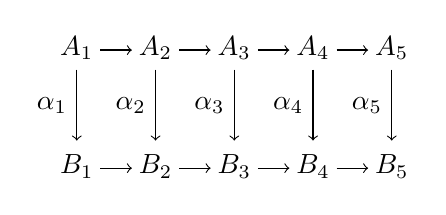
\begin{tikzpicture}
            \node [above] at (0,0) {$B_{1}$};
            \node [above] at (1,0) {$B_{2}$};
            \node [above] at (2,0) {$B_{3}$};
            \node [above] at (3,0) {$B_{4}$};
            \node [above] at (4,0) {$B_{5}$};
            \node [above] at (0,1.5) {$A_{1}$};
            \node [above] at (1,1.5) {$A_{2}$};
            \node [above] at (2,1.5) {$A_{3}$};
            \node [above] at (3,1.5) {$A_{4}$};
            \node [above] at (4,1.5) {$A_{5}$};
            \draw [->] (0.3,0.25) to (0.7,0.25);
            \draw [->] (1.3,0.25) to (1.7,0.25);
            \draw [->] (2.3,0.25) to (2.7,0.25);
            \draw [->] (3.3,0.25) to (3.7,0.25);
            \draw [->] (0.3,1.75) to (0.7,1.75);
            \draw [->] (1.3,1.75) to (1.7,1.75);
            \draw [->] (2.3,1.75) to (2.7,1.75);
            \draw [->] (3.3,1.75) to (3.7,1.75);
            \draw [->] (0,1.5)-- node [left, pos=0.5]{$\alpha_{1}$} (0,0.6);
            \draw [->] (1,1.5)-- node [left, pos=0.5]{$\alpha_{2}$} (1,0.6);
            \draw [->] (2,1.5)-- node [left, pos=0.5]{$\alpha_{3}$} (2,0.6);
            \draw [->] (3,1.5)-- node [left, pos=0.5]{$\alpha_{4}$} (3,0.6);
            \draw [->] (4,1.5)-- node [left, pos=0.5]{$\alpha_{5}$} (4,0.6);
        \end{tikzpicture}
    \end{figure}
    be a commutative diagram of $R$-module homomorphisms, with exact rows. Prove that:
    \begin{enumerate}[(a)]
        \item $\alpha_{1}$ an epimorphism and $\alpha_{2},\alpha_{4}$ monomorphisms $\Rightarrow$ $\alpha_{3}$ is a monomorphism;
        \item $\alpha_{5}$ a monomorphism and $\alpha_{2},\alpha_{4}$ epimorphisms $\Rightarrow$ $\alpha_{3}$ is an epimorphism.
    \end{enumerate}
\end{ex}

\begin{answer}
    Denote all the homomorphisms as following.
    \begin{figure}[H]\centering
        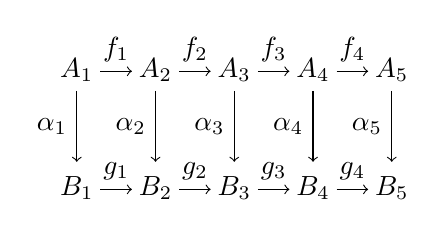
\begin{tikzpicture}
            \node [above] at (0,0) {$B_{1}$};
            \node [above] at (1,0) {$B_{2}$};
            \node [above] at (2,0) {$B_{3}$};
            \node [above] at (3,0) {$B_{4}$};
            \node [above] at (4,0) {$B_{5}$};
            \node [above] at (0,1.5) {$A_{1}$};
            \node [above] at (1,1.5) {$A_{2}$};
            \node [above] at (2,1.5) {$A_{3}$};
            \node [above] at (3,1.5) {$A_{4}$};
            \node [above] at (4,1.5) {$A_{5}$};
            \draw [->] (0.3,0.25)-- node [above, pos=0.5]{$g_{1}$} (0.7,0.25);
            \draw [->] (1.3,0.25)-- node [above, pos=0.5]{$g_{2}$} (1.7,0.25);
            \draw [->] (2.3,0.25)-- node [above, pos=0.5]{$g_{3}$} (2.7,0.25);
            \draw [->] (3.3,0.25)-- node [above, pos=0.5]{$g_{4}$} (3.7,0.25);
            \draw [->] (0.3,1.75)-- node [above, pos=0.5]{$f_{1}$} (0.7,1.75);
            \draw [->] (1.3,1.75)-- node [above, pos=0.5]{$f_{2}$} (1.7,1.75);
            \draw [->] (2.3,1.75)-- node [above, pos=0.5]{$f_{3}$} (2.7,1.75);
            \draw [->] (3.3,1.75)-- node [above, pos=0.5]{$f_{4}$} (3.7,1.75);
            \draw [->] (0,1.5)-- node [left, pos=0.5]{$\alpha_{1}$} (0,0.6);
            \draw [->] (1,1.5)-- node [left, pos=0.5]{$\alpha_{2}$} (1,0.6);
            \draw [->] (2,1.5)-- node [left, pos=0.5]{$\alpha_{3}$} (2,0.6);
            \draw [->] (3,1.5)-- node [left, pos=0.5]{$\alpha_{4}$} (3,0.6);
            \draw [->] (4,1.5)-- node [left, pos=0.5]{$\alpha_{5}$} (4,0.6);
        \end{tikzpicture}
    \end{figure}
    \begin{enumerate}[(a)]
        \item For any $a\in A_{3}$, $\alpha_{3}(a)=0$, we need to show that $a=0$. $g_{3}\alpha_{3}(a)=\alpha_{4}f_{3}(a)=0$, since $\alpha_{4}$ is monomorphism, $f_{3}(a)=0$. So $a\in \mathrm{Ker}f_{3}\Rightarrow a\in \mathrm{Im}f_{2}$. There's $a'\in A_{2}$, $f_{2}(a')=a$, $\alpha_{3}f_{2}(a')=0=g_{2}\alpha_{2}(a')$. So $\alpha_{2}(a')\in \mathrm{Ker}g_{2}=\mathrm{Im}g_{1}$. There is $b''\in B_{1}$, $g_{1}(b'')=\alpha_{2}(a')$. $\alpha_{1}$ is epimorphism so $\exists a''\in A_{1}$, $b''=\alpha_{1}(a'')$, so $g_{1}\alpha_{1}(a'')=\alpha_{2}f_{1}(a'')=\alpha_{2}(a')$. $\alpha_{2}$ is monomorphism so $f_{1}(a'')=a'\in \mathrm{Ker}f_{2}\Rightarrow a=f_{2}(a')=0$.
        \item For any $b\in B_{3}$, we need to show that $b\in \mathrm{Im}\alpha_{3}$. $g_{3}(b)\in B_{4}$, $g_{3}(b)=\alpha_{4}(a')$ for $a'\in A_{4}$ since $\alpha_{4}$ is epimorphism. $g_{4}\alpha_{4}(a')=g_{4}g_{3}(b)=0=\alpha_{5}f_{4}(a')$. $f_{4}a'=0$ cince $\alpha_{5}$ is monomorphism. So there is $a\in A_{3}$, $f_{3}(a)=a'$, $\alpha_{4}f_{3}(a)=g_{3}\alpha_{3}(a)=\alpha_{4}(a')=g_{3}(b)$. $g_{3}(b-\alpha_{3}(a))=0\Rightarrow b-\alpha_{3}(a)\in\mathrm{Ker}g_{3}=\mathrm{Im}g_{2}$. There's $b'\in B_{2}$, $g_{2}(b')=-b+\alpha_{3}(a)$. $\alpha_{2}$ is epimorphism so $\exists a''\in A_{2}$, $\alpha_{2}(a'')=b'$. Consider $\alpha_{3}(a-f_{2}(a''))=\alpha_{3}(a)-\alpha_{3}f_{2}(a'')=-g_{2}\alpha_{2}(a'')+\alpha_{3}(a'')=b$. Thus $b\in \mathrm{Im}\alpha_{3}$, whence $\alpha_{3}$ is epimorphism.
    \end{enumerate}
\end{answer}

$$ $$

\begin{ex}
    \begin{enumerate}[(a)]
        \item If $0\to A\to B\xrightarrow{f} C\to 0$ and $0\to C\xrightarrow{g} D\to D\to E\to 0$ are short exact sequences of modules, then the sequence $0\to A\to B\xrightarrow{gf}D \to E\to 0$ is exact.
        \item Show that every exact sequence may be obtained by splicing together suitable short exact sequences as in (a).
    \end{enumerate}
\end{ex}

\begin{answer}
    \begin{enumerate}[(a)]
        \item The commutative diagram
        \begin{figure}[H]\centering
            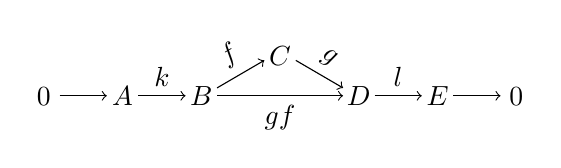
\begin{tikzpicture}
                \node [above] at (0,0) {$0$};
                \node [above] at (1,0) {$A$};
                \node [above] at (2,0) {$B$};
                \node [above] at (4,0) {$D$};
                \node [above] at (5,0) {$E$};
                \node [above] at (6,0) {$0$};
                \node [below] at (3,1) {$C$};
                \draw [->] (0.2,0.25) to (0.8,0.25);
                \draw [->] (1.2,0.25)-- node [above, pos=0.5] {$k$} (1.8,0.25);
                \draw [->] (4.2,0.25)-- node [above, pos=0.5] {$l$} (4.8,0.25);
                \draw [->] (5.2,0.25) to (5.8,0.25);
                \draw [->] (2.2,0.25)-- node [below, pos=0.5] {$gf$} (3.8,0.25);
                \draw [->] (2.2,0.35)-- node [above, pos=0.5, sloped] {$f$} (2.8,0.7);
                \draw [->] (3.2,0.7)-- node [above, pos=0.5, sloped] {$g$} (3.8,0.35);
            \end{tikzpicture}
        \end{figure}
        For any $a\in A$, $k(a)\in \mathrm{Ker}f\Rightarrow fk(a)=0$. $g$ is monomorphism so $\mathrm{Ker}g=0$. Since $gfk(a)=0$, $\mathrm{Im}k\subset \mathrm{Ker}gf$. $\mathrm{Ker}g=0\Rightarrow gf(a)=0$ if and only if $f(a)=0$. $\mathrm{Ker}gf\subset \mathrm{Im}k$. $\mathrm{Im}gf=\mathrm{Im}g$ since $f$ is epimorphism. So $\mathrm{Im}gf=\mathrm{Ker}l$. $0\to A\to B\xrightarrow{gf}D\to E\to 0$ is an exact sequence.
        \item For any finite exact sequence $A_{1}\xrightarrow{f_{1}}A_{2}\xrightarrow{f_{2}}\cdots \xrightarrow{f_{n-1}}A_{n}$. We can add head and tail into it and form
        \[0\to \mathrm{Coker}f_{1}\to A_{1}\xrightarrow{f_{1}}\to A_{2}\xrightarrow{f_{2}}\cdots\xrightarrow{f_{n-1}}A_{n}\to \mathrm{Coim}f_{n-1}\to 0\]
        For any exact sequence which has fragment
        \[A\xrightarrow{f}B\xrightarrow{g}C\xrightarrow{h}D\]
        Consider
        \begin{figure}[H]\centering
            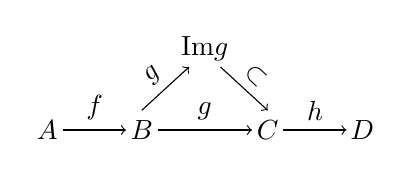
\begin{tikzpicture}
                \node [above] at (0,0) {$A$};
                \node [above] at (1.2,0) {$B$};
                \node [above] at (2.8,0) {$C$};
                \node [above] at (4,0) {$D$};
                \node [above] at (2,1) {$\mathrm{Im}g$};
                \draw [->] (0.2,0.25)-- node [above, pos=0.5] {$f$} (1,0.25);
                \draw [->] (1.4,0.25)-- node [above, pos=0.5] {$g$} (2.6,0.25);
                \draw [->] (3,0.25)-- node [above, pos=0.5] {$h$} (3.8,0.25);
                \draw [->] (1.2,0.5)-- node [above, pos=0.5, sloped] {$g$} (1.8,1.05);
                \draw [->] (2.2,1.05)-- node [above, pos=0.5, sloped] {$\subset$} (2.8,0.5);
            \end{tikzpicture}
        \end{figure}
        $\subset$ is the inclusion map. We can split into $A\xrightarrow{f}B\xrightarrow{g}\mathrm{Im}g\to 0$ and $0\to \mathrm{Im}g\xrightarrow{\subset}C\xrightarrow{h}D$. This provides us a way to split an exact sequence into short exact sequences.
    \end{enumerate}
\end{answer}

$$ $$

\begin{ex}
    Show that isomorphism of short exact sequences is an equivalence relation.
\end{ex}

\begin{answer}
    We check isomorphism of short exact sequence is equivalence relation. $a=0\to A_{1}\to B_{1}\to C_{1}\to 0$, $b=0\to A_{2}\to B_{2}\to C_{2}\to 0$ and $c=0\to A_{3}\to B_{3}\to C_{3}\to 0$.
    \begin{enumerate}
        \item The commutative diagram
        \begin{figure}[H]\centering
            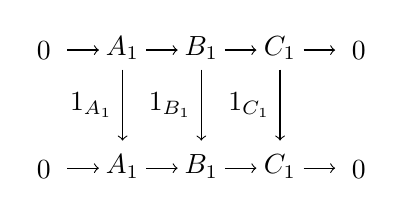
\begin{tikzpicture}
                \node [above] at (0,0) {$0$};
                \node [above] at (1,0) {$A_{1}$};
                \node [above] at (2,0) {$B_{1}$};
                \node [above] at (3,0) {$C_{1}$};
                \node [above] at (4,0) {$0$};
                \node [above] at (0,1.5) {$0$};
                \node [above] at (1,1.5) {$A_{1}$};
                \node [above] at (2,1.5) {$B_{1}$};
                \node [above] at (3,1.5) {$C_{1}$};
                \node [above] at (4,1.5) {$0$};
                \draw [->] (0.3,0.25) to (0.7,0.25);
                \draw [->] (1.3,0.25) to (1.7,0.25);
                \draw [->] (2.3,0.25) to (2.7,0.25);
                \draw [->] (3.3,0.25) to (3.7,0.25);
                \draw [->] (0.3,1.75) to (0.7,1.75);
                \draw [->] (1.3,1.75) to (1.7,1.75);
                \draw [->] (2.3,1.75) to (2.7,1.75);
                \draw [->] (3.3,1.75) to (3.7,1.75);
                \draw [->] (1,1.5)-- node [left, pos=0.5]{$1_{A_{1}}$} (1,0.6);
                \draw [->] (2,1.5)-- node [left, pos=0.5]{$1_{B_{1}}$} (2,0.6);
                \draw [->] (3,1.5)-- node [left, pos=0.5]{$1_{C_{1}}$} (3,0.6);
            \end{tikzpicture}
        \end{figure}
        shows that $a\sim a$ since $1_{A_{1}}$, $1_{B_{1}}$ and $1_{C_{1}}$ are isomorphisms.
        \item If
        \begin{figure}[H]\centering
            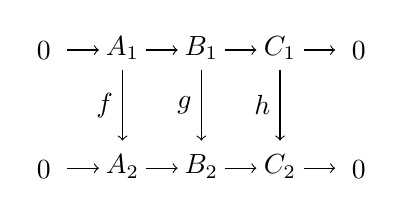
\begin{tikzpicture}
                \node [above] at (0,0) {$0$};
                \node [above] at (1,0) {$A_{2}$};
                \node [above] at (2,0) {$B_{2}$};
                \node [above] at (3,0) {$C_{2}$};
                \node [above] at (4,0) {$0$};
                \node [above] at (0,1.5) {$0$};
                \node [above] at (1,1.5) {$A_{1}$};
                \node [above] at (2,1.5) {$B_{1}$};
                \node [above] at (3,1.5) {$C_{1}$};
                \node [above] at (4,1.5) {$0$};
                \draw [->] (0.3,0.25) to (0.7,0.25);
                \draw [->] (1.3,0.25) to (1.7,0.25);
                \draw [->] (2.3,0.25) to (2.7,0.25);
                \draw [->] (3.3,0.25) to (3.7,0.25);
                \draw [->] (0.3,1.75) to (0.7,1.75);
                \draw [->] (1.3,1.75) to (1.7,1.75);
                \draw [->] (2.3,1.75) to (2.7,1.75);
                \draw [->] (3.3,1.75) to (3.7,1.75);
                \draw [->] (1,1.5)-- node [left, pos=0.5]{$f$} (1,0.6);
                \draw [->] (2,1.5)-- node [left, pos=0.5]{$g$} (2,0.6);
                \draw [->] (3,1.5)-- node [left, pos=0.5]{$h$} (3,0.6);
            \end{tikzpicture}
        \end{figure}
        then we have
        \begin{figure}[H]\centering
            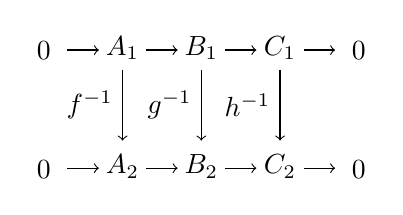
\begin{tikzpicture}
                \node [above] at (0,0) {$0$};
                \node [above] at (1,0) {$A_{2}$};
                \node [above] at (2,0) {$B_{2}$};
                \node [above] at (3,0) {$C_{2}$};
                \node [above] at (4,0) {$0$};
                \node [above] at (0,1.5) {$0$};
                \node [above] at (1,1.5) {$A_{1}$};
                \node [above] at (2,1.5) {$B_{1}$};
                \node [above] at (3,1.5) {$C_{1}$};
                \node [above] at (4,1.5) {$0$};
                \draw [->] (0.3,0.25) to (0.7,0.25);
                \draw [->] (1.3,0.25) to (1.7,0.25);
                \draw [->] (2.3,0.25) to (2.7,0.25);
                \draw [->] (3.3,0.25) to (3.7,0.25);
                \draw [->] (0.3,1.75) to (0.7,1.75);
                \draw [->] (1.3,1.75) to (1.7,1.75);
                \draw [->] (2.3,1.75) to (2.7,1.75);
                \draw [->] (3.3,1.75) to (3.7,1.75);
                \draw [->] (1,1.5)-- node [left, pos=0.5]{$f^{-1}$} (1,0.6);
                \draw [->] (2,1.5)-- node [left, pos=0.5]{$g^{-1}$} (2,0.6);
                \draw [->] (3,1.5)-- node [left, pos=0.5]{$h^{-1}$} (3,0.6);
            \end{tikzpicture}
        \end{figure}
        is also commutative. So $a\sim b\Leftrightarrow b\sim a$.
        \item If
        \begin{figure}[H]\centering
            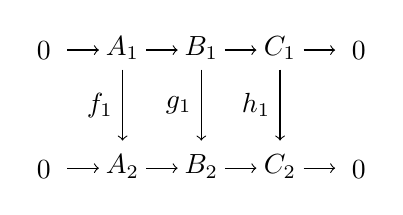
\begin{tikzpicture}
                \node [above] at (0,0) {$0$};
                \node [above] at (1,0) {$A_{2}$};
                \node [above] at (2,0) {$B_{2}$};
                \node [above] at (3,0) {$C_{2}$};
                \node [above] at (4,0) {$0$};
                \node [above] at (0,1.5) {$0$};
                \node [above] at (1,1.5) {$A_{1}$};
                \node [above] at (2,1.5) {$B_{1}$};
                \node [above] at (3,1.5) {$C_{1}$};
                \node [above] at (4,1.5) {$0$};
                \draw [->] (0.3,0.25) to (0.7,0.25);
                \draw [->] (1.3,0.25) to (1.7,0.25);
                \draw [->] (2.3,0.25) to (2.7,0.25);
                \draw [->] (3.3,0.25) to (3.7,0.25);
                \draw [->] (0.3,1.75) to (0.7,1.75);
                \draw [->] (1.3,1.75) to (1.7,1.75);
                \draw [->] (2.3,1.75) to (2.7,1.75);
                \draw [->] (3.3,1.75) to (3.7,1.75);
                \draw [->] (1,1.5)-- node [left, pos=0.5]{$f_{1}$} (1,0.6);
                \draw [->] (2,1.5)-- node [left, pos=0.5]{$g_{1}$} (2,0.6);
                \draw [->] (3,1.5)-- node [left, pos=0.5]{$h_{1}$} (3,0.6);
            \end{tikzpicture}
        \end{figure}
        and
        \begin{figure}[H]\centering
            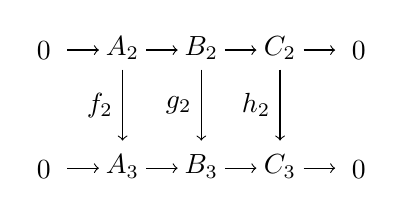
\begin{tikzpicture}
                \node [above] at (0,0) {$0$};
                \node [above] at (1,0) {$A_{3}$};
                \node [above] at (2,0) {$B_{3}$};
                \node [above] at (3,0) {$C_{3}$};
                \node [above] at (4,0) {$0$};
                \node [above] at (0,1.5) {$0$};
                \node [above] at (1,1.5) {$A_{2}$};
                \node [above] at (2,1.5) {$B_{2}$};
                \node [above] at (3,1.5) {$C_{2}$};
                \node [above] at (4,1.5) {$0$};
                \draw [->] (0.3,0.25) to (0.7,0.25);
                \draw [->] (1.3,0.25) to (1.7,0.25);
                \draw [->] (2.3,0.25) to (2.7,0.25);
                \draw [->] (3.3,0.25) to (3.7,0.25);
                \draw [->] (0.3,1.75) to (0.7,1.75);
                \draw [->] (1.3,1.75) to (1.7,1.75);
                \draw [->] (2.3,1.75) to (2.7,1.75);
                \draw [->] (3.3,1.75) to (3.7,1.75);
                \draw [->] (1,1.5)-- node [left, pos=0.5]{$f_{2}$} (1,0.6);
                \draw [->] (2,1.5)-- node [left, pos=0.5]{$g_{2}$} (2,0.6);
                \draw [->] (3,1.5)-- node [left, pos=0.5]{$h_{2}$} (3,0.6);
            \end{tikzpicture}
        \end{figure}
        are commutative. Then
        \begin{figure}[H]\centering
            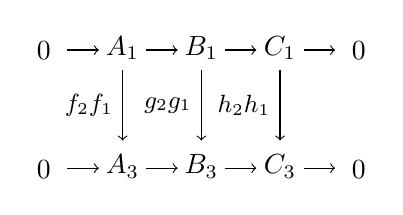
\begin{tikzpicture}
                \node [above] at (0,0) {$0$};
                \node [above] at (1,0) {$A_{3}$};
                \node [above] at (2,0) {$B_{3}$};
                \node [above] at (3,0) {$C_{3}$};
                \node [above] at (4,0) {$0$};
                \node [above] at (0,1.5) {$0$};
                \node [above] at (1,1.5) {$A_{1}$};
                \node [above] at (2,1.5) {$B_{1}$};
                \node [above] at (3,1.5) {$C_{1}$};
                \node [above] at (4,1.5) {$0$};
                \draw [->] (0.3,0.25) to (0.7,0.25);
                \draw [->] (1.3,0.25) to (1.7,0.25);
                \draw [->] (2.3,0.25) to (2.7,0.25);
                \draw [->] (3.3,0.25) to (3.7,0.25);
                \draw [->] (0.3,1.75) to (0.7,1.75);
                \draw [->] (1.3,1.75) to (1.7,1.75);
                \draw [->] (2.3,1.75) to (2.7,1.75);
                \draw [->] (3.3,1.75) to (3.7,1.75);
                \draw [->] (1,1.5)-- node [left, pos=0.5]{\small{$f_{2}f_{1}$}} (1,0.6);
                \draw [->] (2,1.5)-- node [left, pos=0.5]{\small{$g_{2}g_{1}$}} (2,0.6);
                \draw [->] (3,1.5)-- node [left, pos=0.5]{\small{$h_{2}h_{1}$}} (3,0.6);
            \end{tikzpicture}
        \end{figure}
        is also commutative. So $a\sim b, b\sim c\Rightarrow a\sim c$.
    \end{enumerate}
\end{answer}

$$ $$

\begin{ex}
    If $f:A\to B$ and $g:B\to A$ are $R$-module homomorphisms such that $gf=1_{A}$, then $B=\mathrm{Im}f\oplus \mathrm{Ker}g$.
\end{ex}

\begin{answer}
    $gf=1_{A}$ so $f$ is monomorphism and $g$ is epimorphism. So $B /\mathrm{Ker}g\cong \mathrm{Im}g=A\cong A /{0}\cong \mathrm{Im}f$. $\mathrm{Ker}g\cap \mathrm{Im}0=\{0\}$ since $g(\mathrm{Im}f)=A$. Thus $B=\mathrm{Ker}g\oplus\mathrm{Im}f$.
\end{answer}

$$ $$

\begin{ex}
    Let $R$ be a ring and $R^{op}$ its opposite ring. If $A$ is a left $R$-module, then $A$ is a right $R^{op}$-module such that $ra=ar$ for all $a\in A, 4\in R, r\in R^{op}$.
\end{ex}

\begin{answer}
    Trivial.
\end{answer}

$$ $$

\begin{ex}
    \begin{enumerate}[(a)]
        \item If $R$ has an identity and $A$ is an $R$-module, then there are submodules $B$ and $C$ of $A$ such that $B$ is unitary, $RC=0$ and $A=B\oplus C$.
        \item Let $A_{1}$ be another $R$-module, with $A_{1}=B_{1}\oplus C_{1}$ ($B_{1}$ unitary, $RC=0$), If $f:A\to A_{1}$ is an $R$-module homomorphism then $f(B)\subset B_{1}$ and $f(C)\subset C_{1}$.
        \item If the map $f$ of part (b) is an epimorphism, then so are $f|B:B\to B_{1}$ and $f|C:C\to C_{1}$.
    \end{enumerate}
\end{ex}

\begin{answer}
    \begin{enumerate}[(a)]
        \item Let $B=\{1_{R}a|a\in A\}$, $C=\{a\in A|1_{R}a=0\}$. Then $B$ is unitary since $1_{R}(1_{R}a)=1_{R}a$. $RC=0$ since $ra=(r1_{R})a=r(1_{R}a)=0 \forall a\in C$. And $\forall a\in A$, $1_{R}(a-1_{R}a)=0\Rightarrow a-1_{R}a\in C$. So $A=\subset B\oplus C$. Obviously $B\oplus C\subset A$, $A=B\oplus C$.
        \item For any $x=b_{1}+c_{1}\in A_{1}$, $1_{R}x=1_{R}(b_{1}+c_{1})=1_{R}b_{1}$, $B_{1}$ is the maximal unitary submodule and $B_{1}$ contains all unitary elements. $f(B)$ is also unitary since $f(b)=f(1_{R}b)=1_{R}f(b)$ for any $b\in B$. $f(B)\subset B_{1}$.
        
        $C_{1}$ contains all elements $x\in A_{1}$ s.t. $Rx=0$. Since $Rf(c)=f(Rc)=0$ for all $c\in C$, we have $f(C)\subset C_{1}$.
        \item For any $b'\in B'$, we have $f(x)=b'$ since $f$ is epimorphism. Assume $x=b+c$ with $b\in B$ and $c\in C$. $f(x)=f(1_{R}(b+c))=f(1_{R}b)=1_{R}f(b)=f(b)$. So $\exists b\in B$, $f(b)=b'$. $f|B$ is epimorphism. For any $c'\in C$, we have $f(y)=c$. Assume $y=a+d$ with $a\in B$ and $d\in C$. $f(y)=f(1_{R}(a+d))=f(1_{R}a)=0$, so $1_{R}f(a)=0\Rightarrow a=0$. Thus $\exists y=d\in C$, $f(d)=c'$. $f|C$ is epimorphism.
    \end{enumerate}
\end{answer}

$$ $$

\begin{ex}
    Let $R$ be a ring without identity. Embed $R$ in a ring $S$ with identity and charateristic zero as in the proof of Theorem III.1.10. Identify $R$ with its image in $S$.
    \begin{enumerate}[(a)]
        \item Show that every element of $S$ may be uniquely expressed in the form $r1_{S}+n1_{S}(r\in R, n\in \mathbf{Z})$.
        \item If $A$ is an $R$-module and $a\in A$, show that there is a unique $R$-module homomorphism $f:S\to A$ such that $f(1_{S})=a$.
    \end{enumerate}
\end{ex}

\begin{answer}
    \begin{enumerate}[(a)]
        \item Trivial since $S=R\times \mathbf{Z}$.
        \item $S=R1_{S}\oplus\mathbf{Z}1_{S}$. Let $f(r1_{S}+n1_{S})=ra+na$, then $f(1_{S})=a$ and $f$ is a well defined homomorphism of modules. If there exists another $g$ s.t. $g(1_{S})=a$, $\forall r1_{S}+n1_{S}\in S$, $g(r1_{S}+n1_{S})=rg(1_{S})+ng(1_{S})=ra+na=f(r1_{S}+n1_{S})$. So $g=f$.
    \end{enumerate}
\end{answer}
\end{document}